\documentclass{article}
\usepackage{pgffor, siunitx}
\usepackage{import}
\usepackage{graphicx} % Allows image inclusion
\usepackage{wrapfig}
\usepackage{float}
\usepackage{svg}
\usepackage[hidelinks]{hyperref}
\usepackage{tikz}
\usetikzlibrary{arrows.meta}
\usetikzlibrary{calc}
\usetikzlibrary{matrix}

% Matematik
\usepackage{amssymb}  % most common
\usepackage{amsmath, mathrsfs, pgfmath}

\usepackage{ifthen}

% Værktøjer
% Til at folde lister ud med 
\newcounter{vaerdiet}
\newcounter{vaerdito}                           % Numerisk 
\newcounter{vaerditre}
\newcounter{vaerdifire}
\newcommand{\vaerdifem}{-\infty}
\newcommand{\vaerdiseks}{\infty}                % Symbolsk
\newcommand{\vaerdisyv}{-\infty}
\newcommand{\vaerdiotte}{\infty}                

\def\register#1#2{\registerAllokering#2\nil{#1}}
\def\registerAllokering#1,#2\nil#3{
    \ifcase#3                                   % Register 1 ( Numerisk)
        \setcounter{vaerdiet}{#2}
        \setcounter{vaerdito}{#1}
    \or                                         % Register 2 ( Numerisk)
        \setcounter{vaerditre}{#2}
        \setcounter{vaerdifire}{#1}
    \or                                         % Register 3 ( Symbols)
        \edef\vaerdifem{#2}                
        \edef\vaerdiseks{#1}
    \or 
        \edef\vaerdisyv{#2}                
        \edef\vaerdiotte{#1}
    \else
        %   
    \fi
}
\def\registeret#1,#2\nil{%
    \setcounter{vaerdiet}{#1}
    \setcounter{vaerdito}{#2}
}%
\def\registerto#1,#2\nil{%
    \setcounter{vaerditre}{#1}
    \setcounter{vaerdifire}{#2}
}%
\def\registertre#1,#2\nil{%                     % Symbolsk register
    \edef\vaerdifem{#1}                
    \edef\vaerdiseks{#2}
}%
\def\registerfire#1,#2\nil{%                     % Symbolsk register
    \edef\vaerdisyv{#1}                
    \edef\vaerdiotte{#2}
}%
\newcommand{\udfold}[2]{
    \ifnum#1=1
        % \registeret#2\nil
        \registerto#2\nil           % Numerisk
    \else
        \ifnum#1=0
            \registeret#2\nil       % Numerisk
        \else   
            \ifnum#1=2
                \registertre#2\nil  % Symbolsk 
            \else
                \registerfire#2\nil % Symbolsk 
            \fi
        \fi
    \fi
}

% Tekst redigering 
\newcommand{\tab}[1]{
    \foreach \i in {0, ..., #1} {
        \quad
    }}
\newcommand{\transformation}[1]{\tab{0}\overset{\mathscr{#1}}{\leftrightarrow}\tab{0}}

% Counters 
\newcounter{kapitel}
\newcounter{alfabetTabular}
\newcounter{eksamensOpgave}
\renewcommand{\thealfabetTabular}{\alph{alfabetTabular}}

% Kapitel Context 
\newenvironment{kapitel}[1][]{
    \clearpage
    \refstepcounter{kapitel} % Increment counter first
    \subsection*{Kapitel \thekapitel: #1}
}{}

% Formelsamling / Opgaver / Øvelser mm...
\newenvironment{rubrik}[1][]{
    \clearpage
    \section*{#1}
    \addcontentsline{toc}{section}{#1}
    \setcounter{kapitel}{0} % Nulstil counteren, I tilfælde af, at den har været brugt. 
}{}

\newenvironment{underrubrik}[1][]{
    \subsection*{#1}
    \addcontentsline{toc}{subsection}{#1}
}{}

% Eksamensopgave context 
\newenvironment{eksamensOpgave}[1][]{
    \refstepcounter{eksamensOpgave} % Increment counter first
    \subsection*{Opgave \theeksamensOpgave: #1}
    \setcounter{alfabetTabular}{0}
}{}



% Indhold
\newenvironment{Formelsamling}{\begin{rubrik}[Formelsamling]\end{rubrik}}{}
\newenvironment{Udledninger}{\begin{rubrik}[Udledninger]\end{rubrik}}{}

\newenvironment{Opgaver}{\begin{rubrik}[Opgaver]\end{rubrik}}{}
\newenvironment{Opgave}[1][]{\begin{underrubrik}[#1]\end{underrubrik}\setcounter{alfabetTabular}{0}}{\vspace{100pt}}
\newenvironment{UnderOpgave}[1][]{
    \refstepcounter{alfabetTabular}
    \subsubsection*{\boldmath{\thealfabetTabular. #1}}}{}

\newenvironment{Øvelser}{\begin{rubrik}[Øvelser]\end{rubrik}}{}
\newenvironment{Øvelse}[1][]{\begin{underrubrik}[#1]\end{underrubrik}}{}

\newenvironment{Udklip}{\color{red}\begin{underrubrik}\end{underrubrik}}{}              % Skal bruges til når jeg retter opgaver, så fletter jeg de forkerte ind i det her. 


%  _____  _____  ___________   ____  ______  ___              _______     __________
%    |      |               |   | \ /         |              |       \   |          
%    |      |               |   |  \          |              |        |  |          
%    |------|               |   |---\------   |              |_______/   |------    
%    |      |    ____       |   |    \        |       ___    |           |          
%  __|__  __|__    \_______/   _|_   _\____    \_______/   __|__         |__________

%   __________  ___      ___   _____    _____  _____   ____  ____________  ____________    _______     _____    _____   __________     _______     
%  |             |        |    |  \      |      |    __/          |             |        /       \     |  \      |    |              |        \   
%  |             |        |    |   \     |      | __/             |             |       |         |    |   \     |    |              |        |   
%  |------       |        |    |    \    |      |/\__             |             |       |         |    |    \    |    |------        |________/   
%  |             |        |    |     \   |      |   \__           |             |       |         |    |     \   |    |              |        \   
%  |              \______/   __|__    \__|    __|__  __\__       _|_      ______|_____   \_______/   __|__    \__|    |__________  __|__       \__




% ------- Fortegn -------
% Indstillinger:
% Vaerdiet = 0  ->  + ax 
% Vaerdiet = 1  ->  ax
% 
% Parametre: 
% {a}{x} 
%     
% Logik: 
% 1x            ->  x. 
% -1x           ->  -x
% 0x            ->  ""
\newcommand{\fortegn}[2]{                       % {a}{x}
    \pgfmathparse{abs(#1 - int(#1)) > 0}             % 1.5 - 1 > 0 ? 
    % \pgfmathparse{#1 - int(#1) < 0}             % -1.5 - (-1) < 0 ? 
    \ifnum\pgfmathresult=1                      % Integer vs float check
    % Decimaltal
        \pgfmathparse{ifthenelse(#1<0, "", ifthenelse(\thevaerdiet==1, "", "+"))} % a < 0 ?    Første tal ? 
        \pgfmathresult #1#2 
    \else
    % Heltal
        \ifnum#1=0                              % a = 0 
        % Kommentar så kompiler virker.
        \else
            \ifnum#1=1
                \ifnum\thevaerdiet=1
                    #2                          % x
                \else 
                    + #2                        % +x
                \fi
            \else
                \ifnum#1=-1
                    - #2                        % -x
                \else
                    \ifnum#1>0
                        \ifnum\thevaerdiet=1
                            #1#2                % +ax
                        \else 
                            + #1#2              % ax
                        \fi
                    \else
                        #1#2                    % -ax
                    \fi
                \fi
            \fi
        \fi
    \fi
}
%\symbolEllerEj{2}  <- Ikke et symbol
%\symbolEllerEj{a}  <- Symbol
% Skal have formen \ifcsname #1\endcsname ikke \ifcsname #1 \endcsname
\newcommand{\erSymbol}[3]{ \ifcsname #1\endcsname                                           #2 \else #3 \fi }
                                            % |a - int(a)| > 0 ? 
\newcommand{\erDecimal}[3] { \pgfmathparse{abs(#1 - int(#1)) > 0} \ifnum\pgfmathresult=1    #2 \else #3 \fi }
  


\newcommand{\fortegnTo}[2]{                       % {a}{x}
    \erSymbol{#1}{
        % Er symbol
        - #1#2
    }{
        \erDecimal{#1}{
            % Er decimal
            \pgfmathparse{ifthenelse(#1<0, "", ifthenelse(\thevaerdiet==1, "", "+"))} % a < 0 ?    Første tal ? 
            \pgfmathresult #1#2 
        }{
            % Er heltal
            \ifnum#1=0                              % a = 0 
            % Kommentar så kompiler virker.
            \else
                \ifnum#1=1
                    \ifnum\thevaerdiet=1
                        #2                          % x
                    \else 
                        + #2                        % +x
                    \fi
                \else
                    \ifnum#1=-1
                        - #2                        % -x
                    \else
                        \ifnum#1>0
                            \ifnum\thevaerdiet=1
                                #1#2                % +ax
                            \else 
                                + #1#2              % ax
                            \fi
                        \else
                            #1#2                    % -ax
                        \fi
                    \fi
                \fi
            \fi
        }
    }
}









% ------- differensLigning -------

% Indstillinger:
% 
% Parametre: 
% {a}{b}{y}{x} 
%     
% Logik: 
% y[n] = sum(ay[n - i]) + b0x[n] + sum(bx[n - i])
\newcommand{\differensLigning}[4]{ 
    \register{0}{0, 1}                              % Startværdier sættes til 0. 
    y[n] = 
    \foreach \a [count=\i from 1] in {#1} {
        \fortegn{\a}{#3[n - \i]}
        \ifnum\thevaerdiet=1\register{0}{0, 0}\fi   % Første værdi sat 
    }
    \foreach \b [count=\i from 0] in {#2} {
        \ifnum\i=0
            \fortegn{\b}{#4[n]}
        \else   
            \fortegn{\b}{#4[n - \i]}
        \fi
        \ifnum\thevaerdiet=1\register{0}{0, 0}\fi   % Første værdi sat 
    }
}

% -------- filterZ --------

% Indstillinger:
% 
% Parametre: 
% {b_0, ..., b_N}{a_0, ..., a_N}
%     
% Logik: 
% (1 + 2z^-1)/(1 + 2z^-1 + 3z^-2)

% Hvad jeg ønsker. Fortegn virker dog ikke med decimaler.
\newcommand{\filterZto}[2]{
    \frac{
        \register{2}{0, 1}                                  % Første værdi mangler
        \foreach \b [count=\i from 0] in {#1} {
            \ifnum\i=0 \b \else \fortegnTo{\b}{z^{-\i}}\fi    % b eller bz^-i ? 
            \ifnum\vaerdifem=1\register{2}{0, 0}\fi
            % \ifnum\vaerdifem=1\register{2}{0, 0}\fi       % Værdi er sat
        }
    }{
        \register{2}{0, 1}                                  % Første værdi mangler
        \foreach \a [count=\i from 0] in {#2} {
            \ifnum\i=0 \a \else \fortegnTo{\a}{z^{-\i}}\fi    % a eller az^-i ? 
            \ifnum\vaerdiseks=1\register{2}{0, 0}\fi       % Værdi er sat
        }
    }
}
\newcommand{\filterZ}[2]{
    \frac{\foreach \b [count=\i from 0] in {#1}{
        \ifnum\i=0
            \b
        \else
            \pgfmathparse{ifthenelse(\b<0, "", "+")}\pgfmathresult \b z^{-\i}
        \fi}
    }{\foreach \a [count=\i from 0] in {#2}{
        \ifnum\i=0
            \a
        \else
            \pgfmathparse{ifthenelse(\a<0, "", "+")}\pgfmathresult \a z^{-\i}
        \fi}
    }
}





\newcommand{\convolutionNum}[3] { % View, Grænser, indhold. 
    \udfold{0}{#2}                                  % Udfolder grænser til registre. 
    y[n]   
    \ifnum#1=1                                      % View 1
        = x[n]\star h[n]
    \else 
        \ifnum#1=0                                  % View 2
            = \sum_{n = \thevaerdiet}^{\thevaerdito}{#3}
        \else                                       % View 3
            = x[n]\star h[n] = \sum_{n = \thevaerdiet}^{\thevaerdito}{#3}
        \fi
    \fi
}
\newcommand{\convolutionSym}[3] { % View, Grænser, (x, h) 
    \udfold{2}{#2}                                  % Udfolder grænser til registre. 
    \udfold{3}{#3}                                  % Udfolder grænser til registre.
    \ifnum#1=1                                      % View 1
        \vaerdisyv[k]\star \vaerdiotte[k]
    \else 
        \ifnum#1=0                                  % View 2
            \sum_{k = \vaerdifem}^{\vaerdiseks}{\vaerdisyv[k] * \vaerdiotte[n-k]}
        \else                                       % View 3
            \vaerdisyv[k]\star \vaerdiotte[k] = \sum_{k = \vaerdifem}^{\vaerdiseks}{\vaerdisyv[k] * \vaerdiotte[n-k]}
        \fi
    \fi
}
\newcommand{\convolution}[2]{
    y[n] = #1[n]\star #2[n] = \sum_{k = -\infty}^{\infty}{#1[k]* #2[n-k]}   
}

\newcommand{\infsum}[2]{\sum_{#1 = -\infty}^{\infty}{#2}}


\newcommand{\cosTilEksponentiel}[1]{ \frac{e^{j#1} + e^{-j#1}}{2} }
\newcommand{\sinTilEksponentiel}[1]{ \frac{e^{j#1} - e^{-j#1}}{2j} }


\newcommand{\lavKolonneData}[3]{  
    % Store in the column variables (c1, c2, c3,...)
    \expandafter\xdef\csname c1\the\numexpr\value{raekketaeller}+1\endcsname{#1}  
    \expandafter\xdef\csname c2\the\numexpr\value{raekketaeller}+1\endcsname{#2}  
    \expandafter\xdef\csname c3\the\numexpr\value{raekketaeller}+1\endcsname{#3}  
    
    % Increment the column counter for the next column
    \stepcounter{raekketaeller}  
}
% Set up a counter to keep track of the column number
\newcounter{raekketaeller}\setcounter{raekketaeller}{0}


\NewDocumentEnvironment{EgenTabel}{+b}{
    % ------- Lav dataen -------
    #1 
}{
    % ------- Vis dataen -------
    \vspace{10pt}
    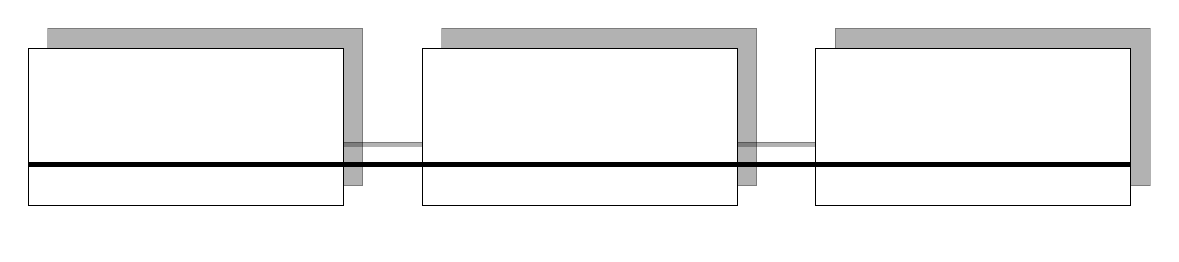
\begin{tikzpicture}
        \tikzset{
            shadow/.style={fill=black, opacity=0.3},        % Skygge 
            cell/.style={fill=white, draw=black, very thin}, % Celle 
        }
        % Baggrund of celler
        \filldraw[shadow] (0.25, 0.5*\theraekketaeller + 2 + 0.25 - 1.5) rectangle(12, 0.5*\theraekketaeller + 2 + 0.25 - 1.5 + 0.05);
        \foreach \x in {0, ..., 2} {
            \filldraw[shadow] (\x*5 + 0.25, 0.25) rectangle(\x*5 + 4.25, 0.5*\theraekketaeller + 2 + 0.25); 
            \filldraw[cell] (\x*5, 0) rectangle(\x*5 + 4, 0.5*\theraekketaeller + 2); 
        }
        % Visning af data.
        \foreach \i in {1, 2, ..., \theraekketaeller} {
            \ifnum\i=1
                \filldraw[black] (0.5, 0.5*\theraekketaeller + 2 - 0.75) node[anchor=west] {$\csname c1\i\endcsname$};
                \filldraw[black] (5.5, 0.5*\theraekketaeller + 2 - 0.75) node[anchor=west] {$\csname c2\i\endcsname$};                
                \filldraw[black] (10.5,0.5*\theraekketaeller + 2 - 0.75) node[anchor=west] {$\csname c3\i\endcsname$};
            \else
                \filldraw[black] (0.5, 0.5*\theraekketaeller + 2 - 1.25 - 0.5*\i) node[anchor=west]{$\csname c1\i\endcsname$};
                \filldraw[black] (5.5, 0.5*\theraekketaeller + 2 - 1.25 - 0.5*\i) node[anchor=west]{$\csname c2\i\endcsname$};
                \filldraw[black] (10.5, 0.5*\theraekketaeller + 2 - 1.25 - 0.5*\i) node[anchor=west]{$\csname c3\i\endcsname$};
            \fi
        }
        % Horinsontal linje. 
        \filldraw[black] (0, 0.5*\theraekketaeller + 2 - 1.5) rectangle(14, 0.5*\theraekketaeller + 2 - 1.5 + 0.05);
    \end{tikzpicture}\setcounter{raekketaeller}{0}
}








% Indhold
\graphicspath{{Indhold/Billeder/}}
% Indstillinger: 
% Billednr:69

\newcommand{\fetchBillede}[2]{\includegraphics[scale=#2]{#1}}
\newcommand{\fetchSVG}[2]{\includesvg[scale=#2]{#1}} % width=1.0\textwidth
\newcommand{\fig}[2]{
    \begin{figure}[h!]
        % \centering
        % \top
        \makebox[\textwidth]{
            \fetchBillede{#1}{#2}
        }
        \caption{#1}
        \label{fig:#1}
    \end{figure}
}



\newcommand{\figSVG}[2]{
    \begin{figure}[h!]
        \centering
        \makebox[\textwidth]{
            \fetchSVG{#1}{#2}
        }
        \caption{#1}
        \label{fig:#1}
    \end{figure}
}


% \figen{0.2} => scaling = 0.2
\newcommand{\figen}[1]{\fig{Z transformations egenskaber}{#1}}
\newcommand{\figto}[1]{\fig{Blokdiagram kapitel 2.png}{#1}}
\newcommand{\figtre}[1]{\figSVG{Feedback system.svg}{#1}}
\newcommand{\figfire}[1]{\fig{Opgave 2.1.png}{#1}}
\newcommand{\figfem}[1]{\fig{Opgave 2.3.png}{#1}}
\newcommand{\figseks}[1]{\fig{Opgave 2.5.png}{#1}}
\newcommand{\figsyv}[1]{\fig{Opgave til kapitel 2.png}{#1}}
\newcommand{\figotte}[1]{\fig{Opgave 2.17.a.png}{#1}}
\newcommand{\figni}[1]{\fig{Opgave 2.17.b.png}{#1}}
\newcommand{\figti}[1]{\fig{Opgave 2.17.c.png}{#1}}
\newcommand{\figeleve}[1]{\fig{Opgave 2.17.png}{#1}}
\newcommand{\figtolv}[1]{\fig{Opgave 2.33.png}{#1}}
\newcommand{\figtretten}[1]{\figSVG{Opgave 2.50.svg}{#1}}
\newcommand{\figfjorten}[1]{\fig{Opgave 2.50.png}{#1}}
\newcommand{\figfemten}[1]{\fig{Opgave 3.1.a.png}{#1}}
\newcommand{\figseksten}[1]{\fig{Opgave 3.1.b.png}{#1}}
\newcommand{\figsytten}[1]{\fig{Opgave 3.1.d.png}{#1}}
\newcommand{\figatten}[1]{\fig{SløretBillede.png}{#1}}
\newcommand{\fignitten}[1]{\fig{AfsløretBillede.png}{#1}}
\newcommand{\figtyve}[1]{\fig{AfsløretsFilter.png}{#1}}
\newcommand{\figenogtyve}[1]{\fig{Opgave 3.15.png}{#1}}
\newcommand{\figtoogtyve}[1]{\fig{Opgave 3.16.png}{#1}}
\newcommand{\figtreogtyve}[1]{\fig{Opgave 3.19 - pzmap.png}{#1}}
\newcommand{\figfireogtyve}[1]{\fig{Opgave 3.19 - Respons.png}{#1}}
\newcommand{\figfemogtyve}[1]{\fig{Opgave 5.2.png}{#1}}
\newcommand{\figseksogtyve}[1]{\fig{Opgave 5.2.e.png}{#1}}
\newcommand{\figsyvogtyve}[1]{\fig{Opgave 5.30.png}{#1}}
\newcommand{\figotteogtyve}[1]{\fig{Opgave 5.48.png}{#1}}
\newcommand{\figniogtyve}[1]{\fig{Opgave 5.48.2.png}{#1}}
\newcommand{\figtredive}[1]{\fig{EKGdata.png}{#1}}
\newcommand{\figenogtredive}[1]{\fig{EKGfrekvenspektrum.png}{#1}}
\newcommand{\figtoogtredive}[1]{\fig{EKGnotchfilterAnalyse.png}{#1}}
\newcommand{\figtreogtredive}[1]{\fig{EKGnotchfilterPZmap.png}{#1}}
\newcommand{\figfireogtredive}[1]{\fig{EKGsignalfiltreret.png}{#1}}
\newcommand{\figfemogtredive}[1]{\fig{EKGforbedretNotchfilterAnalyse.png}{#1}}
\newcommand{\figseksogtredive}[1]{\fig{EKGforbedretNotchfilterPZmap.png}{#1}}
\newcommand{\figsyvogtredive}[1]{\fig{EKGforbedretSignalFiltrering.png}{#1}}
\newcommand{\figotteogtredive}[1]{\fig{SignalbehandlingTemperaturdata.png}{#1}}
\newcommand{\figniogtredive}[1]{\fig{SignalbehandlingTemperaturdataFiltreret.png}{#1}}
\newcommand{\figfyrre}[1]{\fig{SignalbehandlingTemperaturdataFilteranalyse.png}{#1}}
\newcommand{\figenogfyrre}[1]{\fig{SignalbehandlingTemperaturdataIIRFiltermodFIRFilter.png}{#1}}
\newcommand{\figtoogfyrre}[1]{\fig{Signalbehandling3DAudioelev50H50e096a.png}{#1}}
\newcommand{\figtreogfyrre}[1]{\fig{FilterStabilitet.png}{#1}}
\newcommand{\figfireogfyrre}[1]{\fig{Opgave 5.16.png}{#1}}
\newcommand{\figfemogfyrre}[1]{\fig{Opgave 5.31b.png}{#1}}
\newcommand{\figseksogfyrre}[1]{\fig{Opgave 5.31c.png}{#1}}
\newcommand{\figsyvogfyrre}[1]{\fig{Opgave 5.38.b.png}{#1}}
\newcommand{\figotteogfyrre}[1]{\fig{Opgave 5.38.c.png}{#1}}
\newcommand{\figniogfyrre}[1]{\fig{Opgave 5.55.a.png}{#1}}
\newcommand{\fighalvtreds}[1]{\fig{Opgave 5.55.b.png}{#1}}
\newcommand{\figenoghalvtreds}[1]{\fig{Opgave 5.55.c.png}{#1}}
\newcommand{\figtooghalvtreds}[1]{\fig{Opgave 5.55.d.png}{#1}}
\newcommand{\figtreoghalvtreds}[1]{\fig{Opgave 5.39.a.png}{#1}}
\newcommand{\figfireoghalvtreds}[1]{\fig{Opgave 5.39.b.png}{#1}}
\newcommand{\figfemoghalvtreds}[1]{\fig{Opgave 5.39.c.png}{#1}}
\newcommand{\figseksoghalvtreds}[1]{\fig{Opgave 5.39.d.png}{#1}}
\newcommand{\figsyvoghalvtreds}[1]{\fig{Opgave 6.2.a.png}{#1}}
\newcommand{\figotteoghalvtreds}[1]{\fig{Opgave 6.2.b.png}{#1}}
\newcommand{\fignioghalvtreds}[1]{\fig{Opgave 6.2.c.png}{#1}}
\newcommand{\figtres}[1]{\fig{Opgave 6.12.png}{#1}}
\newcommand{\figenogtres}[1]{\fig{Opgave 6.12.Rekonstruering.png}{#1}}
\newcommand{\figtoogtres}[1]{\fig{Opgave 7.1.png}{#1}}
\newcommand{\figtreogtres}[1]{\fig{Opgave 7.1.c.png}{#1}}
\newcommand{\figfireogtres}[1]{\fig{Opgave 7.3.b.png}{#1}}
\newcommand{\figfemogtres}[1]{\fig{Opgave 7.3.c.png}{#1}}
\newcommand{\figseksogtres}[1]{\fig{Opgave 7.3.d.png}{#1}}
\newcommand{\figsyvogtres}[1]{\fig{Opgave 7.5.png}{#1}}
\newcommand{\figotteogtres}[1]{\fig{Opgave 8. KeyboardMatrix.png}{#1}}
\newcommand{\figniogtres}[1]{\fig{Opgave 8.48.png}{#1}}

\title{Diskret-Tids Signalbehandling}
\author{Af Jesper Bertelsen, AU-ID: au689481, Studie nr: 202204617}
\date{4. Februar. 2025}

\begin{document}
    \maketitle\clearpage
    \tableofcontents\clearpage
    % \begin{Udledninger}
    \begin{underrubrik}[Fra convolution til differens ligning]
        Antaget at responsen kan beskriveses som et eksponentiel impuls respons.
        \[h[n] = ba^nu[n],\tab{0} -1<a<1\]
        \[y[n] = x[n] * h[n] = bx[n] + bax[n-1] + ba^2x[n-2] + ... + ba^Nx[n-N]\]
        \[y[n] = x[n] * h[n] = bx[n] + a*(bx[n-1] + bax[n-2] + ... + ba^{N-1}x[n-N])\]
        \[y[n] = x[n] * h[n] = bx[n] + a*y[n-1]\]
        Pa den måde har jeg gået fra en ligning med potentiel krav på uendelig hukommelse,
        til et system hvor man kun skal kende det tidligere output. 
        \figto{1}\\
    \end{underrubrik}
    \begin{underrubrik}[Z transformation - Kompleks konjugerede poler]
        En egenskab man kan bruge, når polerne er kompleks konjugerede. 
        Givet eksemplet. 
        \[X(z) = \filterZ{1, 1}{1, -1, 1/2}, \tab{0} p = \frac{1}{\sqrt{2}} * e^{\pm j\pi/4}\]
        Der ses så, at polerne er kompleks konjugerede
        Så laves der partial fraction på den
        \[X(z) = \filterZ{1, 1}{1, -1, 1/2} = \frac{A_1}{1 - p_1z^-1} + \frac{A_2}{1 - p_2z^-1}\]
        Og fra den fåes ligningen: 
        \[z + 1 = A_1 * (z - p_2) + A_2 * (z - p_1)\]
        Vi kan udregne, at koefficienterne A1 og A2 også skal være hinandens kompleks konjugerede.
    
        Da den Z transfomerede kunne beskrives som to simple funktioner får jeg, med koefficienter ganget på. 
        Linearitets princippet antages at være gældende her. 
        \[x[n] = A_1*(p_1)^n*u[n] + A_1^\star * (p_1\star)^n*u[n]\]
        Udvidet til eksponentiel form \[A_1 = Ae^{j\omega}, \quad p_1 = re^{j\omega_0}\]
        \[x[n] = Ar^n * (e^{j\omega_0*n} * e^{j\theta} + e^{-j\omega_0*n} * e^{-j\theta})u[n]\]
        Og da jeg ved at 
        \[cos(\theta) = \frac{e^{j\theta} + e^{-j\theta}}{2}\]
        \[x[n] = 2 * Ar^n * \cos(\omega_0 * n + \theta)u[n]\]
        Og hvis jeg husker hvordan jeg har beskrevet A, theta, omega0 og r
        \[x[n] = \frac{\sqrt{10}}{\sqrt{2}} * cos(\frac{\pi}{4} -71.56^o)u[n] = \sqrt{5} * cos(\frac{\pi}{4} -71.56^o)u[n]\]
        Så ved at indse, at der var kompleks konjugerede poler, så kunne jeg have indset, at det skulle have været en harmonisk funktion
    \end{underrubrik}
    \begin{underrubrik}[Z transformation - Kompleks konjugerede poler og koefficienter]
        Fra opgave 5.30
        \[H(z) = 10 + a * \frac{1}{1 - bz^{-1}} + a^\star * \frac{1}{1 - b^\star z^{-1}} + a^\star * \frac{1}{1 - bz^{-1}} + a * \frac{1}{1 - b^\star z^{-1}}\]
        Jeg ser en symmetri. 
        \[a^nu[n] \transformation{Z} \frac{1}{1 - a*z^{-1}}\]
        \[a^nu[n] + (a^\star)^nu[n] = (re^{j\theta})^nu[n] + (re^{-j\theta})^nu[n]\]
        \[\tab{6}                   = r^nu[n](e^{j\theta})^n + r^nu[n](re^{-j\theta})^n\]
        \[\tab{6}                   = (r^nu[n])*((e^{j\theta})^n + (e^{-j\theta})^n)\]
        \[\tab{6}                   = (r^nu[n])*(e^{j\theta n} + e^{-j\theta n})\]
        \[\tab{6}                   = (r^nu[n])* 2 * cos(\theta n)\]
        Så jeg har to filtre der kan beskrives på denne måde. 
        \[b = (0.375 + 0.65i)\]
        \pgfmathparse{sqrt((0.375)^2 + (0.65)^2)} \edef\radius{\pgfmathresult}
        \pgfmathparse{atan(0.65/0.375)} \edef\vinkel{\pgfmathresult}
        \[r_b = \radius\]
        \[\theta_b = \vinkel\] 
        Og den er den samme for alle af dem. 
        \[H(z) = 10 + a * r_b^nu[n] * 2cos[\frac{\pi}{3} * n] + a^\star r_b^nu[n] * 2cos[\frac{\pi}{3} * n]\]
        Splitter a op i dens komponenter. 
        \pgfmathparse{sqrt((2.25)^2 + (0.674)^2)} \edef\radius{\pgfmathresult}
        \pgfmathparse{180 + atan(0.674/(-2.25))} \edef\vinkel{\pgfmathresult} % Anden kvadrant
        \[r_a = \radius\]
        \[\theta_a = \vinkel\] 
        \[H(z) = 10 + (r_a e^{j\theta_a}) * r_b^nu[n] * 2cos[\frac{\pi}{3} * n] + (r_a e^{-j\theta_a}) * r_b^nu[n] * 2cos[\frac{\pi}{3} * n]\]
        \[H(z) = 10 + r_a r_b^nu[n] * 2cos[\frac{\pi}{3}*n] * (e^{j\theta_a} + e^{-j\theta_a})\]
        \[H(z) = 10 + 2 * cos(\theta_a) r_a r_b^nu[n] * 2cos[\frac{\pi}{3}*n]\]
        Så jeg har at for et filter med formen 
        \[H(z) = a * (\frac{1}{1 - bz^{-1}} + \frac{1}{1 - b^\star z^{-1}}) + a^\star * ( \frac{1}{1 - b^\star z^{-1}} + \frac{1}{1 - bz^{-1}})\]
        Så kan jeg simplificere den til at være. 
        \[==================\]
        \[h[n] = 4 cos(\theta_a) r_a r_b^nu[n] cos[\theta_b n]\]
        \[==================\]
    \end{underrubrik}



    \begin{underrubrik}[Z transformation - Egenskaber]
        Den kommukative egenskab:
        \[\convolution{x}{h}\]
        Ny variabel $l = n - k, \tab{0} k = n - l$
        Så hvad er mine nye grænser? 
        Når $k=-\infty, \tab{0} l = \infty$ stortset, for n ikke uendelig.
        Når $k=\infty, \tab{0} l = -\infty$ stortset, for n ikke uendelig.
        
        \[y[n] = \sum_{l = \infty}^{-\infty}{x[n - l]*h[l]}\]
        Jeg summer over alle de negative værdier sidst, først over de positive. 
        At gøre det den modsatte vej gør ingenforskel da: $a + b = b + a$
        \[y[n] = \sum_{l = -\infty}^{\infty}{x[n - l]*h[l]}\]
        \[y[n] = \sum_{l = -\infty}^{\infty}{h[l]*x[n - l]}\]
        Som følger samme form som
        \[\convolution{h}{x}\]
        Og er derfor det samme som
        \[\convolution{x}{h}\]
    \end{underrubrik}
    \begin{Udklip}
        \begin{underrubrik}[Z transformation - Egenfunktioner]
            Motivationen for at finde egenfunktioner er, at vi får os et redskab vi måske kan bruge til at analysere systermer.
            Egenfunktioner, er funktioner som vi kan beskrive ved multiplikation istedet for konvolution.
            Jeg tager $x[n] = z^n$ som vores funktion.
            Jeg bruger den kommukative egenskab at 
            \[y[n] = x\star h = h\star x\]
            \[\convolutionSym{2}{-\infty, \infty}{h, x}\]
            \[x[n-k] = z^{n-k}\]
            \[y[n] = \infsum{k}{h[k]*z^{n-k}}\]
            \[y[n] = \infsum{k}{h[k]*z^{-k}*z^n}\]
            Som leder os til at beskrive en z transformation
            \[H(z) = h[k]*z^{-k}\]
            \[y[n] = \infsum{k}{H(z)*z^n}\]
            Og det var inputtet vi startede med. 
            \[y[n] = \infsum{k}{H(z)*x[n]}\]
        \end{underrubrik}
    \end{Udklip}
    \begin{underrubrik}[Z transformation - Kausulitet]
        Givet et z transformeret input: 
        \[X(z) = \frac{1 + z^-1}{(1 - z^-1)*(1 - 0,5z*-1)}\]
        Så ved vi at det kan beskrives som to simple funktioner, med linearitet til hver at have en amplitude koefficient på sig. 
        I så fald så ved vi, at hvis $|z| > |a|$, så er inputtet en kausul serie. Antikausult hvis $|z| < |a|$, med a her værende 1. 
        Og så kan vi konkludere transformationen.
        \[x[n] = 4u[n] - 3(\frac{1}{2})^n*u[n]\]
    \end{underrubrik}
    \begin{underrubrik}[Z transformation - Eksponentiel aftagende]
        \[X(z) = \filterZ{7/9}{1, 2} + \filterZ{2/9}{1, -1} \]
        Og jeg skal bestemme det for alle dens mulige ROCs. Jeg ved at det er en eksponentiel aftagende funktion, så lad mig se hvordan den er beskrevet.
        
        \[x_1[n] = a^n*u[n] \transformation{Z} X(z) = \sum_{n=-\infty}^{-\infty}  {a^n*u[n]*z^{-n}} \]
        \[x_1[n] \transformation{Z} X(z) = \sum_{n=0}^{-\infty}                        {a^n*z^{-n}} \]
        \[|\frac{a}{z}| < 1, \tab{0} |z| > |a|                                                         \]
        \[================================                                                          \]
        \[x_1[n] = a^n*u[n] \transformation{Z} X_1(z) = \frac{1}{1 - a*z^{-1}}, \tab{0} |z| > |a|      \]
        \[================================                                                          \]
    \end{underrubrik}
    \begin{underrubrik}[Z transformation - Anti kausul eksponentiel aftagende]
        \[x_2[n] = a^{-n}*u[-1-n] \transformation{Z} X_2(z) = \sum_{n=-\infty}^{\infty} {a^{-n}*u[-1-n]*z^{-n}}                     \]
        \[x_2[n] \transformation{Z} X_2(z) = \sum_{n=-\infty}^{-1}                      {a^{-n}*z^{-n}}                             \]
        \[X_2(z) = \sum_{m = 1}^{\infty}                                                {a^{m}*z^{m}}                               \]
        \[X_2(z) = \sum_{m = 0}^{\infty}                                                {(a*z)^m}                                - 1\]
        \[|a*z| < 1, \tab{0} |z| < |\frac{1}{a}|                                                                                       \]
        \[X_2(z) = \frac{1}{1 - a*z} - 1                                                                                            \]
        \[X_2(z) = \frac{1}{1 - a*z} - \frac{1 - a*z}{1 - a*z}                                                                      \]
        \[X_2(z) = \frac{a*z}{1 - a*z}                                                                                              \]
        \[X_2(z) = \frac{z}{\frac{1}{a} - z}                                                                                        \]
        \[X_2(z) = \frac{1}{\frac{1}{a}*z^{-1} - 1}                                                                                 \]
        \[X_2(z) = -\frac{1}{1 - \frac{1}{a}*z^{-1}}                                                                                \]
        \[=====================================                                                                                     \]
        \[x_2[n] = a^{-n}*u[-1-n] \transformation{Z} X_2(z) = -\frac{1}{1 - \frac{1}{a}*z^{-1}}, \tab{0} |z| < |\frac{1}{a}|           \]
        \[=====================================                                                                                     \]

    \end{underrubrik}
    \begin{underrubrik}[Z transformation - Anti kausul eksponentiel]
        \[x_3[n] = a^n*u[-1-n] \transformation{Z} X_3(z) = \sum_{n=-\infty}^{\infty}     {a^n*u[-1-n]*z^{-n}}\]
        \[x_3[n] \transformation{Z} X_3(z) = \sum_{n=-\infty}^{-1}                               {a^n*z^{-n}}\]
        \[X_3(z) = \sum_{m = 1}^{-\infty}                                                   {(\frac{z}{a})^m}\]
        \[X_3(z) = \sum_{m = 0}^{-\infty}                                               {(\frac{z}{a})^m} - 1\]
        \[|\frac{z}{a}|<1, \tab{0} |z|<|a|\]
        \[X_3(z) = \frac{1}{1 - \frac{z}{a}} - 1\]
        \[X_3(z) = \frac{1}{1 - \frac{z}{a}} - \frac{1 - \frac{z}{a}}{1 - \frac{z}{a}}\]
        \[X_3(z) = \frac{\frac{z}{a}}{1 - \frac{z}{a}}\]
        \[X_3(z) = \frac{z}{a - z}\]
        \[X_3(z) = \frac{1}{a*z^{-1} - 1}\]
        \[X_3(z) = - \frac{1}{1 - a*z^{-1}}\]
        \[====================================\]
        \[x_3[n] = a^n*u[-1-n] \transformation{Z} X_3(z) = - \frac{1}{1 - a*z^{-1}}, \tab{0} |z|<|a|\]
        \[====================================\]
    \end{underrubrik}
    \begin{underrubrik}[Z evaluering - Egenfunktion brugt til at evaluere harmonisk signal på simpel vis] 
        \[x[n] = 2cos(0.52n + 60°) = 2 \frac{e^{j(0.52 + 60°)} + e^{j(0.52 + 60°)}}{2}\]
        \[x[n] = e^{j(0.52n + 60°)} + e^{-j(0.52n + 60°)}\]
        \[x[n] = e^{j0.52n}e^{j60°} + e^{-j0.52n}e^{-60j°}\]
        \[x[n] = (e^{j0.52})^ne^{j60°} + (e^{-j0.52})^ne^{-60j°}\]
        Eigenfunktioner er hvor, at outputtet bliver til et forstærket signal af sig selv ud fra $H(z)$. Med den tankegang så vil et signal med faseskift kunne skrives som. 
        \[y[n] = H_1(z_0)z_0^ne^\theta\] 
        \[y[n] = H_2(z_0)z_0^n\]
        Hvor $H_2(z_0) = H_1(z_0)e^j\theta$, så på den måde, så vil en fase bare kunne beskrives som et nyt systems påvirkning.\\
        Set i den kontekst, så følger et harmonisk signal med fase stadigvæk formen: 
        \[x[n] = z_0^n\]
        Med det prøvet bevist så har jeg nu. 
        \[y[n] = H_1(z_0)z_0^ne^\theta\] 
        \[H(z) = \frac{0.19}{1 + 0.81z^{-2}}\]
        \[y[n] = \frac{0.19}{1 + 0.81(e^{j0.52})^{-2}}(e^{j0.52})^ne^{1/3j\pi} + \frac{0.19}{1 + 0.81(e^{-j0.52})^{-2}}(e^{-j0.52})^ne^{-1/3j\pi}\] 
        \[y[n] = \frac{0.19*e^{1/3j\pi}}{1 + 0.81e^{-2j0.52}}(e^{j0.52})^n + \frac{0.19*e^{-1/3j\pi}}{1 + 0.81e^{2j0.52}}(e^{-j0.52})^n\] 
        Med wolfram og python har jeg fundet koefficienterne: 
        \[y[n] = (0.308 + 0.153j) * e^{0.52jn} + (0.038 - 0.0188j) * e^{-0.52jn}\]
        \color{red} Jeg ved, at jeg har glemt at konvertere 0.52 til radianer, som jeg gjorde med vinklen, men idéen er den samme.
        
    \end{underrubrik}
    \begin{underrubrik}[DTFT - \text{\boldmath{$n*(a)^nu[n]$}}]
        Den her kan løses på flere forskellige måder. 
        \[Metode 1\]
        \[-----------------------------------\]
        \[X(e^{j\omega}) = \sum_{n = -\infty}^{\infty}x[n]e^{-j\omega*n}\]
        \[X(e^{j\omega}) = \sum_{n = -\infty}^{\infty}n*(a)^nu[n]e^{-j\omega*n}\]
        \[X(e^{j\omega}) = \sum_{n = 0}^{\infty}n*(a)^ne^{-j\omega*n}\]
        \[X(e^{j\omega}) = \sum_{n = 0}^{\infty}n*(ae^{-j\omega})^n\]
        En geometrisk serie gælder for koefficienten ikke lige med 1. 
        \[\sum_{k=0}^{\infty}k a^{k}=\frac{a}{(1-a)^{2}}\]
        Den kompleks eksponentielle funktion har altid længden 1 så det er kun afhængigt af a i det her tilfælde.
        \[a \neq 1,\tab{0} X(e^{j\omega}) = \sum_{n = 0}^{\infty}n*(ae^{-j\omega})^n = \frac{ae^{-j\omega}}{(1 - ae^{-j\omega})^2}\]
        \[==============\]
        \[X(e^{j\omega}) = \frac{ae^{-j\omega}}{(1 - ae^{-j\omega})^2}\]
        \[==============\]\\\\

        \[Metode 2\]
        \[-----------------------------------\]
        Det kan også ses som differentation af frekvens. Jeg har at 
        \[n x[n] \transformation{F} j{\frac{d X(e^{j\omega})}{d\omega}} \]
        \[f(\omega) = 1/\omega\]
        \[g(\omega) = 1 - ae^{-j\omega}\]
        Så har jeg jo egentligt at: 
        \[n x[n] \transformation{F} \frac{d(f(g(\omega)))}{d\omega}\]
        Og det er differentationen af en sammensat funktion og er givet som.
        \[\frac{df}{d\omega}(g(x)) * \frac{dg}{d\omega}\]
        \[\frac{df}{d\omega}(\omega) = -1/(\omega^2)\]
        \[\frac{dg}{d\omega}(\omega) = - (-j)ae^{-j\omega}\]
        \[\frac{dg}{d\omega}(\omega) = jae^{-j\omega}\]
        \[X(e^{j\omega}) = j * (-1)/((1 - ae^{-j\omega})^2) * jae^{-j\omega}\]
        \[X(e^{j\omega}) = (-1) * (-1 * ae^{-j\omega})/((1 - ae^{-j\omega})^2)\]
        \[=============\]
        \[X(e^{j\omega}) = \frac{ae^{-j\omega}}{(1 - ae^{-j\omega})^2}\]
        \[=============\]
        Et ekstra trik er en udvidelse af sammenhængen funktioner. 
        \[H(x)  = \frac{1}{f(x)}\]
        \[H(x)' = \frac{f(x)'}{f(x)^2}\]
        Og det havde været en hurtig måde at se det på. 
        \[f(\omega) = 1 - ae^{-j\omega}\]
        \[H(\omega)' = \frac{-jae^{-j\omega}}{(1 - ae^{-j\omega})^2}\]
        \[j\frac{H'}{d\omega} = j*(-j)*\frac{ae^{-j\omega}}{(1 - ae^{-j\omega})^2}\]
        \[============\]
        \[j\frac{H'}{d\omega} = \frac{ae^{-j\omega}}{(1 - ae^{-j\omega})^2}\]
        \[============\]

        Så det var 3 måder at løse for den på. 
    \end{underrubrik}

\end{Udledninger}
    %\begin{Formelsamling}
    \begin{underrubrik}[Z transformation - Eksponentielle funktioner]
        \[====================================                                                                                          \]
        \[x_1[n] = a^n*u[n] \transformation{Z} X_1(z) = \frac{1}{1 - a*z^{-1}}, \tab{0} |z| > |a|                                          \]
        \[x_2[n] = a^{-n}*u[-1-n] \transformation{Z} X_2(z) = -\frac{1}{1 - \frac{1}{a}*z^{-1}}, \tab{0} |z| < |\frac{1}{a}|               \]
        \[x_3[n] = a^n*u[-1-n] \transformation{Z} X_3(z) = - \frac{1}{1 - a*z^{-1}}, \tab{0} |z|<|a|                                       \]
        \[====================================                                                                                          \]
    \end{underrubrik}
    \begin{underrubrik}[Z transformation - Egenskaber]
        \figen{0.5}
    \end{underrubrik}
\end{Formelsamling}
    % \input{Indhold/Øvelser.tex}
    % \begin{Opgaver}
    \begin{kapitel}[Introduktion]
    \end{kapitel}
    \begin{kapitel}[Diskrete-tids signaler og systemer]
        \begin{Opgave}[Opgave til kapitel 2 - Convolution plot]
            \[x[n] = [1, 2, -1, 3] og h[n]= [4, 5, 6]\]
            Beregn x[n] * h[n] med "papir og blyant" og lav et plot i stil med figur 2.12 og en tabel som figur 2.13
            Beregning laver jeg i tabellen: 
            \[y[n] = \sum{k = -\inf}{inf} x[k] * h[k - n]\]
            h er kausul, h != 0, k - n > 0, k > n. 
            \[y[0] = \sum{k = -\inf}{inf} x[k] * h[k - n]\]
            \begin{table}[h]
                \centering
                \begin{tabular}{c|c c c c c c c c c c}  % c = centered columns, | adds vertical line
                    \hline
                    k               & -3 & -2 & -1 & 0 &  1 &  2 &  3 & 4 &  5 &   \\
                    \hline
                    $h[k]$          &    &    &    & 4 &  5 &  6 &    &   &    &   \\
                    $x[k]$          &    &    &    & 1 &  2 & -1 &  3 &   &    &   \\
                    \hline
                    $h[k - (-1)]$   &  6 &  5 &  4 &   &    &    &    &   &    &   \\
                    $h[k - 0]$      &    &  6 &  5 & 4 &    &    &    &   &    &   \\ 
                    $h[k - 1]$      &    &    &  6 & 5 &  4 &    &    &   &    &   \\
                    $h[k - 2]$      &    &    &    & 6 &  5 &  4 &    &   &    &   \\
                    $h[k - 3]$      &    &    &    &   &  6 &  5 &  4 &   &    &   \\
                    $h[k - 3]$      &    &    &    &   &    &  6 &  5 & 4 &    &   \\
                    $h[k - 4]$      &    &    &    &   &    &    &  6 & 5 &  4 &   \\
                    $h[k - 5]$      &    &    &    &   &    &    &    & 6 &  5 & 4 \\
                    \hline
                    $y[n]$          &    &    &    & 4 & 13 & 12 & 19 & 9 & 18 & 
                \end{tabular}
                \caption{Convolution}
                \label{tab{1}:Convolution}
            \end{table}\clearpage
            Plottet har jeg lavet ved bare at forskyde h og så beregne y for hvert n
            \figseks{0.70}        
        \end{Opgave}\clearpage
        
        \begin{Opgave}[Opgave 2.1 - Plots af funktioner]
            \figtre{0.40}
        \end{Opgave}

        \begin{Opgave}[Opgave 2.3 - Tidsforsinkelser og tidsmodsætninger]
            \[x[n] = [-1, 0, 1, 2, 3, 4, 4, 4, 4, 4]\]
            \figfire{0.275}
        \end{Opgave}

        \begin{Opgave}[Opgave 2.4 - Sekvenser]
            Opsætning af en liste og så bruge matlab funktioner til at gentage den. 
            Billedet siger ikke så meget. Det kan ses i matlab filen. 
        \end{Opgave}

        \begin{Opgave}[Opgave 2.5 - Periodicitet i signaler]
            Et signal af \[x[n] = cos(\omega_0n + \theta_0)\] med 
            \[f_0 = \omega_0/2\pi\] er kun periodisk, hvis f0 er rationel... $\omega_0$ indholder $\pi$
            \begin{UnderOpgave}[Bevis det]
                \[\omega_0 = 3/4*\pi,\quad n = [\foreach \i in {0,1,...,8} {\i,}]\]
            
                Som teoretisk er periodisk i 8
                
                \[\cos(\omega_0*n) = [\foreach \n in {0, ..., 8} {
                    \num[round-mode=places,round-precision=2]{\fpeval{cos(3/4*pi*\n)}}, ~}
                    ]\]
                Sætter den til noget der numerisk er tæt på. 
                \[\omega_0 = 5/2,\quad n = [\foreach \i in {0,1,...,16} {\i,}]\]
                \[\cos(\omega_0*n) = [\foreach \n in {0, ..., 16} {
                    \num[round-mode=places,round-precision=1]{\fpeval{cos(5/2*\n)}}, ~}
                    ]\]
                Kun på grund af min afrunding kommer de til at være lige med hinanden. 
                I virkeligheden vil værdierne aldrig helt komme til at være lige med hinanden.
                \newline \vspace{10pt}
            \end{UnderOpgave}
                
            \begin{UnderOpgave}[\ensuremath{\cos(n/10), n =[-20, ... 20]} Kan jeg konkludere periodicitet ud fra plot?]
                Denne vinkelfrekvens medfører ikke en rationel frekvens
            \end{UnderOpgave}
            \begin{UnderOpgave}[\ensuremath{\cos(\pi/10n), n =[-20, ... 20]} Kan jeg konkludere periodicitet ud fra plot?]
                Denne vinkelfrekvens medfører en rationel frekvens
            \end{UnderOpgave}
            
        \figfem{0.3} 
        Det ses, at den første ikke er hurtig nok til at konkludere perioidicitet ud fra billedet. 
        Den anden kan dog konkluderes til at have perioidicitet bare ved at se på plot. 
        \end{Opgave}

        \begin{Opgave}[Opgave 2.11 - Egenskaber i konvolution til at finde y uden x (Vigtig $\sqrt{}$)]
            \[y_1 = conv(ones(1, 5), x)\tab{0} y_2 = conv([1, -1, -1, -1, 1], x)\]
            \[y = conv(ones(1, 3, y_1 + y_2))\]
            \begin{UnderOpgave}[Givet ovenstående find så det ækvivalente system hvor at $y=conv(h, x)$]
                Hvis jeg tænker regneregler på den, så er det her nemlig den distributive egenskab i konvolutioner
                \[x[n] \star (h_1[n] + h_2[n]) = x[n] \star h_1[n] + x[n] \star h_2[n]\]
                Da $y = y_1 + y_2 = x[n] \star h_1[n] + x[n] \star h_2[n]$
                Fra et hurtig hovedregning og med bekræftelse af scipy så har jeg at: 
                \[h = h_1 \star h_2 = [1, 0, -1, -2, -1, -2, -1, 0, 1]\]
                Så nu har jeg at
                \[y[n] = [1, 1, 1] \star (x[n] \star h)\]
                Den associative regel siger så at rækkefølgen ved multiplikation ikke betyder noget, af hvad jeg har forsået på det. 
                Og da burde
                \[y[n] = x[n] \star ([1, 1, 1] \star h) = x[n] \star h_3\]
                Ud fra hurtig øjenkast og bekræftelse af scipy
                \[h_3 = [1, 1, 0, -3, -4, -5, -4, -3, 0, 1, 1]\]
                Og uden andet at få at vide, så har jeg antaget, at alle systemer er kausule, og derfor er h3 også kausul. 
                Den tager derfor værdier fra n = 0 ... 10
            \end{UnderOpgave}
            \begin{UnderOpgave}[Beregn og sammenlign stepsne af de to ækvivalente system representationer]
                Det føler jeg allerede, at jeg har gjort. Men ikke helt udvidet. 
                Hvis jeg havde beregnet det på deres metode, så havde jeg skulle have beregnet for den her: 
                \[y[n] = x[n] \star ([1, 1, 1] \star (h_1 \star h_2))\]
                Hvorimod den nye løsning kan gøres ud fra: 
                \[y[n] = x[n] \star h_3\]
                Og det må nødvendigvis spare en masse beregninger
            \end{UnderOpgave}

        \end{Opgave}

        \begin{Opgave}[Opgave 2.17 - A discrete-Time system by difference equation]
            \[y[n] = 1,15y[n-1] - 1.5y[n-2] + 0,7y[n-3] - 0,25*y[n-4] + 0,18x[n] +0,1x[n-1] + 0,3x[n-2] + 0.1x[n-3] + 0.18x[n-4]\]
            med startbetingelserne værende nul. 
            \begin{UnderOpgave}[Compute and plot the impulse response \text{h[n]}]
                h[n], \tab{0} $0 \leq n \leq 100$ using the function h = impz(b, a, N)\\
                Tricket I at vide hvordan vi beskriver systemet er, at se på koefficienterne, og indse hvordan de vil blive beskrevet ved Z transformation.
                \[y_a[n] = 1,15y[n-1] + x[n] + 0,5x[n-1]\]
                \[y_a[n] - 1,15y[n-1] = x[n] + 0,5x[n-1]\]
                \[Y(z)*(1 - 1,15z^-1) = X(z) * (1 + 0,5z^-1)\]
                \[H(z) = \frac{Y(z)}{X(z)} = \frac{(1 + 0,5z^-1)}{1 - 1,15z^-1}\]
                \[b = [1, 0.5], \tab{0} a = [1, -1.15]\]
                Så fra difference ligningen, så kan jeg allerede se at, x koefficienterne kommer til at være i tælleren, y koefficienterne kommer til at være i nævneren
                \\ \\ Jeg har lavet den både i Python og matlab: 
                \[b = [0.18, 0.1, 0.3, 0.1, 0.18],\tab{0} a = [1, -1.15, 1.5, -0.7, 0.25]\]
                N = 100\\
                For python så:\\
                n, h = sig.dimpulse((b, a, 1), n = N) $\tab{0} \leftarrow$ sig er scipy.signal\\ 
                fig, ax = plt.subplots()\\
                ax.stem(n, h[0])\\
                plt.show()\\
                \\
                For matlab: \\
                h = impz(b, a, N) \\
                n = 0:1:99\\
                stem(n, h)\\
                \figsyv{0.25}                
            \end{UnderOpgave}
            \begin{UnderOpgave}[Beregn og plot output med \text{x[n] = u[n]}]
                Lige til opgave. Det der måske ikke er så intuitivt er så hvordan laver x. 
                En metode er boolean operationer på n til nyt output. 
                $x = (n \geq 0)$ <- False hvis mindre end 0 True ellers, og det kan også ses som 0 eller 1. 
                I python kan man også bare lave liste iteration
                $x = [1 if i \geq 0 else 0 for i in n]$
                \\
                \\y = sig.lfilter(b, a, x) <- Python 
                \\y = filter(b, a, x) <- Matlab 
                \\stem(n, y) \\\\
                Bonus: 
                Filter er bare convolution. Convolve(x, h)[:100] sørger for at tage y'erne til de første 100 n'er. 
                Resultatet er det samme 
                \figotte{0.25}                 
            \end{UnderOpgave}\clearpage
            \begin{UnderOpgave}[Beregn og plot, men nu med convolution]
                Præcis som jeg sluttede b opgaven, så går den her ud på at gøre filtrere med convolution
                \figni{0.265}
            \end{UnderOpgave}
            \begin{UnderOpgave}[Filtrer med h direkte og sammenlign med de andre løsninger]
                \[y[n] = filter(h, 1, x)\]
                \figti{0.275}\\
                Konklusionen må være, at Matlab og scipy følger en konvention, hvor at hvis a er 1 dimensionelt, så går den ud fra, at impulsresponsen er givet.
                \[filter(b, a, x) \equiv filter(h, 1, x)\]
                Hvad angår konvolution direkte, så skal man selv sørge for, hvad der skal ske med de ekstra n'er.               
                
            \end{UnderOpgave}
        \end{Opgave}

        \begin{Opgave}[Opgave 2.19 - Recursive filter på lydfil]
            Givet et filter der kan beskrives ved 
            \[y[n] = x[n] + ay[n - D], \tab{0} F_s = 8192 \frac{samples}{s}, \tab{0} D = \tau * F_s\]
            \begin{UnderOpgave}[For $\tau = 50ms,\tab{0} a = 0,7$ beskriv filteret og brug den til at processere handel lydfilen.]
                \[\tau*F_s = 0,050*8192 = 409,6 \approx 410\] 
                \[y[n] = x[n] + 0,7y[n - 410]\]
                \[Y(z)/X(z) = 1/(1 - 0.7z^-410)\]
                \[b = [0.7], a = [1, ..., 0.7]\]
                I min python fil har jeg filtreret den. Det er meget sjovt at høre, for det lyder bare som en hurtig rumklang, som er uafbrudt.
            \end{UnderOpgave}
            Til de resterende opgaver, så har jeg også dem i python filen. Hvad angår hvilken en, som lyder mest naturlig, så må jeg gå med den første.
            Det giver den her rumklang, og det kan være lidt forstyrrende. 
            Men en forsinkelse på 500ms er interessant, og det er den fordi det lyder som om, at der bliver sunget i kanon.
            Det lyder også lidt som om, at man er i en kirke, hvor afstanden er lidt længere, og rumklangen naturligt kommer lidt senere.

            Så en forsinkelse på mere end et halv sekund gør, at det lyder mere som noget, der er meningen, at der bliver gjort.            
        \end{Opgave}

        \begin{Opgave}[Opgave 2.33 - Filtrer givne signaler]
            \begin{UnderOpgave}[\text{$x[n] = 10*(u[n+10] - u[n-20])$}]
                Med dette plot kommer jeg til at indse, at filteret vi har med at gøre her, 
                er et filter som finder kanter / hældninger. For midten hvor x[n] = x[n-1] = 10, så er outputtet 0.
                Så her er resultatet to impulser i enden.
            \end{UnderOpgave}
            \begin{UnderOpgave}[\text{$n(u[n] - u[n-10]) + (20 - n) * (u[n-10] - u[n-20])$}]
                Dette input er en pyramide form. Den har en ændring på hældningen i n, som er 1. Derfor vil der være forskelle i +- 1. 
                Derfor giver det også god mening, at filteret medføre +- 1, som så bare viser hældningen til de n'er. 
            \end{UnderOpgave}
            \begin{UnderOpgave}[\text{$cos(\pi*n/5 - \pi/2) * (u[n]- u[n-40])$}]
                Den danner en ny harmonisk funktion
            \end{UnderOpgave}
            \figeleve{0.4}
        \end{Opgave}

        \begin{Opgave}[Opgave 2.40 - System egenskaber ud fra differens ligning]
            \[y[n] = 10x[n]*cos(\pi*n/4 + \theta)\]
            Hvad kan vi sige om systemet? $\theta$ er en konstant. 
            LTI? Kausult? Stabilt? Lad mig bryde det op i dele.\\ 
            $A*cos(b*N + c)$ kan man argumentere for er tids invariant. Den ændre jo størrelsen ud fra hvilken sample den er på. 
            Men den er periodisk, så på den måde, så vil den være tids invariant ligegyldigt hvor mange perioder den har nået. 
            Stabilt? Ja, så længe A ikke er uendelig. \\
            Kausult? Ja, den tager kun værdier i nuværende n. $\frac{\pi}{4}$ ses som vinkelfrekvensen.
            Lineær? Ja, en konstant ganget på det her, vil medføre en ny A, som er konstant. \\
            Den vigtige del er så x[n]\\ 
            Stabilt? $-N < x[n] < N \Rightarrow -M < y[n] < M$, kan jeg sige, så det er den
            Lineær? $y_1 = x_1 * g, \tab{0} x_2 = a * x_1, \tab{0} y_2 = x_2 * g, \tab{0} y_3 = a*y_1$
            \[y_2 = y_3 ?\]
            \[a*x_1 * g = a * x_1 * g\]
            så det er den.\\
            Time invariant? På samme måde kunne jeg her ændre samplen i inputtet, så outputtet og sammenligne. 
            Men jeg kan se, at den ikke ændre sig med tiden. \\\\

            Rettelse: Tids invariancen kan jeg ikke rigtig beskrive ud fra opdeling af systemet: 
            Tids invariancen ser nemlig på om outputtet har andre dele end inputtet som ændres, med en ændring i sampling
            Og det gør cos funktionen her også. Så på den måde, kan jeg konkludere, at den ikke er tidsinvariant

            Systemet er: \\
            - Lineært Ja \\ 
            - Tids invariant Nej \\
            - Kausul Ja \\
            - Stabilt Ja \\

        \end{Opgave}

        \begin{Opgave}[Opgave 2.50 - Recursive System]
            \[y[n] = ay[n-D] + x[n - D]\]
            \begin{UnderOpgave}[Forklar forskellen på den her og den i formel 2.103]
                \[y[n] = ay[n-D] + x[n],\tab{0} \leftarrow 2.103\]
                Forsinkelsen i inputtet gør, at forsinkelsen i outputtet ikke længere føles som et delay. 
                \[D = 2\]
                \[y[2] = ay[0] + x[0]\]
                \[y[2] = ay[1] + x[1]\]\clearpage
                \figtolv{0.35}
                Så i stedet for en rumklang vil det her føles mere som en forstærkning. 
            \end{UnderOpgave}
            \begin{UnderOpgave}\end{UnderOpgave}
            \begin{UnderOpgave}[Beregn og plot for a = 0.7]
                Opgaven giver ikke meget. D er ikke givet, så jeg ved ikke hvad forsinkelsen er. 
                Men jeg har sat D til 400 som et eksempel
                \figtretten{0.075}                
            \end{UnderOpgave}
            \begin{UnderOpgave}[Gentag opgave 19 med dette nye reverb filter og sammenlign]
                Måske er det bare indbil, men jeg føler det som jeg også beskrev før, at lyden bare bliver forstærket. \\
                Jeg har implementeret det i python.                
            \end{UnderOpgave}
        \end{Opgave}
    \end{kapitel}
    \begin{kapitel}[Z transformation]
        \begin{Opgave}[Opgave 3.1 - Determine the z-transform and sketch the pole-zero plot with the ROC for each of the following sequences]
            Givet formel 3.9 i bogen
            \[X(z) = \sum_{n=-\inf}^{\inf}{x[n]*z^{-n}}\]
            \begin{UnderOpgave}[\text{$x[n] = (\frac{1}{2})^n * (u[n] - u[n - 10])$}]
                \[X(z) = \sum_{n=0}^{9}{(\frac{1}{2})^n * z^{-n}}\]
                \[X(z) = \sum_{n=0}^{9}{(\frac{1}{2})^n * z^{-1^{n}}}\]
                Bruger at $(a*b)^r = a^r * b^r$
                \[X(z) = \sum_{n=0}^{9}{(\frac{1}{2} * z^{-1})^n}\]
                ROC: $|\frac{z^{-1}}{2}| < 1,\tab{0}\rightarrow\tab{0} z > 0,5$
                \[X(z) = \frac{1 - (\frac{z^{-1}}{2})^{10}}{1 - \frac{z^{-1}}{2}}\]
                \[X(z) = \frac{1 - (\frac{z^{-10}}{2^{10}})}{1 - \frac{z^{-1}}{2}}\]
                \[X(z) = \frac{1 - \frac{1}{2^{10}}*z^{-10}}{1 - \frac{1}{2}*z^{-1}}\]
                \figfjorten{0.5}
            \end{UnderOpgave}\vspace{20pt}
            \begin{UnderOpgave}[\text{$x[n] = \frac{1}{2}^{|n|}$}]
                \[X(z) = \sum_{n=-\infty}^{\infty}{\frac{1}{2}^{|n|} * z^{-n}}\]
                Hvis jeg lægger mærke til symmetrien, så er størrelsen på venstre side af n = 0 lige med højre siden. \\
                Det er to uendelige summer sat sammen og fratrukket n = 0.\\ 

                \[X(z) = \sum_{n=0}^{\infty}{\frac{1}{2}^n * z^{-n}} + \sum_{m=0}^{\infty}{\frac{1}{2}^m * z^{m}} - (\frac{1}{2})^0 * z^0, \tab{0} m = -n\]
                \[X(z) = \sum_{n=0}^{\infty}{(\frac{z^{-1}}{2})^n} + \sum_{m=0}^{\infty}{(\frac{z}{2})^m} - 1, \tab{0} m = -n\]
                
                For uendelige summer har jeg at: 
                \[\sum_{n=0}^{\infty}{a^n} = \frac{1}{1 - a}, \tab{0} |a| < 1\]
                \\
                Det betyder at $|z^{-1} * 0,5| < 1 og |z * 0,5| < 1$
                \[0.5 < |z| < 2\]
                \[X(z) = \frac{1}{1 - 0,5*z^{-1}} + \frac{1}{1 - 0,5*z} - 1\]
                \[X(z) = \frac{1}{1 - 0,5*z^{-1}} + \frac{1}{1 - 0,5*z} - \frac{1 - 0,5*z}{1 - 0,5*z}\]
                \[X(z) = \frac{1}{1 - 0,5*z^{-1}} + \frac{0.5z}{1 - 0,5*z}\]
                Det kan udledes til at være: 
                \[X(z) = -\frac{3*z}{2z^2 -5z+2},\tab{0} 2 > |z| > \frac{1}{2}\]
                \figfemten{0.4}             
            \end{UnderOpgave}
            \begin{UnderOpgave}[\text{$x[n] = 5^{|n|}$}]
                \[X(z) = \sum_{n=-\infty}^{\infty}{5^{|n|} * z^{-n}}\]
                Igen kan jeg skrive det op vha. symmetri. \\
                \[X(z) = \sum_{n=0}^{\infty}{5^{n} * z^{-n}} + \sum_{m=0}^{\infty}{5^{-m} * z^{m}} - 1\]
                \[X(z) = \sum_{n=0}^{\infty}{(5*z^{-1})^{n}} + \sum_{m=0}^{\infty}{(\frac{z}{5})^m} - 1\]
                Og med kriteriet for uendelige summer |a| < 1. \\
                \[|5*z^{-1}| < 1, \tab{0} \frac{z}{5} < 1\]
                \[5 > z > 5, \tab{0}\rightarrow\tab{0} z = 5\]
                \[X(z) = \frac{1}{1 - 5*z^{-1}} + \frac{1}{1 - 0.2z} - 1\]
                \[X(z) = \frac{1}{1 - 5*z^{-1}} + \frac{1}{1 - 0.2z} - \frac{1 - 0.2z}{1 - 0.2z}\]
                \[X(z) = \frac{1}{1 - 5*z^{-1}} + \frac{0.2z}{1 - 0.2z}\]
                \[X(z) = \frac{(1 - 0.2z) + 0.2z*(1 - 5z^{-1})}{1+1 - 0.2z - 5z^{-1}}\]
                \[X(z) = \frac{0}{2 - 0.2z - 5z^{-1}}\]
                Og her begynder det at se ekstra mærkeligt ud, Wolfram alpha har også bare konkluderet at den ikke konvergerer. 
            \end{UnderOpgave}
            \begin{UnderOpgave}[\text{$x[n] = (1/2)^n * cos(\pi * n/3)*u[n]$}, forkert]
                \[X(z) = \sum_{n=\infty}^{\infty}{(1/2)^n * cos(\pi * n/3)*u[n] * z^{-n}}\]
                \[X(z) = \sum_{n=\infty}^{\infty}{(1/2)^n * \frac{e^{j\pi * n/3} + e^{-j\pi * n/3}}{2}*u[n] * z^{-n}} \tab{0}\leftarrow\tab{0} \cos(\theta) = \frac{e^{j\theta} + e^{-j\theta}}{2}\]
                \[X(z) = \frac{1}{2} * \sum_{n=\infty}^{\infty}{(1/2)^n * (e^{j\frac{\pi}{3}} + e^{-j\frac{\pi}{3}})^n*u[n] * z^{-n}}\]
                \[X(z) = \frac{1}{2} * \sum_{n=0}^{\infty}{(0.5 * (e^{j\frac{\pi}{3}} + e^{-j\frac{\pi}{3}}) * z^{-1})^n }\]
                \[|\frac{z^{-1}}{2} * (e^{j\frac{\pi}{3}} + e^{-j\frac{\pi}{3}})| < 1\]
                $e^{j\frac{\pi}{3}} + e^{-j\frac{\pi}{3}}$ udligner de imaginære værdier, og der er kun reele værdier tilbage. $\cos(\frac{\pi}{3}) + \cos(\frac{-\pi}{3}) = 1$
                Så derfor følger de eksponentielle funktioner hinanden, og de tager værdier indenfor $[-1; 1]$.\\
                Da det er størrelserne jeg er interesserede i, så vil $-1$ give det samme som $1$.\\
                \[|\frac{z^{-1}}{2}| < 1, \tab{0} |z| > \frac{1}{2}\]
                \[X(z) = \frac{1}{2} * \frac{1}{1 - (0.5 * (e^{j\frac{\pi}{3}} + e^{-j\frac{\pi}{3}}) * z^{-1})}\]
                \[X(z) = \frac{1}{2} * \frac{1}{1 - (\cos(\frac{\pi}{3}) * z^{-1})}\]
                \[X(z) = \frac{1}{2} * \frac{1}{1 - (0.5 * z^{-1})}, \tab{0} \leftarrow \tab{0} \text{specialt tilfælde at } cos(\frac{\pi}{3}) = 0.5\]
                \[X(z) = \frac{1}{2 - z^{-1}},\tab{0} \leftarrow |z| > \frac{1}{2}\]
                Jeg har prøvet at løse den med wolfram alpha. Dens resultat ser noget anderledes ud, men er nok det samme. Den har også betingelsen at størrelsen skal være mere end 0,5.
                \figseksten{0.5}
            \end{UnderOpgave}
        \end{Opgave}
        \begin{Opgave}[Opgave 3.3 - Bevis det følgende z transformerede par \% forkert]
            \[x[n] = (r^n * sin(\omega_0 * n)*u[n]) \overset{\mathscr{Z}}{\leftrightarrow} X(z) = \frac{r*sin(\omega_0)*z^{-1}}{1 - 2*(r*cos(\omega_0) * z^{-1}) + r^2*z^{-2}}, |z| > r\]
            Så lad mig prøve at få det bevist.
            \[X(z) = \sum_{n=-\infty}^{\infty}{r^n * sin(\omega_0 * n) * u[n] * z^{-n}}\]
            \[X(z) = \sum_{n=-0}^{\infty}{r^n * sin(\omega_0 * n) * z^{-n}}\]
            \[X(z) = \sum_{n=-0}^{\infty}{r^n * \sinTilEksponentiel{\omega_0 * n} * z^{-n}}\]
            \[X(z) = \frac{1}{2j} * \sum_{n=-0}^{\infty}{(r * (e^{j\omega_0} - e^{-j\omega_0}) * z^{-1})^n}\]
            \[X(z) = \sum_{n=-0}^{\infty}{(r * sin(\omega_0) * z^{-1})^n}\]
            Så har jeg et udtryk til ROC. Sinus tager 1 som dens største værdi. 
            \[|r * 1 * z^{-1}| < 1, \tab{0} |z| > r \]
            \[X(z) = {\frac{1}{1 - r * sin(\omega_0) * z^{-1}}}\]
            \[X(z) = {\frac{r * sin(\omega_0) * z^{-1}}{r * sin(\omega_0) * z^{-1} - r * sin(\omega_0) * z^{-1} * r * sin(\omega_0) * z^{-1}}}\]
            ... 
            Beviset splitter de eksponentielle værdier. Og jeg tror jeg har fundet min fejl i det jeg gør.
            Først siger jeg :
            \[\cos(\theta*n) = \cosTilEksponentiel{\theta*n} \text{så}\]  
            \[\cos(\theta*n) = (\cosTilEksponentiel{\theta})^n \text{og}\]
            \[\cos(\theta*n) \neq \cos(\theta)^n\]
            \\\\\\
            Lad mig prøve igen.
            \[X(z) = \sum_{n=-0}^{\infty}{r^n * \sinTilEksponentiel{\omega_0 * n} * z^{-n}}\]
            \[X(z) = \frac{1}{2j} * \sum_{n=-0}^{\infty}{r^n * (e^{j\omega_0*n} - e^{-j\omega_0*n}) * z^{-n}}\]
            \[X(z) = \frac{1}{2j} * (\sum_{n=-0}^{\infty}{r^n * e^{j\omega_0*n} * z^{-n}} - \sum_{n=-0}^{\infty}{r^n * e^{-j\omega_0*n} * z^{-n}})\]
            \[X(z) = \frac{1}{2j} * (\sum_{n=-0}^{\infty}{(r * e^{j\omega_0} * z^{-1})^n} - \sum_{n=-0}^{\infty}{(r * e^{-j\omega_0} * z^{-1})^n})\]
            Så jeg kan finde betingelserne: 
            \[|r*e^{j\omega_0} * z^{-1}| < 1 \cap |r*e^{-j\omega_0}*z^{-1}| < 1\]
            \[|z| > re^{j\omega_0} \cap |z| > re^{-j\omega_0}\]
            Enhedscirklens størrelse er konstant 1, så når man snakker om størrelsen, så ændre det sig ikke. 
            \[|z| > r\]
            
            \[X(z) = \frac{1}{2j} * (\frac{1}{1 - r * e^{j\omega_0} * z^{-1}} - \frac{1}{1 - r * e^{-j\omega_0} * z^{-1}})\]
            \[X(z) = \frac{1}{2j} * (\frac{1 - r * e^{-j\omega_0} * z^{-1}}{1 - r * e^{-j\omega_0} * z^{-1} - r * e^{j\omega_0} * z^{-1} + r^2 * z^{-2}} - \frac{1 - r * e^{j\omega_0} * z^{-1}}{1 - r * e^{-j\omega_0} * z^{-1} - r * e^{j\omega_0} * z^{-1} + r^2 * z^{-2}})\]
            \[X(z) = \frac{e^{j\omega_0} + e^{-j\omega_0}}{2j} * (\frac{r * z^{-1}}{1 - r * z^{-1} * (e^{j\omega_0} + e^{-j\omega_0}) + r^2 * z^{-2}})\]
            \[X(z) = \frac{r * z^{-1} * sin(\omega_0)}{1 - r * z^{-1} * 2*cos(\omega_0) + r^2 * z^{-2}}\]
            Jeg har forklaret mig til hvorfor min værdi grænser til at være over r. Jeg ved ikke om det er helt gyldigt. \\
            Men sammenhængen har jeg nu bevist.
        \end{Opgave}
        \begin{Opgave}[Opgave 3.4 - Partial fraction til inverse Z transformation]
            
            \begin{Udklip}
                \begin{UnderOpgave}[\text{$X(z) = \filterZ{1, -1/3}{1, 1, -2}$, ROC er hele spektret?}]
                    Det er opsat til selv at beregne det, men jeg får python til det. 
                    Jeg får at inputtet kan beskrives som: 
                    \[X(z) = \filterZ{\frac{7}{9}}{1, 2} + \filterZ{\frac{2}{9}}{1, -1}\]
                    Hvis jeg ser på Z transformations parene, og antager lineæritet. \\
                    \[\frac{1}{1 - a*z^{-1}} \leftrightarrow a^ku[k] | -a^ku[-k-1]\] 
                    Så som jeg ser, så kan det være enten eller af de to par. Hvis jeg antager, at systemet er kausult, som de fleste er. 
                    \[\frac{1}{1 - a*z^{-1}} \leftrightarrow a^ku[k], |z| > a\]
                    \[x[n] = \frac{7}{9} * (-2)^n * u[n] + \frac{2}{9} * 1^n * u[n] \]
                    ROC: $|z| > (-2),\tab{0}\cap\tab{0} |z| > 1$\\
                    Den første ROC er ret mærkelig, fordi jeg har fået en negativ coefficient. Jeg ved ikke hvad jeg skal gøre med den information.
                \end{UnderOpgave}
                \begin{UnderOpgave}[\text{$X(z) = \filterZ{1, -1}{1, 0.25}, \tab{0}$x[n] is causal}]
                    Jeg har brug python til at beskrive den med partial fraction.
                    \[X(z) = 4 - \frac{3}{1 - 0,25*z^{-1}}\]
                    \[X(z) \tab{0}\overset{\mathscr{Z}}{\leftrightarrow}\tab{0} x[n] = 4 * \delta[n] -  3*(0,25)^n * u[n]\]
                    ROC: $|z| > 0.25 \tab{0}\cap\tab{0}$ Hele spektret.\\ Så den er kun begrænset af at være større end 0,25. 
                \end{UnderOpgave}
                \begin{UnderOpgave}[\text{$X(z) = \filterZ{1}{1, 0.75, 0.125},\tab{0}$ x[n] is absolutely summable}]
                    \[X(z) = \filterZ{2}{1, 0.5} - \filterZ{1}{1, 0.25}\]
                    Hvis jeg antager kausulitet igen: 
                    \[X(z) \tab{0}\overset{\mathscr{Z}}{\leftrightarrow}\tab{0} x[n] = 2 * (-0,5)^n * u[n] - (-0,25)^n * u[n]\]
                    ROC: $|z| > -0,25 \tab{0}\cap\tab{0} |z| > -0,5$ \\
                    Så igen nogle virkelige mærkelige grænser på grund af de negative a'ere. 
                    \\
                    Jeg må lige se på hans løsninger... men i morgen
                \end{UnderOpgave}\setcounter{alfabetTabular}{0}
            \end{Udklip}
            \begin{UnderOpgave}[\text{$X(z) = \filterZ{1, -1/3}{1, 1, -2}$, Alle ROCs skal findes}]
                Jeg har udledt for nogle enkelte eksponetielle funktioner: 
                \[====================================                                                                                          \]
                \[x_1[n] = a^n*u[n] \transformation{Z} X_1(z) = \frac{1}{1 - a*z^{-1}}, \tab{0} |z| > |a|                                          \]
                \[x_2[n] = a^{-n}*u[-1-n] \transformation{Z} X_2(z) = -\frac{1}{1 - \frac{1}{a}*z^{-1}}, \tab{0} |z| < |\frac{1}{a}|                \]
                \[x_3[n] = a^n*u[-1-n] \transformation{Z} X_3(z) = - \frac{1}{1 - a*z^{-1}}, \tab{0} |z|<|a|                                       \]
                \[====================================                                                                                          \]
                Man kan sige at hvis $a_2 = \frac{1}{a_1}$ Så kan man også forklare $x_2$ ud fra $x_3$, men hvor koefficienten har andre grænser. 
                \[X(z) = \frac{\frac{7}{9}}{1 + 2*z^{-1}} + \frac{\frac{2}{9}}{1 - 1z*^{-1}} \]
                Jeg skal finde alle dens mulige ROCs. \\
                Kausult system: 
                \[x[n] = \frac{7}{9} * (-2)^n * u[n]        + \frac{2}{9} * 1^n * u[n]   , \tab{0} ROC: |z| > 2 \cap |z| > 1 \tab{0} \rightarrow \tab{0} |z| > 1\]
                Antikausult system: 
                \[x[n] = -\frac{7}{9} * (-2)^n * u[-1 -n]   - \frac{2}{9} * 1^n * u[-1-n], \tab{0} ROC: |z| < 2 \cap |z| < 1 \tab{0} \rightarrow \tab{0} |z| < 1\]
                Begge dele: 
                \[x[n] = \frac{7}{9} * (-2)^n * u[n]        - \frac{2}{9} * 1^n * u[-1-n], \tab{0} ROC: |z| > 2 \cap |z| < 1 \tab{0} \rightarrow \tab{0} 1 > |z| > 2 \tab{0} ?\]
                Ugyldige grænser, så den vil altid være ustabil, hvad med den anden kombination? 
                \[x[n] = -\frac{7}{9} * (-2)^n * u[-1 -n]   + \frac{2}{9} * 1^n * u[n]   , \tab{0} ROC: |z| < 2 \cap |z| > 1 \tab{0} \rightarrow \tab{0} 2 > |z| > 1\]
                Det giver mening, da kausulitet medfører $|z| > |a_1|$, antikausulitet medfører $|z| < |a_2|$
                \[|a_2| > |z| > |a_1|\]
                Så kun i det tilfælde hvor at $a_2 > a_1$ kan systemet have begge. Det er det når 2 > 1, så første den er krævet at være antikausult mens anden del kan være kausult. Det er hvad jeg ser. \\\\\\
                \[===============================================\] 
                \[x[n] = \frac{7}{9} * (-2)^n * u[n]        + \frac{2}{9} * 1^n * u[n]   , \tab{0} ROC: |z| > 2 \cap |z| > 1 \tab{0} \rightarrow \tab{0} |z| > 1\]
                \[x[n] = -\frac{7}{9} * (-2)^n * u[-1 -n]   - \frac{2}{9} * 1^n * u[-1-n], \tab{0} ROC: |z| < 2 \cap |z| < 1 \tab{0} \rightarrow \tab{0} |z| < 1\]
                \[x[n] = -\frac{7}{9} * (-2)^n * u[-1 -n]   + \frac{2}{9} * 1^n * u[n]   , \tab{0} ROC: |z| < 2 \cap |z| > 1 \tab{0} \rightarrow \tab{0} 2 > |z| > 1\]
                \[===============================================\] 
            \end{UnderOpgave}
            \begin{UnderOpgave}[\text{$X(z) = \filterZ{1, -1}{1, -0.25}, \tab{0} x[n]$ er kausul.}]
                \[X(z) = 4 - \frac{3}{1 -0.25z^{-1}}\]
                Kausulalitet medfører ROC udenfor pol for eksponentielle funktioner. For impuls funktionen, så har den ROC i alt. 
                \[==============================\]
                \[x[n] = 3*(0.25)^n*u[n] + 4 * \delta[n], \tab{0} ROC: |z| > 0.25\]
                \[==============================\]
            \end{UnderOpgave}
            \begin{UnderOpgave}[\text{$X(z) = \frac{1}{(1 - 0.5z^{-1})*(1 - 0.25z^{-1})}, \tab{0} x[n]$ er absolute summable}]
                At den er absolute summeringsbar betyder at 
                \[\sum_{n=-\infty}^{\infty} |x[n]| < \infty \]
                Men hvad kan jeg bruge det til? Det fortæller at systemet er stabilt. 
                For kausalitet så har A værdierne positive n'er i eksponenten. $\lim_{n->\infty}{a^n} = 0, \tab{0} |a| < 1$ \\
                For antikausulitet vil ikke ikke symmetriske eksponentiel aftagende funktion tage negative n'er i eksponenten $\lim_{n->-\infty}{a^n} = \infty, |a| < 1$ \\
                Da jeg ikke har hørt noget om at inputtet er symmetrisk om n = 0, så må inputtet være kausult. 
                Fra min formelsamling: 
                \[x[n] = a^n*u[n] \transformation{Z} X(z) = \frac{1}{1 - a*z^{-1}}, \tab{0} |z| > |a|                                          \]
                Bruger jeg så som transformationspar for mit tilfælde
                \[X(z) = \filterZ{2}{1, 0.5} - \filterZ{1}{1, 0.25}\]
                \[================================\]
                \[x[n] = 2*(0.5)^n * u[n] - (0.25)^n * u[n], \tab{0} ROC: |z| > 0.5\]
                \[================================\]
                Jeg kunne også have udledt den som værende symmetrisk om n = 0, det havde også opfyldt kritieret. Men jeg kommer ikke til at arbejde mere for nu.
            \end{UnderOpgave}
        \end{Opgave}
        
        \begin{Opgave}[Opgave 3.6 - Z-transform ud fra egenskaber]
            \figen{0.5}
            \begin{UnderOpgave}[\text{$y[n] = x[n - 3]$}]
                Den bruger time shift egenskaben
                \[y[n] = x[n - 3] \transformation{Z} Y(z) = z^{-3}X(z) \]

            \end{UnderOpgave}

            \begin{UnderOpgave}[\text{$y[n] = (\frac{1}{3})^n * x[n]$}]
                Den her bruger skalerings egenskaben
                \[a = \frac{1}{3}\]
                \[y[n] = a^nx[n] \transformation{z} Y(z) = X(a^{-1}z)\]
                \[y[n] = (\frac{1}{3})^nx[n] \transformation{z} Y(z) = X(3z)\]
            \end{UnderOpgave}

            \begin{UnderOpgave}[\text{y[n] = x[n]*x[-n]}]
                Er det konvolution han vil understrege? Hvis ja: 
                Foldning: 
                \[x[-n] \transformation{Z} X(z^{-1})\]
                \[x[n]\star x[-n] \transformation{Z} X(z)*X(z^{-1})\]
            \end{UnderOpgave}

            \begin{UnderOpgave}[\text{y[n] = n*x[-n]}]
                Det er differentation
                \[y[n] \transformation{Z} Y(z) = -z\frac{dX(z)}{dz}\]
            \end{UnderOpgave}

            \begin{UnderOpgave}[\text{y[n] = x[n-1] + x[n + 2]}]
                Tids skift og linearitet. 
                \[y[n] \transformation{Z} Y(z) = z^{-1}X(z) + z^{-2}X(z) = X(z)*(z^{-1} + z{-2}) \]     
            \end{UnderOpgave}

            \begin{UnderOpgave}[\text{y[n] = x[n]*x[n - 2]}]
                Tidsforskydning og convolution
                \[x[n-2] \transformation{z} z^{-2}X(z)\]
                \[y[n] \transformation{Z} Y(z) = X(z)*z^{-2}X(z) \]
                \[y[n] \transformation{Z} Y(z) = z^{-2}X(z)^2 \]
            \end{UnderOpgave}
        \end{Opgave}
        \begin{Opgave}[Opgave 3.11 - Beregn konvolutionen]
            \begin{UnderOpgave}[\text{$h[n] = a^nu[n], \tab{0} x[n] = b^nu[n], \tab{0} a\neq b$}]
                \[y[n] = h[n]\star x[n] \transformation{Z} Y(z) = H(z)*X(z)\]
                h og x er begge eksponentielt funktioner, som jeg har udledt for. 
                \[h[n] \transformation{Z} H(z) = \frac{1}{1 -a*z^{-1}}, \tab{0} |z| > |a|\]
                \[x[n] \transformation{Z} X(z) = \frac{1}{1 -b*z^{-1}}, \tab{0} |z| > |b|\]
                \[Y(z) = \frac{1}{1 -a*z^{-1}} * \frac{1}{1 -b*z^{-1}}, \tab{0} |z| > |b| \cap |z| > |a| \]
                \[Y(z) = \frac{1}{1 - (a + b)*z^{-1} + ab*z^{-2}}, \tab{0} |z| > max(|b|, |a|) \]                
            \end{UnderOpgave}
            \begin{UnderOpgave}[\text{$h[n] = a^nu[n],\tab{0} x[n] = b^nu[n],\tab{0} a=b$}]
                \[Y(z) = \frac{1}{1 - (a + b)*z^{-1} + ab*z^{-2}}, \tab{0} |z| > max(|b|, |a|)\]
                \[b = a\]
                \[Y(z) = \frac{1}{1 - 2a*z^{-1} + a^2*z^{-2}}, \tab{0} |z| > |a|\]
                                
            \end{UnderOpgave}
        \end{Opgave}
        \begin{Opgave}[Opgave 3.14 - Given a causal system, compute its response to inputs]
            \[y[n]= \frac{1}{2} * y[n - 1] + x[n]\]
            \[y[n] = y[n-1]/2 + x[n] \transformation{Z} Y(z)*(1 - 0,5*z^{-1}) = X(z)\]
            \[H(z) = \frac{Y(z)}{X(z)} = \filterZ{1}{1, -0.5}\]
            \[Y(z) = X(z)*H(z)\]
            \[X(z) = \infsum{n}{x[n]*z^{-n}}\]

            \begin{UnderOpgave}[\text{$x[n] = e^{j*0.25*\pi * n}, \tab{0} -\infty < n < \infty$}]
                \[X(z) = \infsum{n}{e^{j*0.25*\pi * n}*z^{-n}}\]
                \[X(z) = \infsum{n}{(e^{j*0.25*\pi})^n*(z^{-1})^n}\]
                \[X(z) = \infsum{n}{(z^{-1}*e^{j*0.25*\pi})^n}\]
                Umiddelbart vil jeg argumentere for, at summen af det her gående fra - uendelig til + uendelig vil være 0. 
                Det er jo harmoniske funktioner og de er symmetriske omkring n = 0. \\\\

                Jeg fandt ikke en løsning på den her måde. Men i svararket har de brugt en unik egenskab. Hvis jeg skal om det. 
                Det er for kompleks eksponentielle signaler af formen. 
                \[x[n] = z_0^n\]
                Så kan jeg direkte finde outputtet ved: 
                \[y[n] = x[n]*H(z)|_{z=z_0}, ROC:   ROC_H\]
                Hvor man så evaluere den i inputtets "fase og frekvens" 
                Og det er jo præcis sådan at signalet er beskrevet.
                \[x[n] = (e^{j*0.25*\pi})^n\]
                \[==============\]
                \[y[n] = \frac{(e^{j*0.25*\pi})^n}{1 - \frac{0.5}{e^{j*0.25*\pi}}}\]
                \[==============\]
                

            \end{UnderOpgave}

            \begin{UnderOpgave}[\text{$x[n] = e^{j*0.25*\pi * n}u[n]$}]
                Det er den samme funktion som delopgave a, men den her har andre grænser.
                \[X(z) = \infsum{n}{u[n]*(z^{-1}*e^{j*0.25*\pi})^n}\]
                \[X(z) = \sum_{k = 0}^{\infty}{(z^{-1}*e^{j*0.25*\pi})^n}\]
                Så kan jeg rent faktisk beregne den.
                Det er en uendelig geometrisk serie. Kriteriet :
                \[|z^{-1}*e^{j*0.25*\pi}| < 1, \tab{0} |z^{-1}| < 1,\tab{0} |z| > 1\]
                \[X(z) = \frac{1}{1 - e^{j*0.25*\pi}*z^{-1}}\]
                \[X(z) = \frac{1}{1 - \frac{\sqrt{2}}{2} * (1 + j) * z^{-1}}\]

                \[Y(z) = X(z)*H(z)\]
                \[Y(z) = \frac{1}{1 - \frac{\sqrt{2}}{2} * (1 + j) * z^{-1}} * \filterZ{1}{1, -0.5}\]
                \[Y(z) = \frac{1}{1 - \frac{\sqrt{2}}{2} * (1 + j) * z^{-1} - 0.5z^{-1} + \frac{\sqrt{2}}{2} * (1 + j) * z^{-1}*0.5z^{-1}}\]
                \[Y(z) = \frac{1}{1 - \frac{\sqrt{2}}{2} * (1 + j) * z^{-1} - 0.5z^{-1} + \frac{1*\sqrt{2}}{2*2} * (1 + j) * z^{-2}}\]
                \[Y(z) = \frac{1}{1 - (\frac{\sqrt{2}}{2} * (1 + j) + 0.5) * z^{-1} + \frac{\sqrt{2}}{4} * (1 + j) * z^{-2}}\]
                Og så skal jeg egentlig bare lave partial fraction. Med python finder jeg, at jeg kan beskrive den med 
                \[Y(z) = (0.191 + 0.651j) * \frac{1}{1 + 0.5z^{-1}} + (1.19 - 0.651j) * \frac{1}{1 + \frac{\sqrt{2}}{2} * (1 + j) * z^{-1}}\]
                \[y[n] = (0.191 + 0.651j) * (0.5)^nu[n] + (1.19 - 0.651j) * (\frac{\sqrt{2}}{2} * (1 + j))^nu[n]\]\\\\
                
                Det var meget regning. 
                Z transform, finde produkt, simplificere, partial fraction, inverse z transform. 
                Nu til en anden metode, som man kan bruge.

                I special tilfældet, at inputtet er en kompleks eksponential af formen: 
                \[x[n] = z_0^n\]
                Så følger den kravet for en egenfunktioner, og så kan outputtet regnes direkte: 
                \[y[n] = H(z)*x[n]\]
                Og responsen evalueres i x værdien. 
                For det her tilfælde: 
                \[x[n] = (e^{j * \pi/4})^n\]
                \[y[n] = x[n]*H(z)|_{z=e^{j\pi/4}}\]
                \[============\]
                \[y[n] = \frac{(e^{j\pi/4})^n}{1 - \frac{0.5}{e^{j\pi/4}}} * u[n]\] 
                \[============\]
                Og det kan meget vel være, at det er det samme jeg har fået, men på komplekse tals form. 
            \end{UnderOpgave}
            
            \begin{UnderOpgave}[\text{$x[n] = (-1)^n,\tab{0} -\infty < n < \infty$}]
                \color{red}
                \[X(z) = \infsum{n}{(-1)^n*z^{-n}}\]
                \[X(z) = \infsum{n}{(-1)^n*(z^{-1})^n}\]
                \[X(z) = \infsum{n}{(-1*z^{-1})^n}\]
                \[X(z) = \infsum{n}{(-z^{-1})^n}\]
                Jeg tror, at den her skal tages på samme måde som de harmoniske funktioner. 
                Fra minus uendelig til uendelig, så vil $(-1)^n$ udligne sig selv.

                \color{black}
                Ny tilgang. Det virker som om, at hele den her opgave går ud på at indse hvor nemt det er at finde output, hvis signalet er af kompleks eksponentiel form. 
                \[y[n] = x[n]*H(z)|_{z=z_0}\]
                \[x[n] = z_0^n\]
                Kan jeg beskrive en alternerende funktion vha. sinus bølger? Ja, for diskret tid så kan jeg det godt.
                Til n = 0, så skal den være 1. Det passer med en eksponentiel funktion med en vinkelhastighed på $\pi$. 
                \[x[n] = (e^{j*\pi})^n\]
                \[=======\]
                \[y[n] = \frac{(e^{j*\pi})^n}{1 - \frac{0.5}{e^{j*\pi}}}\]
                \[=======\]
            \end{UnderOpgave}
            \begin{UnderOpgave}[\text{$x[n] = (-1)^nu[n]$}]
                \color{red}
                \[X(z) = \infsum{n}{u[n]*(-z^{-1})^n}\]
                \[X(z) = \sum_{n=0}^{\infty}{(-z^{-1})^n}\]
                Så har jeg et kriterie: 
                \[|-z^{-1}| < 1,\tab{0} |z| > 1\] 
                \[X(z) = \filterZ{1}{1, -1}\]\\\\
                \color{black}
                Ny tilgang. For simplicitetens skyld så bruger jeg egenværdis egenskaben. 
                Det er det samme som for den sidste, men den er kun kausul. 
                \[x[n] = (e^{j*\pi})^n\]
                \[=============\]
                \[y[n] = \frac{(e^{j*\pi})^n}{1 - \frac{0.5}{e^{j*\pi}}}u[n]\]
                \[=============\]
            \end{UnderOpgave}\\
            Konklusionen var, at egenværdis egenskaben var super nyttig at bruge, men lige hvornår man kan bruge den, det er jeg stadigvæk meget usikker på. 
            Til de opgaver som var kausule, så løste Henrik, Jakob, Claes eller hvem det end var som lavede svararket, det mere direkte, som den tilgang jeg startede med.
            Z transformation -> multiplikation, simplifikation, partial fraction, inverse z transformation. 

            
        \end{Opgave}
        \begin{Opgave}[Opgave 3.15 - Consider a LTI described by differensequation]
            \[\differensLigning{0.75, 0.125}{1}{y}{x}\]            
            \begin{UnderOpgave}[Find the system function H(z) and check whether the system is stable.]
                \[Y(z)*(1 - 0.75z^{-1} + 0.125z^{-2}) = X(z)\]
                \[H(z) = \frac{Y(z)}{X(z)} = \filterZto{1}{1, -0.75, 0.125}\]
                Jeg finder at, jeg kan beskrive det her filter ved to første ordens filtre: 
                \[H(z) = -\filterZto{1}{1, -0.25} + \filterZto{2}{1, -0.5}\]
                Lad mig se for både kausule og antikausule systemer: 
                \[-a^n*u[-1-n]  \transformation{Z} \filterZto{1}{1 - a*z^{-1}},\tab{0} ROC: |z| < |a|\]
                \[ a^n*u[n]     \transformation{Z} \filterZto{1}{1 - a*z^{-1}}, \tab{0} ROC: |z| > |a|\]\\
                \[h[n] = (0.25)^nu[-1-n] - 2*(0.5)^nu[-1-n]\]
                \[h[n] = -(0.25)^nu[n] + 2*(0.5)^nu[n]\]\\
                \[(a)^n \rightarrow \infty, \tab{0} |a| < 1,\tab{0} n \rightarrow -\infty\]
                \[(a)^n \rightarrow \tab{0} 0 \tab{0} |a| < 1, \tab{0} n \rightarrow \infty\]
                \[=============================\]
                $\tab{5}$Derfor er systemet stabilt, hvis systemet er kausult.
                \[=============================\]
            \end{UnderOpgave}

            \begin{UnderOpgave}[\text{Determine the impulse response h[n] of the system}]
                Den har jeg allerede fundet til at være.
                \[======================\]
                \[h[n] = -(0.25)^nu[n] + 2*(0.5)^nu[n]\]
                \[======================\]
            \end{UnderOpgave}

            \begin{UnderOpgave}[\text{Determine the step response s[n] of the system}]
                \[s[n] = u[n] \star (2*(0.5)^nu[n] - (0.25)^nu[n])\]
                Lad mig bruge konvolutionens distributive egenskab. 
                 \[s[n] = s_1[n] + s_2[n]\]
                 \[s_1[n] = \convolutionSym{2}{-\infty, \infty}{u, 2*(0.5)^nu}\]
                 \[s_2[n] = \convolutionSym{2}{-\infty, \infty}{u, -(0.25)^nu}\]
                 I begge tilfælde gælder der at $s_i \neq 0, \tab{0} k > 0 \tab{0} \cap \tab{0} n - k > 0 \rightarrow n > k $ 
                 \[s_1[n] = \sum_{k = 0}^{n}{2*(0.5)^n}\]
                 \[s_2[n] = -\sum_{k = 0}^{n}{(0.25)^n}\]
                 For eksponenterne som har et grundtal anderledes fra 1, så har jeg en summations identitet. 
                 \[s[n] = \frac{1 - 0.5^{n + 1}}{1 - 0.5} + \frac{1 - 0.25^{n+1}}{1 - 0.25}\]
                 \[==================\]
                 \[s[n] = -0.5^n + \frac{1}{3} * 0.25^n + \frac{10}{3}\]
                 \[==================\]

            \end{UnderOpgave}
            \color{red}
            \begin{UnderOpgave}[\text{Compute $h[n]$ and $s[n]$ for $0 < n < 10$ using (b) and (c) and compare with function filter}]
                Er hvad jeg fik. Hvad med vha. filter? 
                Jeg har fået, et anderledes resultat med scipy's filter. Men jeg ser også, at jeg måske har glemt et fortegn. 
                \[s[n] = \frac{1 - 0.5^{n + 1}}{1 - 0.5} - \frac{1 - 0.25^{n+1}}{1 - 0.25}\]
                
                \[s[n] = -0.5^n - \frac{1}{3} * 0.25^n + \frac{2}{3}\]
                Det er min rent faktiske step funktion. Lad mig prøve at lave min tabel igen. 
            \end{UnderOpgave}
            \color{black}
            Lad mig prøve igen.
            Fra scipy: 
            \figenogtyve{0.9}

            \[s[n] = s_1[n] + s_2[n]\]
            \[s_1[n] = \convolutionSym{2}{-\infty, \infty}{u, 2*(0.5)^nu}\]
            \[s_2[n] = \convolutionSym{2}{-\infty, \infty}{u, -(0.25)^nu}\]
            For begge gælder der deres grænser. Responsen er ikke nul for.
            \[k > 0 \cap n - k > 0 \rightarrow n > k \]
            \[s[n] = 2*\sum_{k = 0}^{n}{0.5^n} - \sum_{k = 0}^{n}{0.25^n}\]
            Så længe at grundtallet i den eksponentielle er anderledes fra 0, så kan omskrive det. 
            \[s[n] = 2 * \frac{1 - (0.5)^{n + 1}}{1 - 0.5} - \frac{1 - (0.25)^n}{1 - 0.25}\]
            \[s[n] = -2*(0.5)^n + \frac{1}{3} * (0.25)^n + \frac{8}{3}\]

            \begin{EgenTabel}
                \lavKolonneData{n}{r[n]}{s[n]}
                \foreach \n in {0, 1, 2, ..., 10} {
                    % For each n value, compute values for the three columns
                    \pgfmathparse{-(0.25^\n) + 2 * (0.5^\n)}  
                    \edef\R{\pgfmathresult}  % Response column

                    \pgfmathparse{-2*(0.5^\n) + (1/3) * (0.25^\n) + (8/3)}  
                    \edef\S{\pgfmathresult}  % Step Response column

                    \lavKolonneData{\n}{\R}{\S}  % Store n, Response, Step Response in columns
                }
            \end{EgenTabel}\\\\  
            Og så har jeg den, resultaterne er stort set ens.
            Svararket har valgt at z transformere dem begge først, den vej kunne jeg også have gået 
        \end{Opgave}
        \begin{Opgave}[\text{Opgave 3.16 - Response of a LTI system}]
            Givet $x[n] = u[n], \tab{0} y[n] = 2(1/3)^nu[n]$
            \begin{UnderOpgave}[\text{Find the impulse response h[n] of the system.}]
                \[y[n] = 2(1/3)^nu[n]\]
                \[y[n] = x\star h \transformation{Z} Y(z) = {X*H}\]
                Jeg tror det nemmeste er at løse for den z transformerede. 
                \[X(z) = \frac{1}{1 - z} ROC: |z| > |1|\]
                \[Y(z) = 2 * \frac{1}{1 - (1/3)z^{-1}} ROC: |z| > |1/3|\]
                \[H(z) = Y(z)/X(z) = \frac{2 * \frac{1}{1 - (1/3)z^{-1}}}{\frac{1}{1 - z^{-1}}}\]
                \[H(z) = 2 * \frac{1 - z^{-1}}{1 - 1/3 * z^{-1}}\]

                Jeg har brugt partial fraction of finder den til også at kunne skrives som: 
                \[H(z) = 6 - 4 * \frac{1}{1 - (1/3)z^{-1}},\tab{0} ROC: |z| > 1/3\]
                \[==========================================\]
                \[h[n] = 6 * \delta[n] - 4 * \frac{1}{3}^nu[n] \transformation{Z} H(z) = 6 - 4 * \frac{1}{1 - (1/3)z^{-1}}\]
                \[==========================================\]
            \end{UnderOpgave}
            
            \begin{UnderOpgave}[\text{Find the output $y[n]$ for the input $x[n] = (1/2)^nu[n]$.}]
                \[y[n] = y_1[n] + y_2[n]\]
                \[y[n] = \sum_{k = -\infty}^{\infty}{(1/2)^ku[k] \star (6*\delta[n - k] - 4 * \frac{1}{3}^{n - k}u[n - k])}\]
                Kan skrives som 
                \[y[n] = \sum_{k = -\infty}^{\infty}{(1/2)^ku[k] * 6*\delta[n - k]} - \sum_{k = -\infty}^{\infty}{(1/2)^ku[k] * 4 * \frac{1}{3}^{n-k}u[n - k]}\]
                på grund af dens distributive egenskab for konvolution. 
                Første konvolution har grænsen k = n. 
                Anden konvolution har grænsen $n - k > 0; n > k$
                \[y[n] = 6*\sum_{k = n}^{n}{(1/2)^k} - 4 * \sum_{k = 0}^{n}{(1/2)^k * \frac{1}{3}^{n-k}}\]
                \[y[n] = 6*\sum_{k = n}^{n}{(1/2)^k} - 4 * \sum_{k = 0}^{n}{(1/2)^k * \frac{1}{3}^n\frac{1}{3}^{-k}}\]
                \[y[n] = 6*\sum_{k = n}^{n}{(1/2)^k} - 4 * \sum_{k = 0}^{n}{(1/2 * (1/3)^{-1})^k * \frac{1}{3}^n}\]
                \[y[n] = 6*\sum_{k = n}^{n}{(1/2)^k} - 4 * \frac{1}{3}^n * \sum_{k = 0}^{n}{(1/2 * 3)^k }\]
                \[y[n] = 6*\sum_{k = n}^{n}{(1/2)^k} - 4 * \frac{1}{3}^n * \sum_{k = 0}^{n}{(3/2)^k }\]
                For grundtallet ikke lige med 1 kan jeg finde dens geometriske identitet. 
                \[y[n] = 6*\frac{1}{2}^n - 4 * \frac{1}{3}^n * \frac{1 - \frac{3}{2}^{n+ 1}}{1 - \frac{3}{2}}\]
                \[y[n] = 6*\frac{1}{2}^n + 4 * \frac{1}{3}^n * \frac{1 - \frac{3}{2}^{n+ 1}}{1 - \frac{3}{2}}\]
                \[=================\]
                \[y[n] = 6 * \frac{1}{2}^n + 2 * \frac{1}{3}^n - 4 * \frac{1}{3}^n*\frac{3}{2}^{n+1}\] 
                \[=================\]
                $y[n] =$ [\foreach \n in {0, ..., 10}{
                    $\pgfmathparse{-(0.25^\n) + 2 * (0.5^\n)}  
                    \pgfmathresult$, 
                }]
            \end{UnderOpgave}
            \begin{UnderOpgave}[\text{Check the results in (a) and (b) using the function filter.}]
                Lad mig så se ud fra scipy's filter funktion. 
                Jeg får et lidt anderledes resultat.
                \figtoogtyve{0.8}

                Så jeg har prøvet en anden strategi. 
                \[H(z) = 2 * \frac{1 - z^{-1}}{1 - 1/3 * z^{-1}}\]
                \[X_2(Z) = \frac{1}{1 - 0.5z^{-1}}\]
                \[y[n] = x_2[n] \star h[n] \transformation{Z} Y(z) = X_2(z)*H(z)\]
                \[Y(z) = X(z)*H(z) = \frac{1}{1 - 0.5z^{-1}} * 2 * \frac{1 - z^{-1}}{1 - 1/3 * z^{-1}}\]
                \[Y(z) = X(z)*H(z) = 2 * \frac{1 - z^{-1}}{1 - 5/6*z^{-1} + 1/6z^{-2}}\]
                Partial fraction fortæller mig at det kan beskrives ved: 
                \[Y(z) = 8*\frac{1}{1 - 1/3 * z^{-1}} - 6 * \frac{1}{1 - 0.5 * z^{-1}}\]
                \[Y(z) \transformation{z} y[n] = 8 * (1/3)^nu[n] - 6 * (1/2)^nu[n]\] 
                $y[n] =$ [\foreach \n in {0, ..., 10}{
                    $\pgfmathparse{8((1/3)^\n) - 6 * (0.5^\n)}  
                    \pgfmathresult$, 
                }]\\\\
                Det er hellere ikke helt det jeg får. 
                Jeg har ikke svar til den her, så jeg kan ikke sammenligne det. 
                Men jeg stoler mest på scipy.

            \end{UnderOpgave}
        \end{Opgave}

        \begin{Opgave}[Opgave 3.19 - Consider a causal LTI system]
            \[y[n] = 0.5 * y[n - 1] + x[n] - \frac{1}{1024} * x[n - 10]\]
            
            \begin{UnderOpgave}[\text{Determine the system function H(z) and plot the pole-zero pattern using the function zplane.}]
                Så lad mig begynde med at finde H(z)\\
                \[Y(z)*(1 - 0.5*z^{-1}) = X(z) * (1 - \frac{1}{1024}*z^{-10})\]
                \[H(z) = \frac{Y(z)}{X(z)} = \frac{1 - \frac{1}{1024}*z^{-10}}{1 - 0.5*z^{-1}}\]
                Hvad angår ROC, så har vi jo lært at det kun er nulpunktet der beskriver det. 
                Vi har så også lært, at udadvendt betyder kausule systemer, og indadvendte betyder antikausule systemer. 
                Det er derfor at vi for et step transformeret siger, at den skal opfylde, at |z| > 1. \\
                Jeg har fået at vide, at det er et kausult system, og derfor: 
                \figtreogtyve{0.45}\\\\\\\\
            \end{UnderOpgave}

            \begin{UnderOpgave}[Compute and plot the impulse response of the system using impz]
                Det her er jo bare et impuls signal i konvolution med systemet. Det har han så en funktion for i matlab.\\
                Jeg har bare lavet det samme i python. 
                \figfireogtyve{0.45}
            \end{UnderOpgave}

            \begin{UnderOpgave}[\text{Explain the length of $h[n]$ using the pole-zero pattern plot.}]
                Chatten fortæller mig, at det er noget om at beskrive systemet som IIR filter eller FIR filter. 
                Hvis der ikke er nogle poler, så er filteret finite. Set i forhold til hvad poler repræsentere så giver det mening \\
                Poler er jo led af feedbacken, så hvis der ingen feedback er, så er systemet begrænset af dens inputs. Hvis dens inputs er begrænsede, så er filteret også \\
                Chatten kom også ind på, at i det speciale tilfælde, at der er blevet sat en pol i 0, så kunne den også være en FIR filter.
                \[======================================\]
                \[\text{Grundet at der findes en pol indenfor enhedscirklen som ikke er 0,}\]
                \[\text{så vil der altid være lidt feedback tilbage}\]
                \[======================================\]
            \end{UnderOpgave}

            \begin{UnderOpgave}[Find an equivalent difference equation for the description of the system.]
                \[y[n] = 0.5 * y[n - 2] + 0.5 * x[n-1] + x[n] - \frac{1}{2048} * x[n - 11]\]
                Er det sådan at det ønskes?
                \[x[n] = y[n] - 0.5 * y[n - 1] + \frac{1}{1024} * x[n - 10]\]
                \[y[n] = 0.5 * y[n - 1] + x[n] - \frac{1}{1024} * x[n - 10]\]
                \[y[n] = 0.5 * y[n - 1] + y[n] - 0.5 * y[n - 1] + \frac{1}{1024} * x[n - 10] - \frac{1}{1024} * x[n - 10]\]
                \[0 = 0 \]
                Eller er det en approximation. Lige nu er mit system en IIR filter, men chatten siger, at jeg kan approksimere det med polen og antal samples.
                \[y[n] = \sum_{k = 0}^{N}{p^kx[n - k]}\]
                Som vil blive til et FIR filter, da jeg vil slippe for feedbacken. 
                Jeg har allerede set, at systemet approksimativt er 0 for n = 10, så lad mig tage for de første N = 10 inputs\\
                $y[n] =$ \foreach \k in {0, ..., 10}{
                    $\pgfmathparse{0.5^\k}
                    \pgfmathresult *x[n - \k] \tab{0}+ $
                }
                \\\\Svararket har gjort det præcist samme, så spørgsmålet her var at lave et IIR filter om til et FIR filter.
            \end{UnderOpgave}
        \end{Opgave}
        \begin{Opgave}[\text{Opgave 3.20 - Consider a causal system with input $x[n]$ and output $y[n]$}]
            If the input is given by
            \[x[n] = —(1/3)(1/2)^nu[n] — (4/3)2^nu[—n — 1],\]
            the output has a z-transform given by
            \[Y(z) = \frac{1 - z^{-2}}{(1 - 0.5 z^{-1})*(1 - 2*z^{-1})}\]
            \begin{UnderOpgave}[\text{Determine the z-transform of the input x[n].}]
                \[a^ku[n] \rightarrow \frac{1}{1 - a*z^{-1}}, \tab{0} ROC: |z| > |a|\]
                \[a^ku[-1-n] \rightarrow \frac{1}{1 - a*z^{-1}}, \tab{0} ROC: |z| < |a|\]
                Med den begrænsning så set i mit tilfælde så har jeg at $ROC: 0.5 < |z| < 2$.
                \[=========================================\]
                \[X(z) = -1/3 * \frac{1}{1 - 0.5*z^{-1}} - 4/3 * \frac{1}{1 - 2*z^{-1}},\tab{0} ROC: 0.5 < |z| < 2\]
                \[=========================================\]
            \end{UnderOpgave}

            \begin{UnderOpgave}[Find all possible choices for the impulse response of the system.]
                Jeg forstod ikke spørgsmålet først, da de skriver impulse responser. Det havde jeg ikke behøvedes at kende outputtet for at finde. Men jeg tror hvad de virkelig ønsker her er systemets response.
                Så lad mig finde det. \\
                \[X(z) = -1/3 * \frac{1}{1 - 0.5*z^{-1}} - 4/3 * \frac{1}{1 - 2*z^{-1}}\]
                \[Y(z) = \frac{1 - z^{-2}}{(1 - 0.5 z^{-1})*(1 - 2*z^{-1})}\]
                Lad mig finde X's fællesnævner, så regnestykket bliver nemmere. 
                \[X(z) = -1/3 * \frac{1 - 2*z^{-1}}{1 - 2.5*z^{-1} + z^{-2}} - 4/3 * \frac{1 - 0.5*z^{-1}}{1 - 2.5*z^{-1} + z^{-2}}\]
                \[X(z) = \frac{-1/3 *(1 - 2*z^{-1}) - 4/3*(1 - 0.5*z^{-1})}{1 - 2.5*z^{-1} + z^{-2}}\]
                \[X(z) = -\frac{1}{3}\frac{1 - 4z^{-1}}{1 - 2.5z^{-1} + z^{-2}}\]
                Lad mig så udvide for Y(z). Den har samme nævner som X(z) \\\\\\
                \[Y(z) = \frac{1 - z^{-2}}{1 - 2.5z^{-1} + z^{-2}}\]


                \[H(z) = \frac{Y(z)}{X(z)} = \frac{\frac{1 - z^{-2}}{1 - 2.5z^{-1} + z^{-2}}}{-\frac{1}{3}\frac{1 - 4z^{-1}}{1 - 2.5z^{-1} + z^{-2}}}\]
                \[H(z) = \frac{Y(z)}{X(z)} = Y(z) * X(z)^{-1} = \frac{1 - z^{-2}}{1 - 2.5z^{-1} + z^{-2}} * (-\frac{3}{1}\frac{1 - 2.5z^{-1} + z^{-2}}{1 - 4z^{-1}})\]
                Jeg ser at deres fælles led går ud. 
                \[H(z) = Y(z) * X(z)^{-1} = (1 - z^{-2}) * (-3\frac{1}{1 - 4z^{-1}})\]
                \[H(z) = Y(z) * X(z)^{-1} = -3 * \frac{1 - z^{-2}}{1 - 4z^{-1}}\]
                Lad mig så først og fremmest finde dens partial fraction udledte. 
                Jeg får den til, at den kan omskrives til: 
                \[H(z) = 0.938 - 3.19 * \frac{1}{1 - 4*z^{-1}}\]
                \[H(z) = 0.938 - 3.19 * \frac{1}{1 - 4*z^{-1}}\]
                Jeg får til 2 funktioner, hvor en af dem har mulighed for at være en af to mulige. Givet at jeg har fået at vide, at det er kausul, så kan jeg indsnævre det, så det ikke kan være andet end. 
                \[H(z) \transformation{Z} h[n] = 0.938 * \delta[n] - 3.19 * (4)^nu[n]\]
                Men det betyder så også, at systemet er ustabilt pga. grundtallet i den eksponentielle. 
                \[============================================\]
                \[H(z) = 0.938 - 3.19 * \frac{1}{1 - 4*z^{-1}}\]
                \[h[n] = 0.938 * \delta[n] - 3.19 * (4)^nu[n]\]
                \[\text{Systemet er ustabilt i dens kausule part. 
                Havde systemet været antikausult,}\]
                \[\text{så havde den været stabil i det her tilfælde.} \]
                \[============================================\]
                \newline
                \color{teal}
                Rettelse: 
                Svararket får simplificeret H(z) til at være
                \[H(z) = 1 - z^{-2}\]
                Hvad angår at beskrive "alle mulige" så laver han også bare omvendt z transformation og giver den som resultat. 
            \end{UnderOpgave}
        \end{Opgave}
    \end{kapitel}
    \begin{kapitel}[Fourier representation of signals]
        asdasd
    \end{kapitel}
    \begin{kapitel}[Transform analysis of LTI systems]
        \begin{Udklip}
            \begin{Opgave}[Opgave 5.2 - LTI system ud fra differensligning]
                \[y[n] = bx[n] - 0.81y[n - 2]\]
    
    
                \begin{UnderOpgave}[Determine the frequency response $H(e^{j\omega})$ of the system in terms of b.]
                    Ved brug af tidsforskydelses egenskaben så z transformere jeg ligningen. 
                    \[Y(z)*(1 + 0.81z^{-1}) = X(z)*b\]
                    \[H(z) = \frac{Y(z)}{X(z)} = \frac{b}{1 + 0.81z^{-1}}\]
                    \[H(e^{j\omega}) = \frac{b}{1 + 0.81e^{-j\omega}}\]
                
                \end{UnderOpgave}
                \begin{UnderOpgave}[Determine b so that $|H(e^{j\omega})|_max = 1$. Plot the resulting magnitude response.]
                    \[|H(e^{j\omega})| = \frac{|b|}{|1 + 0.81e^{-j\omega}|}\]
                    \[1 + 0.81e^{-j\omega} = 1 + 0.81cos(-\omega) + 0.81jsin(-\omega)\] 
                    \[1 + 0.81e^{-j\omega} = 1 + 0.81cos(\omega) - 0.81jsin(\omega)\] 
                    \[|1 + 0.81e^{-j\omega}| = \sqrt{(1 + 0.81cos(\omega))^2 + (-0.81sin(\omega))^2}\] 
                    \[|1 + 0.81e^{-j\omega}| = \sqrt{1 + 2*0.81cos(\omega) + 0.6561*(cos(\omega))^2 + sin(\omega)^2}\] 
                    \[|1 + 0.81e^{-j\omega}| = \sqrt{1.6561 + 2*0.81cos(\omega)}\] 
                    Jo mindre nævneren er jo større vil forstærkningen være. Når $0.81*(-1)|_{\omega=\pi}$ er nævneren mindst.
        
                    \[|H(e^{j\pi})| = \frac{|b|}{\sqrt{0.0361}}\]
                    \[========\]
                    \[b = \pm \sqrt{0.0361}\] 
                    \[========\]
    
                    \[H(z) = \frac{\sqrt{0.0361}}{1 + 0.81z^{-1}}\]
                    \[H(e^{j\omega}) = \frac{\sqrt{0.0361}}{1 + 0.81e^{-j\omega}}\]
                    
                    \figfemogtyve{0.4}
                \end{UnderOpgave}
    
                \begin{UnderOpgave}[Graph the wrapped and the unwrapped phase responses in one plot.]
                    Så skal jeg til at kummulere det nu. 
    
                \end{UnderOpgave}
    
                \begin{UnderOpgave}[\text{Determine analytically the response $y[n]$ to the input $x[n] = 2 cos(0.52n + 60°)$.}]
                    
                \end{UnderOpgave}
    
                \begin{UnderOpgave}[\text{Using MATLAB compute the steady-state response to x[n] above and verify your result}]
                \end{UnderOpgave}
            \end{Opgave}
        \end{Udklip}\setcounter{alfabetTabular}{0}
        \color{teal} Jeg lavede nogle fejl og derfor fik jeg nogle forkerte resultater. Jeg er klar på at prøve forfra.
        \color{black}
        \begin{Opgave}[Opgave 5.2 - LTI system ud fra differensligning (ny)]
            \[y[n] = bx[n] - 0.81y[n - 2]\]


            \begin{UnderOpgave}[Determine the frequency response $H(e^{j\omega})$ of the system in terms of b.]
                Ved brug af tidsforskydelses egenskaben så z transformere jeg ligningen.
                \[Y(z) * (1 + 0.81z^{-2}) = X(z) * b\]
                \[H(z) =  \filterZto{b}{1, 0, 0.81}\]
                \[H(e^{j\omega}) = \frac{b}{1 + 0.81e^{-2j\omega}}\]
                
            \end{UnderOpgave}

            \begin{UnderOpgave}[Determine b so that $|H(e^{j\omega})|_{max} = 1$. Plot the resulting magnitude response.]
                \[|H(e^{j\omega})| = \frac{|b|}{|1 + 0.81e^{-2j\omega}|}\]
                Lad mig se på nævneren.
                \[|1 + 0.81e^{-2j\omega}| = |(1 + 0.81cos(2\omega)) - 0.81jsin(2\omega)\]
                \[|1 + 0.81e^{-2j\omega}| = \sqrt{(1 + 0.81cos(2\omega))^2 + 0.81sin(2\omega)}\]
                \[|1 + 0.81e^{-2j\omega}| = \sqrt{(1 + 0.81cos(2\omega))^2 + 0.81sin(2\omega)}\]
                \[|1 + 0.81e^{-2j\omega}| = \sqrt{1 + 0.6561(cos(2\omega)^2 + sin(2\omega)^2) + 2*0.81*cos(2\omega)}\]
                \[|1 + 0.81e^{-2j\omega}| = \sqrt{1 + 0.6561 + 2*0.81*cos(2\omega)}\]
                Når nævneren er mindst, så er forstærkningen størst. Den største forstærkning findes da når $cos(2\omega) = -1, \tab{0} \omega = \pi$
                \[|1 + 0.81e^{-2j\pi}| = \sqrt{0.0361}\]
                \[|1 + 0.81e^{-2j\pi}| = 0.19\]
                \[|H(e^{j\omega})|_max = \frac{|b|}{|1 + 0.81e^{-2j\omega}|} = 1\]
                \[|H(e^{j\pi})| = \frac{|b|}{0.19} = 1\]
                Da må $|b| = 0.19$ for at opfylde maks kravet. 
                \[======\]
                \[b = \pm 0.19\]
                \[======\] 
                \[H(e^{j\omega}) = \frac{0.19}{1 + 0.81e^{-2j\omega}}\]
                Forstærkningen vil kunne ses på plot til spørgsmål c. 
            \end{UnderOpgave}

            \begin{UnderOpgave}[Graph the wrapped and the unwrapped phase responses in one plot.]
                \vspace{15pt}\figfemogtyve{0.45}
            \end{UnderOpgave}
            \begin{Udklip}
                \begin{UnderOpgave}[\text{Determine analytically the response $y[n]$ to the input $x[n] = 2 cos(0.52n + 60°)$.}]
                    Så er overvejelsen bare, om jeg skal transformere inputtet til z domænet eller om jeg skal transformere systemet til tidsdomæne. \\
                    Jeg vælger at transformere inputtet til z domæne.
                    Jeg har lige set hvad cos er i z domæne, det er et stort udtryk. Jeg skifter mening igen. 
                    Systemet er LTI og derfor gælder linearitet. Jeg antager også kausulitet.
                    \[h[n] = 0.19 * (0.81)^nu[n]\]
                    \[\convolution{x}{h}\]
                    \[y[n] = \infsum{k}{2 * cos(0.52*k + 60) * 0.19 * (0.81)^{n - k}u[n - k]}\]
                    Jeg har en grænse. Ikke 0 for $\tab{0} n - k > 0, \tab{0} n > k$
                    \[y[n] = \sum_{k = -\infty}^{n}{2 * cos(0.52*k + 60) * 0.19 * (0.81)^{n - k}}\]
                    Og lad mig så konvertere cos til noget jeg kan bruge. 
                    \[cosx = \frac{e^{jx} - e^{-jw}}{2}\]
                    \[y[n] = \sum_{k = -\infty}^{n}{(e^{j(0.52*k + 60)} - e^{j(-0.52*k - 60)}) * 0.19 * (0.81)^{n - k}}\]
                    Og så har jeg nemlig to kompleks konjugerede koefficienter, så derfor kan jeg ikke bare beskrive det som en sum. 
                    \[y[n] = y_1[n] - y_2[n]\]
                    \[y_1[n] = \sum_{k = -\infty}^{n}{e^{j(0.52*k + 60)} * 0.19 * (0.81)^{n - k}}\]
                    \[y_1[n] = 0.19 * \sum_{k = -\infty}^{n}{e^{0.52j*k} * e^{60j} * (0.81)^n*(0.81)^{-k}}\]
                    \[y_1[n] = 0.19 * e^{60j} * (0.81)^n * \sum_{k = -\infty}^{n}{(0.81^{-1}*e^{0.52j})^k}\]
                    Så deler jeg den op i to grænser. $k = -\infty -> 0, \tab{0} k = 1 -> n$
                    \[y_1[n] = 0.19 * e^{60j} * (0.81)^n * (\sum_{k = -\infty}^{0}{(0.81^{-1}*e^{0.52j})^k} + \sum_{k = 1}^{n}{(0.81^{-1}*e^{0.52j})^k})\]
                    For den ene laver jeg en ny variable $m = -k$
                    \[y_1[n] = 0.19 * e^{60j} * (0.81)^n * (\sum_{m = 0}^{\infty}{(0.81^{-1}*e^{0.52j})^{-m}} + \sum_{k = 1}^{n}{(0.81^{-1}*e^{0.52j})^k})\]
                    \[y_1[n] = 0.19 * e^{60j} * (0.81)^n * (\sum_{m = 0}^{\infty}{((0.81^{-1}*e^{0.52j})^{-1})^{m}} + \sum_{k = 1}^{n}{(0.81^{-1}*e^{0.52j})^k})\]
                    \[y_1[n] = 0.19 * e^{60j} * (0.81)^n * (\sum_{m = 0}^{\infty}{(0.81*e^{-0.52j})^{m}} + \sum_{k = 1}^{n}{(0.81^{-1}*e^{0.52j})^k})\]
                    Med summations identiteter kan jeg næsten beskrive det nu. Hvis jeg så også lige siger at k starer i 0 og så bare trækker dens 0' element fra, så er den der. 
                    \[y_1[n] = 0.19 * e^{60j} * (0.81)^n * (\sum_{m = 0}^{\infty}{(0.81*e^{-0.52j})^{m}} + \sum_{k = 0}^{n}{(0.81^{-1}*e^{0.52j})^k} - 1)\]
                    \[|0.81 * e^{j\omega}| < 1 \tab{2} \cap \tab{2} |0.81 * e^{j\omega}|\neq 1\] 
                    \[y_1[n] = 0.19 * e^{60j} * (0.81)^n(\frac{1}{1 - 0.81*e^{-0.52j}} + \frac{1 - (0.81^{-1} * e^{0.52j})^{n + 1}}{1 - (0.81^{-1} * e^{0.52j})} - 1)\]
                    Og hvordan havde den været for den kompleks konjugerede? Jeg havde en fase forskydning, den vil være kompleks. Så blev min fase bare kompleks konjugeret
                    \[y[n] = y_1[n] - y_2[n]\]
                    \[y[n] = 0.19 * (0.81)^n * (e^{60j} * (\frac{1}{1 - 0.81*e^{-0.52j}} + \frac{1 - (0.81^{-1} * e^{0.52j})^{n + 1}}{1 - (0.81^{-1} * e^{0.52j})} - 1) -\]
                    \[\tab{10} e^{-60j} * (\frac{1}{1 - 0.81*e^{0.52j}} + \frac{1 - (0.81^{-1} * e^{-0.52j})^{n + 1}}{1 - (0.81^{-1} * e^{-0.52j})} - 1))\]
                \end{UnderOpgave}\setcounter{alfabetTabular}{2} 
            \end{Udklip}

            \begin{UnderOpgave}[\text{Determine analytically the response $y[n]$ to the input $x[n] = 2 cos(0.52n + 60°)$.}]
                Jeg fandt ud af, hvor meget beregning jeg skulle igennem for at komme frem til et resultat. Jeg blev også nødt til at prøve at indse sammenhænge, som gjorde min beregning lidt usikker. \\
                Jeg har senere indset en beregningsmetode som er noget simpler. 
                \[x[n] = 2cos(0.52n + 60°) = 2 \frac{e^{j(0.52 + 60°)} + e^{j(0.52 + 60°)}}{2}\]
                \[x[n] = e^{j(0.52n + 60°)} + e^{-j(0.52n + 60°)}\]
                \[x[n] = e^{j0.52n}e^{j60°} + e^{-j0.52n}e^{-60j°}\]
                \[x[n] = (e^{j0.52})^ne^{j60°} + (e^{-j0.52})^ne^{-60j°}\]
                Eigenfunktioner er hvor, at outputtet bliver til et forstærket signal af sig selv ud fra $H(z)$. Med den tankegang så vil et signal med faseskift kunne skrives som. 
                \[y[n] = H_1(z_0)z_0^ne^\theta\] 
                \[y[n] = H_2(z_0)z_0^n\]
                Hvor $H_2(z_0) = H_1(z_0)e^j\theta$, så på den måde, så vil en fase bare kunne beskrives som et nyt systems påvirkning.\\
                Set i den kontekst, så følger et harmonisk signal med fase stadigvæk formen: 
                \[x[n] = z_0^n\]
                Med det prøvet bevist så har jeg nu. 
                \[y[n] = H_1(z_0)z_0^ne^\theta\] 
                \[H(z) = \frac{0.19}{1 + 0.81z^{-2}}\]
                \[y[n] = \frac{0.19}{1 + 0.81(e^{j0.52})^{-2}}(e^{j0.52})^ne^{1/3j\pi} + \frac{0.19}{1 + 0.81(e^{-j0.52})^{-2}}(e^{-j0.52})^ne^{-1/3j\pi}\] 
                \[y[n] = \frac{0.19*e^{1/3j\pi}}{1 + 0.81e^{-2j0.52}}(e^{j0.52})^n + \frac{0.19*e^{-1/3j\pi}}{1 + 0.81e^{2j0.52}}(e^{-j0.52})^n\] 
                Med wolfram og python har jeg fundet koefficienterne:
                \[=================================\]
                \[y[n] = (0.00768 + 0.12j) e^{0.52jn} + (0.00768 - 0.12j)e^{-0.52jn}\]
                \[=================================\]

                \color{red} Jeg ved, at jeg har glemt at konvertere 0.52n til radianer, som jeg konverterede vinklen. \\
                \color{teal} Med det ændret.\color{black}
                \[===================================\]
                \[y[n] \approx (0.052 + 0.091j)e^{0.003j*\pi n} + (0.052 - 0.091j)e^{-0.003j\pi n}\]
                \[===================================\]

                Med mere beregning. $a + ib = re^{j\theta} = |c|e^{\angle j}$
                \[y[n] \approx 0.10481 *(e^{(\pi/3)j}e^{0.003j*\pi n} + e^{(-\pi/3)j}e^{-0.003j\pi n})\]
                \[y[n] \approx 0.10481 *(e^{(\pi/3)j}e^{0.003j*\pi n} + e^{(-\pi/3)j}e^{-0.003j\pi n})\]
                Og det følger formen 
                \[cos[n] = (e^{jn} + e^{-jn})/2\]
                \[========================\]
                \[y[n] \approx 0.10481 * 2 * cos(0.003j\pi n + \pi/3)\]
                \[========================\]
            \end{UnderOpgave}
            \begin{UnderOpgave}[\text{Using MATLAB compute the steady-state response to $x[n]$ above and verify your result}]
            \end{UnderOpgave}
        \end{Opgave}
        \begin{Opgave}[\text{Opgave 5.2 - LTI system ud fra differensligning (ny ny vigtig $\sqrt{}$)}]
            \[y[n] = bx[n] - 0.81y[n - 2]\]
            \begin{UnderOpgave}[\text{Determine the frequency response $H(e^j\omega)$ of the system in terms of b.}]
                Jeg bruger tidsforskydnings, og linearitets egenskaberne.
                \[Y(z) * (1 + 0.81z^{-2}) = b*X(z)\]
                \[H(z) = \frac{b}{1 + 0.81z^{-2}}\]
                \[=========\]
                \[H(e^{j\omega}) = \frac{b}{1 + 0.81e^{-2j\omega}}\]
                \[=========\]
            \end{UnderOpgave}

            \begin{UnderOpgave}[Determine b so that $|H(e^{j\omega})|_{max} = 1$. Plot the resulting magnitude response.]
                \[|H(e^{j\omega})|_max = 1 = \frac{|b|}{|1 + 0.81cos(2j\omega) - 0.81jsin(2j\omega)|}\]
                \[|b| = |1 + 0.81cos(2j\omega) - 0.81jsin(2j\omega)|\] 
                For at opfylde at forstærkningen højest er 1.
                \[|b| = \sqrt{(1 + 0.81cos(2j\omega))^2 + (0.81sin(2j\omega))^2}|\] 
                \[|b| = \sqrt{1^2 + 0.6561cos(2j\omega)^2 + 2*0.81cos(2j\omega) + 0.6561sin(2j\omega)^2}\]
                \[|b| = \sqrt{1.6561 + 2*0.81cos(2j\omega)}\]
                Maks værdien findes, når nævneren er lavest. Det er den når cos medføre minus et. 
                \[|b| = \sqrt(0.0361)\]
                \[=======\]
                \[b = \pm 0.19\]
                \[=======\]

                Plottet af forstærkningen sker sammen med faserne. 
            \end{UnderOpgave}
            \begin{UnderOpgave}[Graph the wrapped and unwrapped phase response in one plot]
                \vspace{10pt}\figfemogtyve{0.40}
            \end{UnderOpgave}
            \begin{UnderOpgave}[\text{Determine analytically the response $y[n]$ to the input $x[n] = 2*cos(0.5*pi*n + 60\deg)$}]
                Jeg har fundet, at når inputtet er harmonisk, eller at systemet er harmonisk, så gælder egenfunktionerne.\\
                \[x[n] = 2 * \frac{e^{j*(0.5\pi n + 60°)} + e^{-j*(0.5\pi n - 60°)}}{2}\]
                \[x[n] = e^{j*(0.5\pi n + 60°)} + e^{-j*(0.5\pi n - 60°)}\]
                Egenfunktionerne er beskrevet ved, at konvolution bare medføre en skalering. Ud fra den definition, så vil et faseskift også bare være en skalering. 
                \[y[n] = H_1(z_0)z_0^n*e^\theta\]
                \[y[n] = H_2(z_0)z_0^n, \tab{0} H_2(z_0) = H_1(z_0)e^\theta\]
                Med sympy indsætter jeg det, og den giver mig et udtryk, som jeg kan bruge
                \[y[n] = (0.7235 + 0.4638j)e^{0.52j\pi n} + (0.7235 - 0.4638j)e^{-0.52j\pi n}\]
                Så jeg kan se, at det er kompleks konjugerede par. De har samme længde, men forskel fase.$c = |c|e^{\angle c}$
                Jeg får at $r \approx 0.86, \tab{0} \theta \approx 30\deg \equiv \pi/6$
                \[y[n] = 0.86 * (e^{\frac{\pi j}{6}}*e^{0.52j\pi n} + e^{-\frac{\pi j}{6}}*e^{-0.52j\pi n})\]
                Den følger formen af en cos bølge. 
                \[y[n] = 0.86 * 2 * cos(0.52\pi n + \frac{\pi}{6})\]
                \[================\]
                \[y[n] = 1.76 * cos(0.52\pi n + \frac{\pi}{6})\]
                \[================\]
            \end{UnderOpgave}
            \begin{UnderOpgave}[\text{Using MATLAB compute the steady-state response to $x[n]$ above and verify your result}]
                \vspace{5pt}\figseksogtyve{0.42} 
                I min udledning fik jeg kun steady-state responsen, måske tager egenfunktioner egenskaben ikke udgangspunkt i det? Ellers så er der noget jeg har misset. 
                Jeg kom også til at udlede for $\omega_0 = 0.52\pi * n$, men det burde ikke gøre det store forskel.\\
                Sammenlignet med svararket, så har de fået A = 2, og fasen til at være pi/3 tilsidst. Men de beskriver ikke hvordan.
                \color{teal} Jeg indser nu, at opgave b blev løst så gainet var 1 i netop den her vinkelfrekvens, og det er derfor,
                at han bare kan udvide, og sige, at det er det samme, for så at samle det i samme udtryk. 
                Da er \[y[n] = x[n]\]
            \end{UnderOpgave}
            Konklusion:\\
            Opgaven havde placeret frekvensen i inputtet, så det her speciele udtryk kunne bruges, at b var sat så at det galte. \\
            Hvad jeg tager med fra det her er, at jeg hvis det ikke skulle have været analytisk også bare kunne have set på gainet. - Jeg er så bare ikke sikker på fasens påvirkning. 
            Men mit udtryk blev lavet slavisk, jeg approksimerede nogle ting og måske er det derfor jeg afviger lidt, men approksimativt er det det samme. 
        \end{Opgave}
        
        \begin{Opgave}[Opgave 5.4 - Givet y og x kan jeg sige, at det er et LTI system? mm...]
            For the following input—output pairs determine whether or not there is an LTI system
            producing y[n] when the input is x[n]. If such a system exists, determine if it is unique
            and its frequency response function; otherwise, explain why such a system is not
            possible:
            
            \begin{UnderOpgave}[\text{$x[n] = (1/2)^nu[n] \rightarrow y[n] = (1/3)^nu[n]$}]
                Så hvad gør systemet her? Den bløder den eksponentiels faldende ud, så den falder langsomt. 
                Her tror jeg, at differensligninger er måden at gøre det på. 
                \[Y(z) = X(z)H(z)\]
                \[Y(z) = \frac{1}{1 - 1/3z^{-1}} = \frac{1}{1 - 0.5z^{-1}} H(z)\]
                \[H(z) = \frac{Y(z)}{X(z)} = \frac{1 - 0.5z^{-1}}{1 - 1/3z^{-1}}\]
                \[Y(z) * 1 - 1/3z^{-1} = X(z)(1 - 0.5z^{-1})\]
                \[y[n] - \frac{1}{3}y[n - 1] = x[n] - \frac{1}{2}x[n - 1]\]
                \[y[n] = \frac{1}{3}y[n - 1] + x[n] - \frac{1}{2}x[n - 1]\]
                Hvis det skulle være et LTI system så skulle en ændring i inputtet være lige med en ændring i outputtet. 
                \[y_1[n] = 1/3y_1[n - 1] + x_1[n] - 1/2x_1[n - 1]\] 
                \[y_2[n] = 1/3y_2[n - 1] + x_2[n] - 1/2x_2[n - 1], \tab{0} x_2[n] = 3*x_1[n]\] 
                \[y_3[n] = 3*(1/3y_1[n - 1] + x_1[n] - 1/2x_1[n - 1]), \tab{0} y_3[n] = 3*y_1[n]\] 
                \[y_2[n] = y_3[n] ? \]
                Jeg ser, at fordi, at der er et feedback på, så er bliver feedbacken også påvirket ved outputtet, hvor en påvirking på inputtet ikke har den samme direkte påvirkning. 
                Så det er ikke et LTI system. 
                Chatten prøvede at gaslighte mig til at det var det først, men efter jeg har forklaret det, så siger den også, at det ikke er :D
            \end{UnderOpgave}
            \begin{UnderOpgave}[\text{$x[n] = e^{j\pi n/3} \rightarrow y[n] = 2 * e^{j\pi n/3}$}]
                Inputtet er en egenfunktion. 
                \[y[n] = H(e^{j\pi/3})*(e^{j\pi/3})^n\]
                Så jeg ved at $H(e^{j\pi/3}) = 2$
                Umiddelbart vil jeg kalde linearitet
                \[y[n] = H(e^{j\pi/3})*(e^{j\pi/3})^n\]
                
                \[y[n] = \convolutionSym{2}{-\infty, \infty}{x, h}\]
                \[y[n] = \infsum{k}{e^{j\pi * k /3} * 2 * e^{j\pi/3 * (n - k)}}\]
                \[y[n] = \infsum{k}{e^{j\pi * k /3} * 2 * e^{j\pi/3n}{e^{-j\pi k/3}}}\]
                \[y[n] = 2 * e^{j\pi/3n} * \infsum{k}{1}\]
                Det kunne jo tyde på, at systemet er stabilt, hvis jeg har beregnet rigtigt. 
            \end{UnderOpgave}
            \begin{UnderOpgave}[\text{$x[n] = \frac{sin(0.25 \pi n)}{\pi n} \rightarrow y[n] = \frac{sin(0.5 \pi n)}{\pi n}$}] 
                Så systemet medføre en fordobling i vinkelfrekvens. 
                I så fald burde jeg kunne sige at, en ændring i n i inputtet så ikke vil medføre de samme ændring i outputtet. 
                \[y_2[n] = y_1[n - 2] = \frac{sin(\pi * (n - 2) / 2)}{\pi * (n - 2)}\]
                \[x_2[n] = x[n - 2] = \frac{sin(0.25 \pi (n - 2))}{\pi n}\]
                Hvis jeg frekvensen så bliver fordoblet gennem systemet: 
                \[y_3[n - 2] = \frac{sin(0.25 * 2 *\pi (n - 2))}{\pi n}\]
                \[y_2[n] = y_3[n] ? \]
                Jeg indser, at på grund af nævneren, så er den ikke tidsinvariant. Og så behøves jeg ikke at se på de andre egenskaber.
                \[x[n] = u[n] \rightarrow y[n] = \delta[n] \]
                \[Y(z) = 1 = \frac{1}{1 - z^{-1}} * H(z)\]
                \[H(z) = \frac{Y(z)}{X(z)} = 1 - z^{-1}\]
                \[Y(z) = X(z)*(1 - z^{-1})\]
                \[y[n] = x[n] - x[n - 1]\]
                :D\\ 
                Det kunne jeg egentlig have sagt mig selv. 
                Outputtet tager kun inputs. Det betyder linearitet.
                Outputtet tager ikke tidsværdier udenfor inputsne, det betyder tidsinvariantet.
                Systemet er LTI. Umiddelbart vil jeg sige, at den er unik. Hvis fortegne havde ændret sig, vil ændringen være negativ, så det vil man kunne have set. 

            \end{UnderOpgave}
        \end{Opgave}
        \begin{Opgave}[Opgave 5.16 - Modulation til at vise at en lavpass kan blive til et højpass filter]
            \[g[n] = (-1)^nh[n] \overset{DTFT}{\leftrightarrow} G(e^{j\omega}) = H(e^{j[\omega - \pi]})\]
            \[g[n] = cos(\pi*n) * h[n]\]
            Modulation siger, at for harmoniske funktioner, så kan det beskrives som en frekvens skifte. 
            \[g[n] = \frac{1}{2} * (e^{j\pi n} +e^{-j\pi n})h[n]\]
            \[g[n] \overset{DTFT}{\leftrightarrow} G(e^{j\omega}) = \frac{1}{2} * (H[e^{j(\omega - \pi)}] + H[e^{j(\omega + \pi)}])\]
            Så på den måde vil H, hvis det var et lovpass filter, i stedet for at tage frekvenser omkring $\omega = 0$ tage frekvenser omkring $\omega \pm \pi$.\\
            Og det er lige præcis et højpass filter. 
            Jeg blev bedt om at bevise: 
            \[g[n] = (-1)^nh[n] \overset{DTFT}{\leftrightarrow} G(e^{j\omega}) = H(e^{j[\omega - \pi]})\]
            Og eftersom at diskrete spektre er gentagende, så vil mine
            \[g[n] \overset{DTFT}{\leftrightarrow} G(e^{j\omega}) = \frac{1}{2} * (H[e^{j(\omega - \pi)}] + H[e^{j(\omega + \pi)}])\]
            gentage sig så begyndelse og slut går sammen. $1/2 + 1/2 = 1$ og da kan jeg beskrive G som. 
            \[g[n] = (-1)^nh[n] \overset{DTFT}{\leftrightarrow} G(e^{j\omega}) = H(e^{j[\omega - \pi]}) = H(e^{j[\omega + \pi]})\]
            Og så er det bevist.\\\\\\


            Brug denne teknik til at vise både lavpas og højpass af følgende filtre. 
            \begin{UnderOpgave}[The moving average filter \text{$y[n] = \frac{1}{M} \sum_{k = 0}^{M - 1} x[n - k]$}]
                For det her moving average så kan filteret beskrives som en masse feedforwarded forsinkelser med samme amplitude, og uden feedback.
                \[b = [1/M, 1/M, ... 1/M]\in \mathbb{R}, \tab{0} a = [1]\]
                Lad mig sige en moving average af længden N = 20.
                Så for moving average filteret havde jeg den direkte i tids domæne. Så kunne jeg gange en cos funktion på med frekvens pi. \\
                At transformere den med fast fourier transform gjorde det så, og jeg havde mine to filtre.
            \end{UnderOpgave}
            \begin{UnderOpgave}[\text{$H(z)=\frac{1+1.655z^{-1}+1.655z^{-2}+z^{-3}}{1-1.57z^{-1}+1.264z^{-2}-0.4z^{-3}}$}]
                Den her havde jeg direkte i frekvens domæne, så der kunne jeg ikke bare gange noget på. 
                Inden at jeg lavede dataen måtte jeg så sørge for, at den blev lavet med frekvenser som var forskudt med en pi. 
            \end{UnderOpgave}
            \figfireogfyrre{0.4}
            \clearpage

        \end{Opgave}
        \begin{Opgave}[Opgave 5.30 - Consider a signal]
            \[x[n] = sin(0.1\pi n) + 1/3 * sin(0.3\pi n) + 1/5 * sin(0.5\pi n)\]
            For each of the following systems, determine if the system imparts 
            (i) no distortion,
            (ii) magnitude distortion, and/or 
            (iii) phase (or delay) distortion. 
            In each case, graph the input and the steady state response for 0 < n < 60.
            \begin{UnderOpgave}[\text{h[n] = [1,-2,3,—4,0,4, —3,2, -1]}]
                %                         |               \\
                %             |           |               \\
                %             |           |       |       \\
                %     |_______|_______.___|_______|____   \\
                %        |       |           |       |   \\
                %        |       |           |           \\
                %                |           |           \\
                %                |                       \\
                Visuelt ser jeg at 
                \[h[n] = n*cos(\pi n)*(u[n] - u[n - 4]) + (9 - n)cos(\pi n)*(u[n - 5] - u[n - 9])\]
                Det er meget beregning at for at få det til et resultat jeg rent faktisk kan bruge til noget.\\
                Jeg ser at de største størrelser fåes omkring n = 4. Det vil betyde, at før n = 5 så har jeg ikke opnået toppunkterne af signalet. 
                Så med det vil jeg sige at den måske har et gruppedelay på n = 4. 
                Signalet får også støj i magnituden. 
                Jeg har lige plottet inputtet, og ser, at den er lavet for at efterligne en step respons. 
                Så det approksimere jeg den bare til at være.
                Jeg ser på plottet, at den faktisk laver en sinc funktion ud af det, men alternerende n = 10. 
                
                Jeg siger at den er (II) og III.
                    
            \end{UnderOpgave}[\text{$y[n] = 10x[n — 10]$}]
                Den er nem, den har forstærkning og et groupdelay på n = 9
            \begin{UnderOpgave}[\text{$H(z) = \frac{1}{9}(1 + 2z^{-1} + 3z^{-2} + 2z^{-3} + z^{-4})$}]
                \[H(z) = Y(z)/X(z) = \frac{1}{9}(1 + 2z^{-1} + 3z^{-2} + 2z^{-3} + z^{-4})\]
                \[Y(z) = X(z) * \frac{1}{9}(1 + 2z^{-1} + 3z^{-2} + 2z^{-3} + z^{-4})\]
                \[y[n] = 1/9 *(x[n] + 2x[n - 1] + 3x[n - 2] + 2x[n - 3] + x[n - 4])\]
                Jeg ser et weighting average filter. Den fjerne støj (II), men ingen group delay. 
                Forstærket? $ 1 + 2 + 3 + 2 + 1 = 3 + 3 + 3 = 9, \tab{0} 1/9 * 9 = 1$ så alt hvad den vejer summer ud til at have den samme størrelse som inden. 

            \end{UnderOpgave}

            \begin{UnderOpgave}[\text{$h[n] = {1, -1.1756, 1}$}]
                \[h[n] \approx cos(\pi * n)\]
                Og sinus funktioner har betydning på forskellige frekvenser.
                For mit input, så har jeg
                \[x_3[n] = \frac{1}{5} * sin(\frac{\pi}{2} * n), 0 for n = 0, 2, 4, ...\]
                Så for $h[n]$ så vil den være negativ hver gang $x_3$ ikke er 0.
                \[x_1[n] = sin(\frac{\pi}{10}), 0 for n = 0, 10, 20, ...\]
                Så meget af dens singnal vil blive beholdt. 
                \[x_2[n] = \frac{1}{3} * sin(\frac{3 * \pi}{10} * n), 0 for n = 0, 10, 20\]
                Så jeg kan se, at med det her filter, så vil meget at mit 3 signal blive sorteret fra, hvor kun en lille del af mit andet og tredje signal vil blive sorteret fra. 
                
                Hvordan vil det se ud i frekvens spektret? 
                Jeg ved at cos funktioner den fourier transformerede er et impuls til den frekvens, negativ eller positiv. For diskrete tid er den så gentagende igen efter 2 pi.
                Så hvordan vil frekvens spektret se ud? Jeg har sinus funktioner i 0.1pi, 0.3pi, 0.5 pi, og så har jeg en cos i pi. 
                Jeg har prøvet at tegne en sketch af det til at forbedre min forståelse, men det gjorde mig ikke meget klogere. 
            \end{UnderOpgave}

            \begin{UnderOpgave}[\text{$H(z) = \filterZto{1, 0, 1.778, 0, 3.1605}{1, 0, 0.5625, 0, 0.3164}$}]
                \[Y(z)*(1 + 0.5625z^{-2} + 0.3164z^{-4}) = X(z) * (1 + 1.778z^{-2} + 3.1605z^{-4})\]
                \[y[n] + 0.5625y[n - 2] + 0.3164y[n - 4] = x[n] + 1.778x[n - 2] + 3.1605x[n - 4]\]
                \[y[n] = - 0.5625y[n - 2] - 0.3164y[n - 4] + x[n] + 1.778x[n - 2] + 3.1605x[n - 4]\]
                Ved partial fraction får jeg, at det kan beskrives som. 
                \[H(z) = 10 + a * \frac{1}{1 - bz^{-1}} + a^\star * \frac{1}{1 - b^\star z^{-1}} + a^\star * \frac{1}{1 - bz^{-1}} + a * \frac{1}{1 - b^\star z^{-1}}\]
                Jeg ser en symmetri. 
                \[a^nu[n] \transformation{Z} \frac{1}{1 - a*z^{-1}}\]
                \[a^nu[n] + (a^\star)^nu[n] = (re^{j\theta})^nu[n] + (re^{-j\theta})^nu[n]\]
                \[\tab{6}                   = r^nu[n](e^{j\theta})^n + r^nu[n](re^{-j\theta})^n\]
                \[\tab{6}                   = (r^nu[n])*((e^{j\theta})^n + (e^{-j\theta})^n)\]
                \[\tab{6}                   = (r^nu[n])*(e^{j\theta n} + e^{-j\theta n})\]
                \[\tab{6}                   = (r^nu[n])* 2 * cos(\theta n)\]
                Så jeg har to filtre der kan beskrives på denne måde. 
                \[b = (0.375 + 0.65i)\]
                \pgfmathparse{sqrt((0.375)^2 + (0.65)^2)} \edef\radius{\pgfmathresult}
                \pgfmathparse{atan(0.65/0.375)} \edef\vinkel{\pgfmathresult}
                \[r_b = \radius\]
                \[\theta_b = \vinkel\] 
                Og den er den samme for alle af dem. 
                \[H(z) = 10 + a * r_b^nu[n] * 2cos[\frac{\pi}{3} * n] + a^\star r_b^nu[n] * 2cos[\frac{\pi}{3} * n]\]
                Splitter a op i dens komponenter. 
                \pgfmathparse{sqrt((2.25)^2 + (0.674)^2)} \edef\radius{\pgfmathresult}
                \pgfmathparse{180 + atan(0.674/(-2.25))} \edef\vinkel{\pgfmathresult} % Anden kvadrant
                \[r_a = \radius\]
                \[\theta_a = \vinkel\] 
                \[H(z) = 10 + (r_a e^{j\theta_a}) * r_b^nu[n] * 2cos[\frac{\pi}{3} * n] + (r_a e^{-j\theta_a}) * r_b^nu[n] * 2cos[\frac{\pi}{3} * n]\]
                \[H(z) = 10 + r_a r_b^nu[n] * 2cos[\frac{\pi}{3}*n] * (e^{j\theta_a} + e^{-j\theta_a})\]
                \[H(z) = 10 + 2 * cos(\theta_a) r_a r_b^nu[n] * 2cos[\frac{\pi}{3}*n]\]
                Så jeg har at for et filter med formen 
                \[H(z) = a * (\frac{1}{1 - bz^{-1}} + \frac{1}{1 - b^\star z^{-1}}) + a^\star * ( \frac{1}{1 - b^\star z^{-1}} + \frac{1}{1 - bz^{-1}})\]
                Så kan jeg simplificere den til at være. 
                \[====================\]
                \[h[n] = 4 cos(\theta_a) r_a r_b^nu[n] cos[\theta_b n]\]
                
                \pgfmathparse{4 * cos(163.32549) * 2.34878 * 0.75040} \edef\resultat{\pgfmathresult}
                \[h[n] = \resultat * u[n] * cos[\frac{\pi}{3} * n]\]
                \[====================\]
                $cos(\frac{\pi}{3} * n)$ er ækvivalent til en serie på $[1, 0.5, -0.5, -1, -0.5, 0.5]$ og så gentagende K gange.
                Derfor ser jeg, at hn laver sådan en moduleret effekt, hvor den trækker noget fra, og noget bliver. Lige bortset fra enderne altså,
                hvor ikke alle vægtningerne bliver brugt. \\
            \end{UnderOpgave}
            Plots af påvirkningerne: \\
            \figsyvogtyve{0.26}\clearpage
            Konklusionen må så være, at den er forstærket, og med faseskift. 
            I svararket har det gået frekvensspektrum på dem. Det kunne jeg også have gjort. 
        \end{Opgave}
        \begin{Opgave}[Opgave 5.31 - Båndpass]
            \[H(e^{j\omega}) =
                \begin{cases}
                    e^{-j\omega n_{i}} & \text{if } \frac{\pi}{8} < |\omega| < \frac{2\pi}{8} \\
                    0.5\,e^{-j\omega n_{i}} & \text{if } \frac{5\pi}{8} < |\omega| < \frac{7\pi}{8} \\
                    0 & \text{otherwise}
                \end{cases} 
            \]
            \begin{UnderOpgave}[Determine the impulse response of the filter]
                Så dens båndpass passer ikke med meget matematik jeg kender, så jeg tror at den nemmeste løsning er at lave inverse fourier transform på det. \\
                Den tanke er så allerede glemt. $n_d$ ved jeg ikke hvad er, så jeg kan ikke beskrive det numerisk. 
                I svararket har de gang i gode gamle synthesis equation for diskrete signaler. 
                \[x[n] = \frac{1}{2\pi} \int_{2\pi} X(e^{j\omega})e^{j\omega n}d\omega\]
                \[h[n] = \frac{1}{2\pi} * (\int_{\frac{\pi}{8}}^{\frac{2\pi}{8}}e^{j\omega n_d}e^{j\omega n}d\omega + \int_{\frac{5\pi}{8}}^{\frac{7\pi}{8}}0.5e^{j\omega n_d}e^{j\omega n}d\omega)\]
                \[h[n] = \frac{1}{2\pi} * (\int_{\frac{\pi}{8}}^{\frac{2\pi}{8}}e^{j\omega*(n + n_d)}d\omega + \int_{\frac{5\pi}{8}}^{\frac{7\pi}{8}}0.5e^{j\omega(n + n_d)}d\omega)\]
                \[h[n] = \frac{1}{2\pi} * (\frac{1}{j*(n + n_d)}[e^{j\omega*(n + n_d)}]_{\frac{\pi}{8}}^{\frac{2\pi}{8}} + 0.5 * \frac{1}{j*(n + n_d)} [0.5e^{j\omega(n + n_d)}]_{\frac{5\pi}{8}}^{\frac{7\pi}{8}})\]
                \[h[n] = \frac{1}{2\pi} * (\frac{e^{j 0.125 \pi (n + n_d)} - e^{j 0.25 (n + n_d)}}{j (n + n_d)} + 0.5 * \frac{e^{j 0.875 (n + n_d)} - e^{j 0.625(n + n_d)}}{j*(n + n_d)})\]
                Og jeg har ikke fået med endnu, at grænserne også vil gælde for dens negative frekvenser. Og jeg har også glemt, at funktionen var negativ. Derfor skal der gælde at det er $(n - n_d)$ i stedet for
                \[h[n] = \frac{1}{2\pi} * (\frac{e^{j 0.125 \pi (n - n_d)} - e^{j 0.25 (n - n_d)}}{j (n - n_d)} + 0.5 * \frac{e^{j 0.875 \pi (n - n_d)} - e^{j 0.625 \pi (n - n_d)}}{j*(n - n_d)})\]
                \[h_2[n] = \frac{1}{2\pi} * (\int_{\frac{-\pi}{8}}^{\frac{-2\pi}{8}}e^{j\omega*(n + n_d)}d\omega + \int_{\frac{-5\pi}{8}}^{\frac{-7\pi}{8}}0.5e^{j\omega(n + n_d)}d\omega)\]
                Jeg ser, at det vil give det samme resultat, men negativ i eksponenten. Derfor ligner det par. 
                Derudover kommer begge nævnere til at have $2j$ i sig, det kunne tyde på sinus bølger så. 
                Så et frekvens komponent på 
                \[w = 0.125\pi \rightarrow \frac{1}{\pi}\frac{1}{n - n_d} * (sin(0.125\pi(n - n_d)))\]
                \[w = 0.250\pi \rightarrow -\frac{1}{\pi}\frac{1}{n - n_d} * (sin(0.250\pi(n - n_d)))\]
                \[w = 0.875\pi \rightarrow \frac{1}{2\pi}\frac{1}{n - n_d} * (sin(0.875\pi(n - n_d)))\]
                \[w = 0.625\pi \rightarrow - \frac{1}{2\pi} \frac{1}{n - n_d} * (sin(0.625\pi(n - n_d)))\]
                Hvor minus tegnende kommer fra at de var de nederste grænser. 
                \[h[n] = \frac{1}{\pi}\frac{1}{n - n_d} *(sin(0.125\pi(n - n_d)) - sin(0.250\pi(n - n_d))) + \frac{1}{2\pi}\frac{1}{n - n_d} * (sin(0.875\pi(n - n_d)) - sin(0.625\pi(n - n_d)))\]
                \[h[n] = \frac{1}{\pi}\frac{1}{n - n_d} *(sin(0.125\pi(n - n_d)) - sin(0.250\pi(n - n_d)) + 0.5sin(0.875\pi(n - n_d)) - 0.5sin(0.625\pi(n - n_d)))\]
                Jeg er lidt i tvivl om min begrundelse for grænserne. Og hvad jeg indser nu er, at jeg har gjort det rigtige, ved at gøre det jeg gik efter forkert haha. 
                Grænserne skal vendes om ved de negative, da -1 er større end -2. For det at ske så må man vende fortegnet på funktionen der integreres over. 
                \[\frac{e^{j\omega} - e^{-j\omega}}{2j} = sin(\omega)\]
                Jeg regnede for at parene var af samme fortegn, så skulle jeg have fulgt min metode skulle jeg have valgt cos funktioner. \\
                Men nu valgte jeg sinus, og det er rigtigt. 
            \end{UnderOpgave}
            \clearpage
            \begin{UnderOpgave}[Graph the impulse response for $n_d = 0$ for $-100\leq n \leq 100$]
                \figfemogfyrre{0.3}   
            
            \end{UnderOpgave}
            \begin{UnderOpgave}[From the above truncated impulse response, compute and plot the magnitude response of the filter using MATLAB and compare it with the ideal filter response.]
                \figseksogfyrre{0.35}
            \end{UnderOpgave}
            Synes jeg at resultatet giver mening? 
            Det synes jeg vel egentlig. 
            Frekvensspektret siger, at den består af symmetriske firkanter funktioner, en dobbelt så stor som den anden.
            En firkant i frekvensspektret svarer til en sinc i tids domænet. \\
            Så kan jeg overbevise mig selv at signalet er bygget op nogle sinc funktioner? 
            Ja det kan jeg godt. Jeg forestiller mig, at nogle af dem er negative og nogle er positive. 
        \end{Opgave}
        \begin{Opgave}[Opgave 5.35 - Gruppe forsinkelse]
            \[\tau_{\mathrm{gl}}(\omega)=\sum_{k=1}^{N}{\frac{r_{k}^{2}-r_{k}\cos(\omega-\phi_{k})}{1+r_{k}^{2}-2r_{k}\cos(\omega-\phi_{k})}}-\sum_{k=1}^{M}{\frac{q_{k}^{2}-q_{k}\cos(\omega-\theta_{k})}{1+q_{k}^{2}-2q_{k}\cos(\omega-\theta_{k})}}.\]
            Hvad jeg kan forstå på det, så er det decomponering af poler og nulpunkter til polære koordinater. \\
            r skulle være polerne og q skulle være nulpunkterne. 
            \begin{UnderOpgave}[\text{$y[n] = x[n]-\alpha x[n-1]$}]
                Vha af tidsskifteegenskaben for z transformationer så for jeg: 

                \[Y(z) = X(z) * (1 - \alpha z^{-1})\]
                \[H(z) = 1 - az^{-1}\]
                Så den har et nulpunkt i $z = a$
                \[\tau_{\mathrm{gl}}(\omega)= -\sum_{k=1}^{M}{\frac{q_{k}^{2}-q_{k}\cos(\omega-\theta_{k})}{1+q_{k}^{2}-2q_{k}\cos(\omega-\theta_{k})}}.\]

                \[\tau_{\mathrm{gl}}(\omega) = - {\frac{|a|^{2}-|a|\cos(\omega-\angle a)}{1+|a|^{2}-2 |a|\cos(\omega-\angle a)}}\]
                Jeg har fået at vide at a er et reelt talt.
                \[================\]
                \[\tau_{\mathrm{gl}}(\omega) = - {\frac{a^{2}-a\cos(\omega)}{1+a^{2}-2 a\cos(\omega)}}\]
                \[================\]
                
            \end{UnderOpgave}

            \begin{UnderOpgave}[\text{$y[n]=\alpha y[n-1]+x[n]$}]
                Vha tidsskifteegenskaben for z transformationer så for jeg:
                \[Y(z) * (1 - az^{-1}) = X(z)\]
                \[H(z) = \filterZto{1}{1, a}\]
                Den har en pol i $z = a$
                \[\tau_{\mathrm{gl}}(\omega) =\sum_{k=1}^{N}{\frac{r_{k}^{2}-r_{k}\cos(\omega-\phi_{k})}{1+r_{k}^{2}-2r_{k}\cos(\omega-\phi_{k})}}\]
                \[\tau_{\mathrm{gl}}(\omega) = {\frac{|a|^{2}-|a|\cos(\omega-\angle a)}{1+|a|^{2}-2 |a|\cos(\omega-\angle a)}}\]
                Jeg har fået at vide at a er et reelt talt.
                \[================\]
                \[\tau_{\mathrm{gl}}(\omega) = {\frac{a^{2}-a\cos(\omega)}{1+a^{2}-2 a\cos(\omega)}}\]
                \[================\]

                
            \end{UnderOpgave}

            \begin{UnderOpgave}[\text{$y[n]=2\alpha\cos\phi y[n-1]-\alpha^{2}y[n-2]+x[n]$}]
                
            \end{UnderOpgave}          
        \end{Opgave}
        \begin{Opgave}[Opgave 5.38 - Filter design ud fra ønsker]
            We want to design a second-order IIR filter using pole-zero placement that satisfies the following requirements: \\
            (1) the magnitude response is 0 at $\omega_1 = 0$ = 0 and $\omega_3 = \pi$ \\
            (2) The maximum magnitude is 1 at $\omega_{2,4} = \pm \pi/4$\\
            (3) the magnitude response is approximately $1/\sqrt{2}$ at frequencies $\omega_{2,4} \pm 0.05$\\\\
            \begin{UnderOpgave}[Determine locations of two poles and two zeros of the required filter and then compute its system function H(z)]   
                Kriterierne taler for sig selv. 
                Jeg skal have et gain på 1 ved $\pm \pi/4$ og efter $0.05\pi$ skal mit filter være droppet $45\deg$ svarende til $1/\sqrt{2}$. 
                Jeg skal have et gain på 0 ved $0, \pi$. Så jeg har egentlig 4 ligninger til 4 ubekendte.
                \[H(z) = \frac{(a - z^{-1})(b - z^{-1})}{(c - p^{-1})(d - p^{-1})}\]
                \[z_1 = e^{0}       = 1                    \Rightarrow 0\]
                \[z_2 = e^{j \pi}   = - 1                  \Rightarrow 0\]
                \[p_1 = e^{j\pi/4}  = 1/\sqrt{2} * (1 + j) \Rightarrow 1\]
                \[p_2 = p_1^\star   = 1/\sqrt{2} * (1 - j) \Rightarrow 1\]

                Nulpunkterne er nemme at løse efter. De medføre 0 når en af dem er koefficienternes modsat. 
                $a = -1, $ 
                $b = 1, $
                $c = 1/p_1, $
                $d = 1/p_2$
                Jeg kommer til at mangle et gain. Jeg tager den største værdi af mit filter og så laver jeg b0 til dens invers. 
                Jeg finder den største forstærkning til at være 106.1734, jeg sætter derfor 
                \[b_0 = \frac{1}{106.1734} \approx 9.42*10^{-3}\]
                \[H(z) = 9.42*10^{-3} * \frac{-1 + z^{-2}}{1 - \sqrt{2}*z^{-1} + z^{-2}}\]
            \end{UnderOpgave}
            \begin{UnderOpgave}[Graph the magnitude response of the filter and verify the given requirements]

                Jeg aflæser $|H(e^{j\omega})| = 1/\sqrt{2}$ ved -0.2458, som er omkring 0.05 fra resonansfrekvensen. Dens ækvivalente om y aksen ser magen til ud.
                Så af ren tilfældighed, så er det kriterie allerede løst.
                
            \end{UnderOpgave}


            (c) Graph phase and group-delay responses in one plot.\\


        
        \end{Opgave}
        \begin{Opgave}[Opgave 5.48 - Systems indvirkning på signal]
            Givet et periodisk signal 
            \[x[n] = [1, 2, 3, 4, 3, 2, 1, 0]\]
            Vil signalet opleve en forstærkning? Faseskift eller gruppe delay? 
            Plot fra $0 <= n <= 60$\\\\
            Signalet ligner ligner en pyramide struktur. 
            Hvad jeg er blevet givet:
            \[\begin{array}{l}
                {{h[n]=\left\{2,-1,1,3,6,3,1,-1,2\right\}.}}\\ 
                {{H(z)=\frac{1}{3}(1-0.5z^{-1}+2z^{-2}+0.5z^{-3}-z^{-4}).}}\\ 
                {{H(e^{j\omega}) = 5e^{0.25j\pi}.}}\\
                {{H(\mathrm{e}^{\mathrm{j}\omega})=\left\{1,0.25,0.125,0.0625\right\}.}}\\ 
                {{H(z)=\frac{1}{1+1.7928z^{-2}+1.227z^{-4}}.}}\end{array}\]\\\\

            Jeg har så plottet dem\\\\
            \vspace{100pt}
            \figotteogtyve{0.65}
            
            Gennem systemet viller der så ske at: 
            \[y[n] = x[n] \star h[n] \transformation{Z} X(z)*H(z)\]
            Så ved at kigge direkte på plotsne, så kan jeg få en fornemmelse af hvad der sker. \\
            
            $x \overset{h_a}{\rightarrow}$ : Stort bevarelse af frekvenserne omkring 0. Også X's næststørste frekvensbidrag bliver bevaret.
            Omkring de midterste frekvenser sker der da også forstærkning af signalet. Omkring X's mindste frekvenser, så bliver den enten vedligeholdt, eller kun lige formindsket lidt. 
            Fasen ser jeg som lineær, så der burde ikke ske nogle fase støj. 
            For gruppe forsinkelser vil det være vigtigt. $\tau(\omega) = - \frac{d\theta(\omega)}{d\omega}$ er hældningen den samme hele tiden, så vil gruppe forsinkelsen være den samme for alle frekvenser.\\
            Fase forsinkelsen? $- \frac{fase}{\omega}$. Fasen falder i alt omkring $500\deg \approx 8.72rad, \tab{0} faseforsinkelse \approx \frac{8.72}{2\pi} \approx 1.4rad/\omega, \tab{0} \omega \in [\frac{\omega}{\pi}]$
            (I. Ja, II. Ja, Nej)\\

            $x \overset{h_b}{\rightarrow}$ : Høj pas lignende filter vasker midterfrekvenserne væk. Det vil betyde, at Xs mindre frekvensbidrag kommer til at påvirke outputtet mere, end havde det ikke været blevet påvirket. 
            Overalt vil signalet blive formindsket. 
            Fase forsinkelse? Fasen falder i alt omkring $1400\deg \approx 22.5rad, \tab{0} faseforsinkelse \approx \frac{22.5}{2\pi} \approx 3.6rad/\omega, \tab{0} \omega \in [\frac{\omega}{\pi}]$\\
            Gruppe forsinkelse? Den vil være anderledes alt efter hvilken frekvens der bruges, eftersom at den ikke er lineær. 
            Så man kan ikke regne med den samme faseforskydelse 
            (I. Ja, II. Ja, Ja)\\

            $x \overset{h_c}{\rightarrow}$ : Forstærkningsfilter. Filteret giver bare inputtet en forstærkning, uafhængigt af frekvenserne.
            (I. Ja, II. Nej, Nej)\\

            $x \overset{h_d}{\rightarrow}$ : Sinc lignende filter. Forstærkning omkring nulfrekvenserne, og en lille dæmpning udenfor nulfrekvenserne.
            For X ville dens omkringliggende nulfrekvenser blive endnu mere dominerende. Dens næststørste frekvensbidrag vil blive vedligeholdt med en smule forstærkning måske. 
            Dens mindste frekvens bidrag vil blive endnu mindre. 
            Den har en ulineær fase, så afhængigt af hvilke frekvenser man arbejder med, så kan det betyde anderledes frekvensforskydninger. 
            Dens omkringliggende nulfrekvens vil næsten ingen faseforskydning se, mens dem længere ude vil se en faseforskydning i hver deres retning. Den er dog ikke så stor, så approksimativt vil man måske kunne sige, at de arbejder på samme frekvens forsinkelse. 
            Gruppeforsinkelse vil så også være anderledes til forskellige frekvenser. Og hældningerne er noget anderledes, så den kan måske være af betydning.\\
            (I. Ja, II. Ja lidt, Ja)\\

            $x \overset{h_e}{\rightarrow}$ : Filteret er approksimativt et forstærkningsfilter. Den løfter hele spektret approksimativt det samme. 
            Fasen ser dog skift, approksimativt er det lineært, men den har nogle variationer. Faseforsinkelsen ikke den samme i alle frekvenser, og på grund af den ændrende hældning, så er gruppeforsinkelsen også anderledes til forskellige frekvenser.
            (I. Ja lidt, II. Ja, Ja)\\\\

            Matematisk intuition til det forklaring af fasernes påvirkning.
            Faseforsinkelsen forklare om hvilken faseforsinkelsen outputtet vil have ud fra givne frekvenser.
            \[f_d(\omega) = \frac{\theta(\omega)}{\omega}\]
            Hvis fasenforsinkelsen kan beskrives lineært. 
            \[f_d(\omega) = \frac{a\omega + b}{\omega}\]
            Så er den måske lidt ulineær i starten, hvis b er andet end 0, men snart vil den blive konstant. 
            Så hvis fasen er forskudt ved dc. Det kan jeg dog ikke lige sige med sikkerhed at den kan. Men kun omkring der, vil faseforsinkelsen være ulineær.\\
            Efterhånden vil faseforsinkelsen blive konstant. \\
            \[\tau(\omega) = \frac{d\theta(\omega)}{d\omega}\]
            \[\tau(\omega) = \frac{d}{d\omega} * (a\omega + b)\]
            \[\tau(\omega) = a\]
            Så for lineære faser, så vil fase forsinkelsen være konstante og det samme med gruppeforsinkelserne.\\
            Hvad så med konstante faser? 
            \[f_d(\omega) = \frac{\theta(\omega)}{\omega}\]
            \[f_d(\omega) = \frac{a}{\omega}\]
            Fasen vil være konstant
            \[\tau(\omega) = \frac{d\theta(\omega)}{d\omega}\]
            \[\tau(\omega) = \frac{d}{d\omega} * (a)\]
            \[\tau(\omega) = 0\]
            Så i det tilfælde vil der ikke være gruppeforsinkelse, men i alle andre tilfælde vil der. Så: \\
            Ulineæritet i fasen (Fase forsinkelse og gruppe forsinkelse)\\
            Lineæritet i fasen (Konstant fase- og gruppeforsinkelse)\\
            Konstant fase       (Konstant faseforsinkelse og ingen gruppeforsinkelse)\\
            Er hvad jeg må tage med fra opgaven. \\ Nu til deres outputs. \\
            \vspace{160pt}
            \figniogtyve{0.55} 
        
            Umiddelbart kan jeg ikke se gruppeforsinkelsen nogle steder, og det regnede jeg egentlig med.
            
        \end{Opgave}
    \end{kapitel}
\end{Opgaver}
    % Opgaver fra kapitel 7 og frem

\begin{Opgaver}
    \begin{kapitel}[The Discrete Fourier Transform]
        \begin{Opgave}[Opgave 7.1 - FT og system beskrivelse, beregning mod fft (Vigtig !)]
            Let $xc(t) = 5e^{-10t}sin(20\pi*t)u(t)$.
            \begin{UnderOpgave}[Determine the CTFT \text{$X_c(j2\pi F)$ of xc(t)}]
                Bruger eulers identitet 
                \eulersIdentitetSin
                \[\frac{5}{2j}e^{-10t}(e^{j20\pi*t} - e^{-j20\pi*t})u(t)\]
                Jeg ser et dæmpende udtryk med en amplitude og jeg ser 2 harmoniske udtryk. 
                \[\frac{5}{2j}e^{-10t}u(t) * (e^{j20\pi*t} - e^{-j20\pi*t})\]
                Gange i tids domænet er det samme som convolution i frekvens domænet, men med en $\frac{1}{2\pi}$ faktor på. \\
                Første udtryk: 
                \[\frac{5}{2j}e^{-10t}u(t) \transformation{F} \frac{5}{2j} \frac{1}{10 + j\omega}\]
                Andet og tredje udtryk: 
                \[e^{j20\pi*t} \transformation{F} 2\pi\delta(\omega - 20\pi)\]
                \[-e^{-j20\pi*t} \transformation{F} -2\pi\delta(\omega + 20\pi)\]
                Da det bare er to impulser i frekvens spektret er de forholdsvis simple at forestille sig convolution med. 
                Omkring hvert af disse punkter vil første udtryk have origo i. Så den bliver forskudt fra w = 0 til $\omega \pm = 20$
                \[X_c(j2\pi F) = \frac{1}{2\pi} * \int_{-\infty}^{\infty}{X(j\theta)H(j(\omega - \theta)) d\theta}\]
                \[X_c(j\omega) = \frac{5}{2\pi * 2j} (\frac{1}{10 + j(\omega - 20\pi)} - \frac{1}{10 + j(\omega + 20\pi)})\]
                Fundet vha egenskaben at: 
                \[x(t)\star\delta(t - t_0) \rightarrow x(t - t_0)\]
                Impulser forsinker eller fremskyder bare signalet.
                Det burde kunne beskrive det så præcist analytisk som muligt
                \vspace{150pt}
            \end{UnderOpgave}
            \begin{UnderOpgave}[Plot magnitude and phase of \text{$X_c(j2\pi F)$ over \text{$—50 < F < 50$} Hz}]
                \figtoogtres{0.25}
            \end{UnderOpgave}

            \begin{UnderOpgave}[Use the fft function to approximate the CTFT computation]
                Choose a sampling rate to minimize aliasing and the number of samples to capture the signal wave-
                form. Plot magnitude and phase of your approximation and compare it with the
                plot in (a) above.\\
                Jeg ser at filtret stort set er 0 for $\omega = \pm 314, F = \pm 50$
                Så skal jeg bare opfylde nyquist raten med den. 
                $F_s > 2F_h = 2 * 50Hz$
                Så en sampling frekvens på 100Hz virker ikke dårlig. $F_s = 100Hz$
                $T_s = 1/F_s = 1/100$ så det bliver mine steps.
                Sinus delen af funktionen opnår 10 perioder indenfor 1 sekund. Et halv sekund skulle da være rigeligt for at få sig et billede. Måske skal jeg endda tættere på pga dæmperen. 
                \figtreogtres{0.30}\\\\
                Der ses at magnituden stort set er den samme. Jeg har lidt en ting med at misse amplituderne, det er ikke første gang. 
                Min mangler jo i hvert fald en general forstærkning, men formen er meget rigtig.\\              
                \color{red}Gammelt plot: Fasen for fft er lidt hulter til bulter, men det er måske på grund af usikkerheder. 
                Hvis man kørte frekvensen gennem et lavpass filter, så tror jeg, at fasen også nogenlunde vil vise det samme billede. 
                \color{black}Vigtig ændring jeg gjorde mig. Jeg fandt ud af, at det var antikausulitet som gjorde det.
                Jeg havde lavet mit signal fra -0.5, 0.5 sekunder. Det er jo egentlig ikke det jeg ønsker det meste af tiden hellere. 
                Nu ligner fasen mere hvordan den beregnede fase er i t = 0, ... 1 sekund
            \end{UnderOpgave}
        \end{Opgave}
        \begin{Opgave}[Opgave 7.3 - DTFT mod FFT]
            Let $x[n] = n(0.9)^nu[n]$
            \begin{UnderOpgave}[Determine the DTFT \text{$\tilde{X}(e^{j\omega})$} of \text{$x[n]$}]
                Det virker som om at tilde notationen bare er en måde at udtrykke, at spektret er periodisk. 
                Jeg har udledt den på 3 forskellige måder, som kan findes under udledninger. 
                Den kunne blive løst for på flere måder. Den geometriske serie og differentations egenskaben er hvad jeg har taget brug af. 
                \[x[n] \transformation{F} X(e^{j\omega}) = \frac{ae^{-j\omega}}{(1 - ae^{-j\omega})^2}\]
                Og så længe a ikke er 1, så er det en løsning.
                \[x[n] \transformation{F} X(e^{j\omega}) = \frac{0.9*e^{-j\omega}}{(1 - 0.9*e^{-j\omega})^2}\]
            \end{UnderOpgave}

            \begin{UnderOpgave}[Choose first N = 20 samples of \text{$x[n]$}]
                and compute the approximate DTFT $\tilde{X}_N(e^{j\omega})$ using the fft function. 
                Plot magnitudes of $\tilde{X}(e^{j\omega})$ and $\tilde{X}_N(e^{j\omega})$ in one plot and
                compare your results.\\
                \figfireogtres{0.3}
                Min beregnede er lavet ud fra en formel. Måske gør det, at den ikke konvergere så hurtigt som den fft'erede. \\
                Fasen er så ca 180 graders forskudte. 

            \end{UnderOpgave}
            
            \begin{UnderOpgave}[Repeat part (b) using N = 50.]
                \figfemogtres{0.3}\vspace{60pt}
            \end{UnderOpgave}

            \begin{UnderOpgave}[Repeat part (b) using N = 100.]
                \figseksogtres{0.3}
            \end{UnderOpgave}      
            Jeg ser at min beregnede funktions magnitude konvergere mod den fft'erede. \\
            Den fft'eredes fase konvergere så mod min beregnedes fase.
            \color{teal} Jeg havde lidt problemer da jeg brugte frekvenserne fra np.fft.fftfreq. Da jeg selv lavede w fik jeg resultatet som jeg ønskede. 
            \color{black}
        \end{Opgave}
        \begin{Opgave}[Opgave 7.4 - Matrix beregning (Kommet hertil, har ikke kunnet bevise bevis)]
            Let $W_N$ be the N x N DFT matrix.
            \begin{UnderOpgave}[Determine \text{$W_N^2$}, and verify that it is equal to \text{$NJ_N$} where \text{$J_N$} is known as a flip
                matrix. Describe this matrix and its effect on \text{$J_x$} product.]
                Jeg har spurgt chatten og søgt lidt på nettet for at eftertjekke, og det virker som om at matricen 
                \[ J_N = 
                    \begin{vmatrix}
                        0     & \vdots & 0     & 0     & 1 \\
                        0     & \vdots & 0     & 1     & 0 \\
                        0     & \vdots & 1     & 0     & 0 \\
                        \dots & \dots  & \dots & \dots & \dots \\
                        1     & \vdots & 0     & 0     & 0
                    \end{vmatrix}
                \]
                Eller bare enhver anden matrice af NxN hvor antidiagonalen har 1'ere. \\
                Afhængigt af om man sætter den højre eller venstre i en matrix multiplikation, så vil den medføre et flip horizontalt eller vertikalt. \\
                Chatten siger, at $N J_n$ skulle give en horizontal flip i den rækkefølge. 
                en N er bare en skalar, så i det her tilfælde vil den bare være matricen skaleret. 
                For $W_N^2$ så bliver matricerne sat op til matrix multiplikation, og da vil dens kolonner blive ganget med rækkerne for at danne den nye matrice.
                \[ W_N = 
                    \begin{vmatrix}
                        w_{11} & w_{12} & w_{13} \\
                        w_{21} & w_{22} & w_{23} \\
                        w_{31} & w_{32} & w_{33}  
                    \end{vmatrix}
                \]
                \[ W_N^2  = 
                    \begin{vmatrix}
                        w_{11} & w_{12} & w_{13} \\
                        w_{21} & w_{22} & w_{23} \\
                        w_{31} & w_{32} & w_{33}  
                    \end{vmatrix}
                    @ 
                    \begin{vmatrix}
                        w_{11} & w_{12} & w_{13} \\
                        w_{21} & w_{22} & w_{23} \\
                        w_{31} & w_{32} & w_{33}  
                    \end{vmatrix}
                    = 
                    \begin{vmatrix}
                        w_{11}w_{11} + w_{12}w_{21} +w_{13}w_{31} & w_{11}w_{12} + w_{12}w_{22} +w_{13}w_{32} & w_{11}w_{13} + w_{13}w_{23} +w_{13}w_{33} \\
                        w_{21}w_{11} + w_{22}w_{21} +w_{23}w_{31} & w_{21}w_{12} + w_{22}w_{22} +w_{23}w_{32} & w_{21}w_{13} + w_{23}w_{23} +w_{23}w_{33} \\
                        w_{31}w_{11} + w_{32}w_{21} +w_{33}w_{31} & w_{31}w_{12} + w_{32}w_{22} +w_{33}w_{32} & w_{31}w_{13} + w_{33}w_{23} +w_{33}w_{33} \\ 
                    \end{vmatrix}
                \]
                Vindue værdierne er ikke andet en kompleks eksponentielle med forskellige frekvenser 
                \[w_{k = 2, l = 2} = (e^{-j\omega_0})^{2*2}\]
                Så lad mig se på hvad det vil give, en kolonne af gangen.\\\\
                Kolonne 1 
                \[\begin{vmatrix}
                    w_{11}w_{11} + w_{12}w_{21} +w_{13}w_{31} \\
                    w_{21}w_{11} + w_{22}w_{21} +w_{23}w_{31} \\
                    w_{31}w_{11} + w_{32}w_{21} +w_{33}w_{31} \\
                \end{vmatrix}
                = 
                \begin{vmatrix}
                    e^{-0*0 * j\omega}e^{-0*0 * j\omega} + e^{-0*1 * j\omega}e^{-1*0 * j\omega} + e^{-0*2 * j\omega}e^{-2*0 * j\omega} \\
                    e^{-1*0 * j\omega}e^{-0*0 * j\omega} + e^{-1*1 * j\omega}e^{-1*0 * j\omega} + e^{-1*2 * j\omega}e^{-2*0 * j\omega} \\
                    e^{-2*0 * j\omega}e^{-0*0 * j\omega} + e^{-2*1 * j\omega}e^{-1*0 * j\omega} + e^{-2*2 * j\omega}e^{-2*0 * j\omega} \\
                \end{vmatrix}\]
                Så det er en masse 1'ere, men det vidste jeg godt inden. Lad mig se på kolonner som ikke er 1'ere.
                \[\begin{vmatrix}
                    w_{11}w_{11} + w_{12}w_{21} +w_{13}w_{31} \\
                    w_{21}w_{11} + w_{22}w_{21} +w_{23}w_{31} \\
                    w_{31}w_{11} + w_{32}w_{21} +w_{33}w_{31} \\
                \end{vmatrix}
                = 
                \begin{vmatrix}
                    1 + 1 + 1 \\
                    1 + 1 + 1 \\
                    1 + 1 + 1
                \end{vmatrix}\]\\\\


                Kolonne 2
                \[\begin{vmatrix}
                    w_{11}w_{12} + w_{12}w_{22} +w_{13}w_{32} \\
                    w_{21}w_{12} + w_{22}w_{22} +w_{23}w_{32} \\
                    w_{31}w_{12} + w_{32}w_{22} +w_{33}w_{32} \\
                \end{vmatrix}
                = 
                \begin{vmatrix}
                    e^{-0*0 * j\omega}e^{-0*1 * j\omega} + e^{-0*1 * j\omega}e^{-1*1 * j\omega} + e^{-0*2 * j\omega}e^{-2*1 * j\omega}  \\
                    e^{-1*0 * j\omega}e^{-0*1 * j\omega} + e^{-1*1 * j\omega}e^{-1*1 * j\omega} + e^{-1*2 * j\omega}e^{-2*1 * j\omega}  \\
                    e^{-2*0 * j\omega}e^{-0*1 * j\omega} + e^{-2*1 * j\omega}e^{-1*1 * j\omega} + e^{-2*2 * j\omega}e^{-2*1 * j\omega}  \\
                \end{vmatrix}\]
                \[\begin{vmatrix}
                    w_{11}w_{12} + w_{12}w_{22} +w_{13}w_{32} \\
                    w_{21}w_{12} + w_{22}w_{22} +w_{23}w_{32} \\
                    w_{31}w_{12} + w_{32}w_{22} +w_{33}w_{32} \\
                \end{vmatrix}
                = 
                \begin{vmatrix}
                    1 + 1 + 1                                 \\
                    1 + e^{-2 * j\omega} + e^{-4 * j\omega}   \\
                    1 + e^{-3 * j\omega} + e^{-6 * j\omega}   
                \end{vmatrix}\]\\\\


                Kolonne 3 
                \[\begin{vmatrix}
                    w_{11}w_{13} + w_{13}w_{23} +w_{13}w_{33} \\
                    w_{21}w_{13} + w_{23}w_{23} +w_{23}w_{33} \\
                    w_{31}w_{13} + w_{33}w_{23} +w_{33}w_{33} \\ 
                \end{vmatrix}
                = 
                \begin{vmatrix}
                    1 + 1 + 1                               \\
                    1 + e^{-4 * j\omega} + e^{-6 * j\omega} \\
                    1 + e^{-6 * j\omega} + e^{-8 * j\omega} \\
                \end{vmatrix}\]
                

                \[W_N^2 = \begin{vmatrix}
                    3 &                                       3 &                                       3 \\                 
                    3 & 1 + e^{-2 * j\omega} + e^{-4 * j\omega} & 1 + e^{-4 * j\omega} + e^{-6 * j\omega} \\
                    3 & 1 + e^{-3 * j\omega} + e^{-6 * j\omega} & 1 + e^{-6 * j\omega} + e^{-8 * j\omega} \\
                \end{vmatrix}\]
                For at jeg skulle have bevist det, så skulle det her have været lige med N på antidiagonalen og 0 ellers.
                Det er ikke det jeg ser, så derfor kan jeg ikke bevise det. 
                Jeg kan stadigvæk ikke se hvordan det her bevis skulle kunne bevises. 

            \end{UnderOpgave}
            \begin{UnderOpgave}[Show that \text{$W_N^4, = N^2I_N$}. Explain the implication of this result.]
                Jeg har ikke kunnet udlede sidste bevis. Men antaget at det holder så er
                \[W_N^4 = (W_N^2)@(W_N^2) = (N*J_N) @ (N*J_N) = \sum_{k = 0}^{N} \sum_{i = 0}^{N} N * N, k = i \]
                Ved matrix multiplikation, hvis den første matrice har en af dens nedereste elementer, så bliver der ganget med den samme, spejlvendt om diagonalen. 
                N * N, k, i = (3, 4), (4, 3). \\
                Jeg ser dog stadigvæk, at den kommer til at være på antidiagonalen. 
                Jeg kunne også have vist det ved den associative egenskab ved multiplikation af skalarer på matricer. 
                \[c(dA) = (cd)A\]
                \[W_N^4 = (W_N^2)@(W_N^2) = N^2(J_N @ J_N)\]
                \[N^2(J_N @ J_N)_{i, j}\] 
                \[N^2(J_N @ J_N)_{0, N} = N^2*(J_N{N, 0} * J_N{0, N})\]
                \[N^2(J_N @ J_N)_{1, N - 1} = N^2*(J_N{N - 1, 1} * J_N{1, N - 1})\]
                \[...\]
                Igen jeg ser det stadigvæk som en antidiagonal matrice. 

            \end{UnderOpgave}
            \begin{UnderOpgave}[Using MATLAB determine eigenvalues of \text{$\frac{W_N}{\sqrt{N}}$} for \text{$4 \geq N \geq 10$}. Some of the
                eigenvalues may be repeated. Can you guess a general rule for the multiplicity of
                eigenvalues as a function of N?]
                Jeg har lavet et script til det i min beregningsfil 
                
            \end{UnderOpgave}
        \end{Opgave}
        \begin{Opgave}[Opgave 7.5 Determine the N point DFTs of the following sequences defined over \text{$0\geq n\geq N$}]
            Jeg har fået nogle funktioner, og så skal jeg lave DFT på dem. Jeg opstillerne funktionerne i et bibliotek. \\
            funktioner = { \\
                "a" : lambda n : 4 - n, \\
                "b" : lambda n : 4 * np.sin(0.2 * np.pi * n), \\
                "c" : lambda n : 6 * (np.cos(0.2 * np.pi * n)**2), \\
                "d" : lambda n : 5 * ((0.8)**n), \\
                "e" : lambda n : np.array([3 if i mod 2 == 0 else -2 for i in range(len(n))]) \\
            } 
            N = [8, 10, 10, 16, 20]
            \[X = Wx\]
            Så jeg laver matrix multiplikation i den rækkefølge
            \figsyvogtres{0.3}\\
            Generelt er resolutionen meget dårlig, så derfor er spektret meget kantet.\\
            Noget andet jeg vil sige om plottet er, at funktionerne er beregnet ud fra den N værdi de fik tildelt. Derfor har jeg zero paddet resten af den spektrum, så det passede in i en general w
            Hvis det skulle være helt rigtigt, så fylder hvert plot jo hele spektret, men forskellige oplysninger, så det skal man forestille sig at de gør.\\
            Svararket har også løst for den analytisk, det kunne man også, men nu valgte jeg at løse for den numerisk. 
        \end{Opgave}
        \begin{Opgave}[Opgave 7.6 - Show that the DFT coefficients...]
            $X[k]$ are the projections of the signal $x[n]$ on the DFT (basis) vectors $w_k$. 
            \[X = Wx\]
            \[N\times N \tab{0} \times \tab{0} N\times 1 \tab{0} \rightarrow \tab{0} N\times 1\]
            Hver række i W matrixen bliver ganget på kolonnen af inputs.
            \[X_i = W_{i} * x\]
            \[X_i = \sum_{j = 0}^{N}W_{i, j} * x_j\]
            Efter hans notation: 
            \[X_k = W_{k} * x = \sum_{j = 0}^{N}W_{k, j} * x_j\]
            Han kalder det godt nok projektion, men jeg vil nu kalde det for et prik produkt, men jeg er godt klar over, at der er nogen der også kalder det for en projektion. 
            Jeg blev lidt forvirret af hans notation, for han beskriver det nærmest som om, at $X[k]$ er en vektor. Jeg vil nu mene at det er en skalar, og det samme vil chatten.            
            
        \end{Opgave}
        \begin{Opgave}[Opgave 7.24 - Udledning af velkendte vinduer ud fra den generelle vindue formel]
            The CTFT $W(j\Omega)$ of a generic window function $w(t)$is given in (7.189) in which a
            and b are design parameters and $W_R(j\Omega)$ is the CTFT of the rectangular window.
            \begin{UnderOpgave}[For the choice of \text{$a = b = 0.5$} and using ICTFT show that the resulting Hann
                window function is given by eq. 7.190.]
                Formel 7.189: 
                \[W_c(j\omega)=a W_{\mathrm{R}}(j\Omega)+b W_{\mathrm{R}}(j(\Omega-2\pi/T_{0}))+b W_{\mathrm{R}}(j(\Omega+2\pi/T_{0}))\]
                \[W_c(j\omega)=\frac{1}{2} * (W_{\mathrm{R}}(j\Omega)+ W_{\mathrm{R}}(j(\Omega-2\pi/T_{0})) + W_{\mathrm{R}}(j(\Omega+2\pi/T_{0})))\]
                Det lugter lidt af konvolution i frekvens spektret. Det i tids domæne er multiplikation
                \[x(t)h(t) \Leftrightarrow \frac{1}{2\pi}\int_{-\infty}^{\infty}{X(j\theta) * H(j*(\omega - \theta)) d\theta}\]
                Her mangler jeg dog en delt med pi faktor. 
                Men hvis x(t) i det her tilfælde er vindue funktionen, så må h(t) være en noget der i frekvens spektret danner 3 impulser. 
                To impulser symmetrisk om $\omega = 0$ er en cos funktion i tids domænet, så der har jeg en af dem fundet ud af. Den sidste er så bare en impuls, og den er en dc forstærkning i tids domænet. 
                \[cos(\omega t) \transformation{F} = \pi*(\delta(\omega - \omega_0) + \delta(\omega + \omega_0))\]
                \[x(t) = 1 \transformation{F} = 2\pi\delta(\omega)\]
                For at de alle sammen skal være skaleret ligeligt, så har jeg at 
                \[a * x(t) = 1 \transformation{F} = a * 2\pi\delta(\omega) = \pi\delta(\omega)\]
                Og derfor bliver dc værdien nødt til at skaleres med en halv.
                Så nu har jeg et udtryk for begge dele af produktet i tid.
                \[====================\]
                \[w_han(t) = (cos(\omega_0 t) + 1/2) * (w_R(t))\]
                \[====================\]
                Giver det mening? 
                \[\frac{1}{2\pi} * \pi = \frac{1}{2}\]
                Som var den koefficient jeg fik for vinduefunktionen, så den burde være tilstrækkeligt med en koefficent foran på 1.
                I bogen så er en hanning filter 0.5*cos\\
                Der er fejl i opgaven. De løser den selv med en hel cos, så det er rigtigt nok
            \end{UnderOpgave}
            
            \begin{UnderOpgave}[For the choice of \text{$a = 0.54, b = 0.23$} and using ICTFT show that the resulting
                Hamming window function is given by eq. 7.191]
                Igen formel 7.189: 
                \[W_c(j\omega)=a W_{\mathrm{R}}(j\Omega)+b W_{\mathrm{R}}(j(\Omega-2\pi/T_{0}))+b W_{\mathrm{R}}(j(\Omega+2\pi/T_{0}))\]
                I konvolution: 
                \[(\frac{1}{2\pi} * (k_1 * \pi[\delta(\omega - \omega_0) + \delta(\omega + \omega_0)] + k_2 * 2\pi\delta(\omega))\star W_R(j\omega))\]
                Og jeg har at 
                \[k_2 * 2\pi * \frac{1}{2\pi} = 0.54, \tab{0} k_2 = 0.54\]
                \[k_1 * \pi * \frac{1}{2\pi} = 0.23, \tab{0} k_1 = 0.46\]
                Lad mig eftertjekke om det giver mig standard formlen tilbage. 
                \[(\frac{1}{2\pi} * (0.46 * \pi[\delta(\omega - \omega_0) + \delta(\omega + \omega_0)] + 0.54 * 2\pi\delta(\omega))\star W_R(j\omega))\]
                \[(0.23 * [\delta(\omega - \omega_0) + \delta(\omega + \omega_0)] + 0.54 * \delta(\omega))\star W_R(j\omega)\]
                Og det er jo netop standard formen med substitution af a og b værdier.
                \[x(t)h(t) = (k_1 * cos(\omega_0 t) + k_2) * w_r(t) \]
                \[x(t)h(t) = (0.46 * cos(\omega_0 t) + 0.54) * w_r(t) \]
                \[=======================\]
                \[x(t)h(t) = (0.54 + 0.46 * cos(\omega_0 t)) * w_r(t) \]
                \[=======================\]
                Nu er den faktisk helt identisk til formel 7.191, det eneste jeg ekstra jeg kunne, var at substituere for $\omega_0$, men det behøves jeg ikke. 


            \end{UnderOpgave}
        \end{Opgave}
    \end{kapitel}
    \begin{kapitel}[Computation of the Discrete Fourier Transform]
        \begin{Opgave}[Twiddle factors]
            \begin{UnderOpgave}[Confirm equations (8.5) and (8.6).]
                Formel 8.5 forklare om periodiciteten. Den forklare at vinduet er periodisk i k og n. 
                \[W_{N}^{kn} = W_{N}^{k(n+N)}=W_{N}^{(k+N)n}\]
                Til den kan jeg gå tilbage til definitionen på $W_N$ 
                \[W_N^{kn} = e^{-j\omega_0 * (kn)}\]
                Men for den mere generaliserende måde, så glemmer vi vinkelfrekvensen og ser på opløsningen vi har i vores data.\\
                For N datapunkter, så deler vi spektret ud på N punkter. Det sikre normalisering. Da er: 
                \[W_N : e^{-j * (\frac{2\pi}{N}) * (kn)}\]
                Det var sådan, at vi definerede den normaliserede vindue matrix. 
                \[W_N^{k*(n + N)} = e^{-j * (\frac{2\pi}{N}) * (k*(n + N))}\]
                \[W_N^{k*(n + N)} = e^{-j * (\frac{2\pi}{N}) * kn  -j * (\frac{2\pi}{N}) * kN}\]
                \[W_N^{k*(n + N)} = e^{-j * (\frac{2\pi}{N}) * kn}e^{-j * (\frac{2\pi}{N}) * kN}\]
                \[W_N^{k*(n + N)} = e^{-j * (\frac{2\pi}{N}) * kn}e^{-j * 2\pi * k}\]
                \[e^{-j * 2\pi * k} = 1\]
                For alle k'ere. 
                \[W_N^{kn} = e^{-j * (\frac{2\pi}{N}) * kn}\]
                Og derfor er den periodisk i N.
                Hvad med for n faktoreret? 
                \[W_N^{n*(k + N)} = e^{-j * (\frac{2\pi}{N}) * (n*(k + N))}\]
                \[W_N^{n*(k + N)} = e^{-j * (\frac{2\pi}{N}) * kn}e^{-j * (\frac{2\pi}{N})nN}\]
                \[W_N^{n*(k + N)} = e^{-j * (\frac{2\pi}{N}) * kn}e^{-j * 2\pi * n}\]
                \[e^{-j * 2\pi * n} = 1\]
                For alle n'ere.
                Derfor er k og n begge periodiske i N
                \vspace{40pt}\\
                Formel 8.6 forklare om komplex konjugeret symmetri. Den inddrager også lige en del af periodiciteten. 
                \[W_N^{k*(N - n)} = W_N^{-kn} = (W_N^{kn})^\star\]
                Vindue funktionen er ikke andet end en kompleks exponentiel funktion. Den konjugerede vil være det samme som fortegnet i eksponenten vendt. 
                \[W_N^{-kn} = e^{-j * (\frac{2\pi}{N}) * (-kn)} = e^{j * (\frac{2\pi}{N}) * (kn)}\]
                For at bevise det, tager jeg det også på trigonometrisk repræsentation.
                \[W_N^{-kn} = cos((\frac{2\pi}{N}) * (kn)) + jsin((\frac{2\pi}{N}) * (kn))\]\\
                Og lad mig så repræsentere det normale vindue trigonometrisk også 
                \[W_N^{kn} = e^{-j * (\frac{2\pi}{N}) * (kn)}\]
                \[W_N^{kn} = e^{j * (\frac{2\pi}{N}) * (-kn)}\]
                \[W_N^{kn} = cos(-(\frac{2\pi}{N}) * kn) + jsin(-(\frac{2\pi}{N}) * kn) \]
                \[cos(x) = cos(-x), sin(-x) = -sin(x)\]
                \[W_N^{kn} = cos(\frac{2\pi}{N} * kn) - jsin(\frac{2\pi}{N} * kn)\]
                Som vitterligt bare har et modsat fortegn på den komplekse del, og det er jo en kompleks konjugering. Derfor gælder der at: 
                \[W_N^{k*(N - n)} = W_N^{-kn} = (W_N^{kn})^\star\]
            \end{UnderOpgave}

            \begin{UnderOpgave}[Develop an expression for \text{$W_N^{(N-k)n}$} similar to equations (8.5) and (8.6).]
                Her er det egentlig bare fordi at vinduet er konjugeret, og jeg skal bevise, at periodiciteten stadigvæk gælder. 
                Hvis jeg gør det, så har jeg jo lige ovenover bevist konjugeringen, så med periodiciteten vil det være det samme. 
                \[W_N^{(N - k)n} = e^{-j * (\frac{2\pi}{N}) * ((N - k)n)}\]
                \[W_N^{(N - k)n} = e^{-j * (\frac{2\pi}{N}) * (-kn)}e^{-j * (\frac{2\pi}{N}) * (Nn)}\]
                \[W_N^{(N - k)n} = e^{-j * (\frac{2\pi}{N}) * (-kn)}e^{-j 2\pi n}\]
                \[e^{-j 2\pi n} = 1\] 
                for alle n'er. Og derfor gælder periodiciteten også ved kompleks konjugering. 
                På den måde har jeg så bevist, at peridiciteten også holder i den ligning som jeg sluttede sidste opgave af med. 
            \end{UnderOpgave}

            \begin{UnderOpgave}[Compute \text{$W_N^{N/2}$}]
                \[W_N^{N/2} = e^{-j * (\frac{2\pi}{N}) * (N/2)}\]
                \[===========\]
                \[W_N^{N/2} = e^{-j * \pi} = -1\]
                \[===========\]
            \end{UnderOpgave}

            \begin{UnderOpgave}[How are \text{$W_N^2$}, and \text{$W_{N/2}$} related?]
                De er relaterede ved, at normaliseringen er ud fra N. Hvis N bliver halvt så stor, så vil det være det samme som at gange med to.
                \[W_N^{2} = e^{-j * (\frac{2\pi}{N}) * 2}\]
                \[W_{N/2} = e^{-j * (\frac{2\pi}{\frac{N}{2}})} \]
                \[W_{N/2} = e^{-j * (\frac{2\pi}{N}) * 2 }\]
                \[W_N^{2} = W_{N/2}\]
                
            \end{UnderOpgave}
            \begin{UnderOpgave}[Is there a simple relation between \text{$W_{16}^9$} and \text{$W_{16}$}? Can this relation be generalized?]
                Lad mig se det an. 
                \[W_{16} = e^{-j * (\frac{2\pi}{16})}\]
                \[W_{16}^9 = e^{-j * (\frac{2\pi}{16}) * (9)}\]
                \[W_{16}^9 = e^{-j * 2\pi * \frac{9}{16}}\]
                Så er hypotesen, at man kan generalisere det sådan her: 
                \[W_i^j = e^{-j * 2\pi * \frac{j}{i}}\]
                Gælder det også for
                \[W_{14}^4 = e^{-j * (\frac{2\pi}{14})} * 4\]
                \[W_{14}^4 = e^{-j * 2\pi (\frac{4}{14})}\]
                Ja det gør det. Så generaliseringen er, at: 
                \[W_i^j = e^{-j * 2\pi * \frac{j}{i}}\]
                Og jo tættere de er på hinanden, jo tættere er de på en konstant værdi. 
                Så husker jeg fra det diskrete spektrum, at så gentager de sig derefter, så. 
                \[W_i^j = W_i^{j + i} = e^{-j * 2\pi * \frac{j}{i}}\]
                For mit tilfælde: 
                \[W_{14}^4 = W_{14}^{18} = e^{-j * 2\pi (\frac{4}{14})} = e^{-j * 2\pi (\frac{18}{14})}\]
            \end{UnderOpgave}
        \end{Opgave}
        \begin{Opgave}[Dual-tone multifrequency (DTMF) analysis]
            Opgaven handler om mapping af en sum af lav og høj frekvenser som laver en keypad grid. \\
            \figotteogtres{0.3}

            Være opmærksom på skrive fejlene. Der bliver beskrevet 7 frekvenser til at repræsentere 12 karakterer. 
            I virkeligheden, så er der 16 karakterer og det kræver 8 frekvenser.
            \begin{UnderOpgave}[Write code to generate samples of high and low frequencies of one-half
    second duration given a symbol “S”]
                Sådan som jeg forstår det, så skal jeg bruge det grid som jeg har fået som sketch, og vælge mine egne karakterer. 
                Så lad mig starte fra venstre af fra toppen. Så dens 1'er bliver min S'er. 
                \[S \rightarrow (697, 1209)Hz\]

            \end{UnderOpgave}
            \begin{UnderOpgave}[Make example sequences with random symbols and generate audible out-
    put. Comment on the sounds you can hear.]
                Jeg har omstruktureret keyboardet, så det står for de første 16 bogstaver i alfabetet. 
                Så har jeg valgt at spille frekvensen "Kongen". 
                Lyden er meget monotomt, tror jeg? Er det ikke hvor man taler meget i sådan samme toneleje? 
                Og sådan er det jo fordi den kun skifter tone efter hvert halve sekund. 

            
            \end{UnderOpgave}
            \begin{UnderOpgave}[Make FFT's of your examples sequences and plot the spectra. Make sure
    your spectra has the right frequency axis. Comment on the spectrum if
    you use the full example sequence or an small segment of the sequence.]
                \figniogtres{0.4}
            Hvad jeg fandt ud af her er, at det er en dum idé at prøve at analysere hele lyden på en gang. Der er jo uendelig store skift imellem dem ved transition, så derfor prøver den at lave frekvens komponenter ud fra dem. 
            Ellers så fandt jeg lidt ud af den bedste måde at samle tonerne, splitte dem ind til pakker med symboler, og at 
            numpy laver fft gennem kolonnerne, så (N, 1) vektorer er no go, den fatter det ikke. Lav (1, N) transformationer. Frekvenserne ser ud til at være ca. dem de blev lavet ud fra. \\
            konfiguration = {\\
                "A" : (697, 1209), \\
                "B" : (697, 1336), \\
                "C" : (697, 1477), \\
                "D" : (697, 1633), \\
                "E" : (770, 1209), \\
                "F" : (770, 1336), \\
                "G" : (770, 1477), \\
                "H" : (770, 1633), \\
                "I" : (852, 1209), \\
                "J" : (852, 1336), \\
                "K" : (852, 1477), \\
                "L" : (852, 1633), \\
                "M" : (941, 1209), \\
                "N" : (941, 1336), \\
                "O" : (941, 1477), \\
                "P" : (941, 1633)  \\    
            }
            \end{UnderOpgave}
            

            \begin{UnderOpgave}[Implement the Goertzel algorithm from chapter 8.7.1 and make plots that
    document the implementation works as intended.]
                \[Y_k(z)/X_k(z) = H_k(z) = \frac{1}{1 - 2cos(2\pi k / N)z^{-1} + z^{-2}}[1 - W_N^k z^{-1}]\]
                \[Y_k(z) = X_k(z) \frac{1}{1 - 2cos(2\pi k / N)z^{-1} + z^{-2}}[1 - W_N^k z^{-1}]\]


            \end{UnderOpgave}
            \begin{UnderOpgave}[On blackboard, you can find a file “DTMF.dat”. Load this file and decode
    the message within.]
                Der var ingen fil, men online fandt jeg en fil som test. Jeg har testen den samt filen jeg selv lavede. Det hele er i python dokumentet.

            \end{UnderOpgave}
        \end{Opgave}
    \end{kapitel}
    \begin{kapitel}[Structures for discrete-time systems]

        \begin{Opgave}[Opgave 9.1]
            Et DT system er beskrevet ud fra signal flow diagrammet
            \fighalvfjerds{0.3}
            \begin{UnderOpgave}[Determine the difference equation relating output yn to the input xn]
                Hvis jeg går med knudepunktet under buen, og kalder den for $S[n]$ så har jeg at: 
                \[S[n] = x[n] + \frac{1}{3}S[n - 1]\]
                Så har jeg dens knudepunkt med inputtet som: 
                \[K[n] = (2x[n] + S[n])\]
                Og så har jeg 
                \[y[n] = K[n] * 3 + 6 * S[n - 1]\]
                Eller udvidet: 
                \[y[n] = (2x[n] + S[n]) * 3 + 6 * S[n - 1]\]
                Hvis Sn egentlig bare er en tidsforsinkelse efter feedforward og feedback. 
                \[y[n] = (2x[n] + (x[n] + 1/3x[n - 1]]) * 3 + 6 * (x[n - 1] + 1/3*x[n - 2])\]
                \[y[n] = 6x[n] + 3x[n] + x[n - 1] + 6x[n - 1] + 2x[n - 2]\]
                \[=====================\]
                \[y[n] = 9x[n] + 7x[n - 1] + 2x[n - 2]\]
                \[=====================\]
                
            \end{UnderOpgave}
            \begin{UnderOpgave}[Determine the impulse response of the system]
                Ud fra min udledning så vil jeg få systemet til at være: 
                \[H(z) = \filterZto{, 7, 2}{1, -9}\]
                Men partial fraction får jeg at den kan beskrives ved: 
                \[H(z) = -0.901 + \frac{0.79}{1 - 9z^{-1}}\]
                Og det har jeg transformationer for. Det er en impuls og en faldende eksponentiel funktion. 
                Jeg antager kausalitet, så at $|z| > 1$ 
                \[h[n] = -0.901\delta[n] + 9^nu[n]\] 
                Det er så ikke en faldende eksponentiel funktion, men en voksende eksponentiel funktion. 
                Hvis ikke at jeg har udledt knudepunkterne forkert, så er det sådan, at systemet vil være. 

            \end{UnderOpgave}
        \end{Opgave}
        \begin{Opgave}[Opgave 9.2 - Sammenlign flowcharts]
            \figenoghalvfjerds{0.3}
            \begin{UnderOpgave}[Givet de to flow charts, konkluder om de repræsentere samme system]
                System a repræsentere et IIR filter. 
                System b har både feedback og feedforward. 
                \[y_a[n] = x[n] + 2r*cos(\theta)y_a[n - 1] - r^2y_a[n - 2]\]
                System b: Der er et knudepunkt med feedforward delen, jeg kalder den Sn 
                \[S[n] = x[n] + r_cos(\theta)S[n - 1] + r_sin(\theta)y_b[n - 2]\]
                \[y_b[n] = rsin(\theta)S[n] + rcos(\theta)y_b[n - 1]\]
                \[y_b[n] = rsin(\theta)(x[n] + rcos(\theta)S[n - 1] + rsin(\theta)y_b[n - 2]) + rcos(\theta)y_b[n - 1]\]
                \[y_b[n] = r*[sin(\theta)(x[n] + rcos(\theta)S[n - 1] + rsin(\theta)y_b[n - 2]) + cos(\theta)y_b[n - 1]]\]
                ... 
                Der er nogle udtryk jeg ikke kan få til at gå op. Jeg brugte transponerings metoden og konkluderede at
                \[y_b[n] = rcos(\theta) * (rsin(\theta)x[n - 1] + y_b[n - 1]) + rsinx[n] + r^2sin(y_b[n - 2])\]
                Jeg har et rcos udtryk, nogle forsinkelser og et enkelt uden og et r*r udtryk. Men jeg har også noget sinus, og jeg ved ikke om jeg har mulighed for at fjerne det på nogen måde. 
                Derfor kan jeg ikke se, at de skulle repræsentere det samme system. 

            \end{UnderOpgave}
        \end{Opgave}
        \begin{Opgave}[Opgave 9.3]  
            Fejl. y[n - m] går fra m = 1 til m = 6
            Det er rettet i ligningen nedenunder: 
            \[y[n] = 3 * \sum_{m = 0}^{5}{(1/3)^m x[n - m]} + \sum_{m = 1}^{6}{y[n - m]}\]
            Determine and draw the following structures: 
            \begin{UnderOpgave}[Direct form I ( normal )]
                Direkte form I kan beskrives ved: 
                \[s[n] = \sum_{k = 0}^{M}{b_k x[n - k]}\]
                \[y[n] = -\sum_{k=1}^{N}a_{k}y[n-k]+s[n]\]
                Som bliver til 
                \[w[n]=-\sum_{k=1}^{N}a_{k}w[n-k]+x[n]\]
                \[y[n]=\sum_{k=0}^{M}b_{k}w[n-k]\]
                I en transponering...

                \[y[n] = -\sum_{k=1}^{N}a_{k}y[n-k] + \sum_{k = 0}^{M}{b_k x[n - k]}\]
                Så med den ligning jeg har fået så kan jeg konkludere at 
                \[a = [-1, -1, ..., -1]\in\mathbb{R}^6\]
                \[b = 3 * [1, \frac{1}{3}, \frac{1}{3}^2, \frac{1}{3}^3, \frac{1}{3}^4, \frac{1}{3}^5]\]
                Der er ikke meget tilbage en at tegne
            \end{UnderOpgave}
            \begin{UnderOpgave}[Direct form II ( normal )]
                For direkte form 1 så er dens første del feedforward og dens transponerede har feedback først. 
                For direkte form 2 så er dens første del feedback og dens transponerede har feedforward først. 
                Sådan som jeg har fået den, så lægger den mest op ad en feedforward feedback opsætning. 
                Direkte form 2 har ligesom feedforward og feedback delene i trin, kan jeg også beskrive det sådan? 
                \[y[n] = 3 * \sum_{m = 0}^{5}{(1/3)^m x[n - m]} + \sum_{m = 1}^{6}{y[n - m]}\]
                \[y[n] = 3 * (\sum_{m = 0}^{5}{(1/3)^m x[n - m]} + 1/3\sum_{m = 0}^{5}{y[n - m - 1]} )\]
                \[y[n] = 3 * \sum_{m = 0}^{5}{((1/3)^m x[n - m] + 1/3y[n - m - 1])}\]
                \[y[n] = 3 * ([1x[n] + 1/3y[n - 1]] + (1/3x[n - 1] + 1/3y[n - 2]) + ((1/9)x[n - 2] + 1/3y[n - 3])\]
                \[\tab{1} + (1/27x[n - 3] + 1/3y[n - 4]) + (1/81x[n - 4] + 1/3y[n - 5]) + (1/243x[n - 5] + 1/3y[n - 6]))\] 
                Så det kan vel også deles op i pakker. Jeg konkludere at den følger den transporterede form2. Koefficienterne er de samme som for sidste opgave.
                Nedenunder så har jeg tegnet begge. 
            \end{UnderOpgave}
            \figtooghalvfjerds{0.70}
        \end{Opgave}
        \clearpage
        \begin{Opgave}[Opgave 9.8 - System strukturer: Kaskade SOS i DF]
            Givet et system 
            \[H(z) = \filterZto{1, -2.55, 4.4, 5.09, 2.41}{1, 0.26, -0.38, -0.45, 0.23}\]
            Beskriv systemet som: 
            En kaskade koblet SOS i Direkte Form I
            En kaskade koblet SOS i Transponeret Direkte Form I
            En kaskade koblet SOS i Direkte Form II
            En kaskade koblet SOS i Transponeret Direkte Form II\\

            Opgaverne gentager lidt sig selv. Jeg skal betegne og tegne systemerne.
            Men betegnelsen for sos systemet skal jeg kun gøre en gang. Derefter har jeg værdierne. 
            Jeg fulgte eksemplet i bogen hvor de bruger matlab til at finde koefficienterne $\vec{b}, \vec{a}$ for begge af de to kaskade koblede filtre.
            Deres eksempel laver den transponerede udgave af direkt form II.\\

            Med scipy.signal.tf2sos(b, a) så fandt jeg de nye b og a værdier i SOS udgaven. \\
            scipy.signal.tf2sos(b, a): 
            \[H =  
                \begin{vmatrix}
                    b_{00} & b_{01} & b_{02} & a_{00} & a_{01} & a_{02} \\
                    b_{10} & b_{11} & b_{12} & a_{10} & a_{11} & a_{12}
                \end{vmatrix}
            \]
            \figtreoghalvfjerds{0.352}   
        \end{Opgave}
        \begin{Opgave}[Opgave 9.12c - System struktur : Linær fase form]
            \[H(z) = 1 + 1.61z^{-1} + 1.74z^{-2} + 1.61z^{-3} + z^{-4}\]
            Find og tegn den lineære fase form. 
            \[Y(z) = X(z) * (1 + 1.61z^{-1} + 1.74z^{-2} + 1.61z^{-3} + z^{-4})\]
            \[y[n] = x[n] + 1.61x[n - 1] + 1.74x[n - 2] + 1.61x[n - 3] + x[n - 4]\]
            Jeg ser at den har symmetri, som jo er kriteriet for et system til at have en lineær fase. 
            For at konstruere filteret, så kan jeg omskrive differensligningen i form af dens par omkring symmetrien. 
            \[y[n] = 1 * (x[n] + x[n - 4]) + 1.61 * (x[n - 1] + x[n - 3])  + 1.74x[n - 2]\]
            Og så følger jeg bare lineær fase formen som bogen viser: 
            \figfireoghalvfjerds{0.5}
        \end{Opgave}
        \begin{Opgave}[Opgave 9.28]
            Et system er beskrevet ud fra et signal flow diagram. 
            \begin{UnderOpgave}[Bestem differens ligningen]
                Jeg finder at det nederste er et DF2 system hvor outputtet er input og output
                Derudover så er der en direkte kobling og en forsinkelse. 
                \[y[n] = x[n] + x[n - 1] + y_{df2}[n - 1]\]
                Ud fra beskrivelsen af en DF2, så har jeg udledt at 
                \[y_{df2}[n] = \frac{3}{2}y[n] + \frac{9}{8}y[n - 1]\]
                Så med det beskrevet, så kan jeg beskrive den fulde differensligning. 
                \[y[n] = x[n] + x[n - 1] + \frac{3}{2}y[n - 1] + \frac{9}{8}y[n - 2]\]
                \figfemoghalvfjerds{0.3}
            \end{UnderOpgave}
            \begin{UnderOpgave}[Bestem impuls responsen af systemet]
                \[Y(z)*(1 - \frac{3}{2}z^{-1} -\frac{9}{8}z^{-2}) = X(z)*(1 + z^{-1})\]
                \[H(z) = \frac{1 + z^{-1}}{1 - \frac{3}{2}z^{-1} -\frac{9}{8}}z^{-2}\]
                Jeg har lavet partial fraction på den: 
                \[H(z) = -\frac{0.174}{1 + 0.549z^{-1}} + \frac{1.17}{1 - 2.05z^{-1}}\]
                Og det er to eksponentielle funktioner. 
                Jeg aftager kausalitet. Med eksponentielle funktioner så skal $|z| > a$.
                Og da: 
                ROC : $|z| > 1$, $|z| > 2$
                bare er: 
                ROC : $|z| > 2$, så har jeg at systemet er stabilt for: 
                \[H(z) = -\frac{0.174}{1 + 0.549z^{-1}} + \frac{1.17}{1 - 2.05z^{-1}}, \tab{1} ROC : |z| > 2.05\]
                Så antager jeg også, at det er et LTI system: 
                \[============================\]
                \[h[n] = -0.174 * (-0.549)^nu[n] + 1.17 * (2.05)^nu[n]\]
                \[============================\]
            \end{UnderOpgave}
            Og har jeg regnet rigtigt? Jeg har intet svar og det virker ikke som om at chatten ved hvad den laver. 
            Jeg beskriv input output relationer for DF2 system i systemet, og hvordan beskrev jeg det?
            Fra formel 9.20 
            \[y[n]=\sum_{k=0}^{M}b_{k}w[n-k]\]
            Og fra formel 9.18
            \[w[n]=-\sum_{k=1}^{N}a_{k}w[n-k]+x[n]\]
            I stedet for at blande k ind begge steder, så bruger jeg k til M og l til N. 
            \[w[n - k]=-\sum_{l=1}^{N}a_{l}w[n - k - l]+x[n - k]\]
            For så kan jeg bedre kombinere udtrykkende.
            \[y[n]=\sum_{k=0}^{M}b_{k}(-\sum_{l=1}^{N}a_{l}w[n - k - l]+x[n - k])\]
            \[y[n]= - \sum_{k=0}^{M}b_{k}(\sum_{l=1}^{N}a_{l}w[n - k - l]+x[n - k])\]
            \[y[n]= - 0.75 * w[n - 1] - 0.75 * 0.5 * w[n - 2] + x[n] + 0.5*x[n - 1]\]
            Det er sådan jeg evaluere summationen, måske er det forkert? Grænserne er lidt mystiske måske. Der er jo ikke noget $w[n - 2]$, så det må være $w[n - 1]$
            \[y[n]= - 0.75 * w[n] - 0.75 * 0.5 * w[n - 1] + x[n] + 0.5*x[n - 1]\]
            Det var sådan jeg beregnede den før også.
            Jeg har lige fået wolfram til at evaluere den også: 
            \[y[n] = - \sum_{k=0}^{M}b_{k}(\sum_{l=1}^{N}a_{l}w[n - k - l]+x[n - k]) = -a_1b_1w[n - 2] - a_1b_0w[n - 1] - b_1x[n - 1] - b_0x[n]\]
            \[y[n] = -0.75*0.5w[n - 2] - 0.75*1w[n - 1] - 0.5x[n - 1] - 1 * x[n]\]
            \[y[n] = -0.75*0.5w[n - 2] - 0.75w[n - 1] - 1 * x[n] - 0.5x[n - 1]\]
            Og det var også sådan at jeg evaluerede den. Jeg missede dog lige nogle fortegn. 
            Det er stadigvæk mærkeligt med grænserne, for der findes kun en $w[n - 2]$. Hvis jeg bare antager at det er forkert, og at den skal rykkes en tilbage, så: 
            \[y[n] = - x[n] - 0.5x[n - 1] - 0.75w[n] - 0.375w[n - 1]\]
            Måske beregner jeg den faktisk forkert. Jeg beskrev jo før hvordan jeg kunne beskrive den analytisk ud fra inputtet, men det kan jeg jo egentlig ikke bare lige. 
            


        \end{Opgave}
        \begin{Opgave}[Opgave 9.29]
            
        \end{Opgave}
    \end{kapitel}
\end{Opgaver}
\end{document}
